\subsection{Mean field theory}

\textbf{From "Many Body Quantum Theory in Condensed Matter Physics" by Henrik Bruus and Karsten Flensberg.}

\begin{tcolorbox}[colback = yellow, title = Physical Context]

The physics of interacting particles is often very complicated because the motion of the individual particles depend on the position of all other, thus these variables become correlated. This is clearly the case for a system of charged particles interacting by Coulomb forces, such as eg. the electron gas. There, the probability to find two electrons in close proximity is expected to be small due to the strong repulsive interaction. Consequently, due to these correlation effects, there is a suppressed density in the neighbourhood of every electron, and there is a correlation hole. 
Nevertheless, in spite of these complications, there are a number of cases where a more crude treatment, not fully including the correlations, gives a good physical model. In these cases, it suffices to include correlations o the average. This means that the effect of the other particles is included as a mean density (or mean field), leaving an effective single particle problem, which is solvable. These mean fields are chosen so that they minimize the free energy, which in turn, ensures that the method is self-consistent. This method is called mean field theory, which allows to neglect detailed dynamics and time-dependent second quantization methods. 

\end{tcolorbox}

\blanky \\

First, consider a system with two types of particles, described by operators ${\bf a}_\nu, {\bf b}_{\mu}$, respectively. In this model, the only interactions present are those between different kind of particles. The Hamiltonian then reads

\begin{equation}
    {\bf H} = {\bf H}_0 + {\bf V}_{\textnormal{int}}, \textnormal{ with } \begin{array}{c}
         {\bf H}_0 = \sum_{\nu} \varepsilon_{\nu}^a {\bf a}_\nu^\dagger {\bf a}_\nu + \sum_{\nu} \varepsilon_{\mu}^b{\bf b}_\mu^\dagger {\bf b}_\mu,  \\
         \\
         {\bf V}_{\textnormal{int}}  = \sum_{\nu\nu', \mu\mu'} {\mathcal V}_{\nu\mu, \nu'\mu'} {\bf a}^\dagger_{\nu} {\bf b}_{\mu}^\dagger {\bf b}_{\mu'} {\bf a}_{\nu'}.
    \end{array}
\end{equation}

Now it may be expected that the density operator ${\bf a}_{\nu}^\dagger {\bf a}_{\nu'}$ and ${\bf b}_{\mu}^\dagger {\bf b}_{\mu'}$, deviate only little from their averages values, $ \langle {\bf a}_{\nu}^\dagger {\bf a}_{\nu'} \rangle$ and  $ \langle {\bf b}_{\nu}^\dagger {\bf b}_{\nu'} \rangle$, respectively. It is natural then to use this deviation as a small parameter and perform an expansion. Let the deviation operators be 

\begin{align}
    {\bf d}_{\nu \nu'} &= {\bf a}_{\nu}^\dagger {\bf a}_{\nu'} - \langle {\bf a}_{\nu}^\dagger {\bf a}_{\nu'} \rangle, & {\bf e}_{\mu \mu'} &= {\bf b}_{\nu}^\dagger {\bf b}_{\nu'} - \langle {\bf b}_{\mu}^\dagger {\bf b}_{\mu'} \rangle.
\end{align}

Then, in terms of these new operators, the Hamiltonian reads

\begin{equation*}
    {\bf H}_{\textnormal{MFT}}  = {\bf H}_0 + {\bf V}_{\textnormal{MFT}} + \cancelto{0}{\sum_{\nu\nu', \mu\mu'} {\bf d}_{\nu \nu'} {\bf e}_{\mu \mu'}}, \textnormal{ where } {\bf V}_{\textnormal{MFT}} = \sum_{\nu\nu', \mu\mu'} {\mathcal V}_{\nu\mu, \nu'\mu'} \left[\begin{array}{c}
         {\bf a}_{\nu}^\dagger {\bf a}_{\nu'} \langle {\bf b}_{\mu}^\dagger {\bf b}_{\mu'} \rangle \\
         \blanky \blanky + {\bf b}_{\mu}^\dagger {\bf b}_{\mu'} \langle {\bf a}_{\nu}^\dagger {\bf a}_{\nu'} \rangle \\
         \blanky \blanky - \langle {\bf a}_{\nu}^\dagger {\bf a}_{\nu'} \rangle \langle {\bf b}_{\mu}^\dagger {\bf b}_{\mu'} \rangle  
    \end{array} \right] + \mathcal{O}(d e).
\end{equation*}

The mean field Hamiltonian $H_{\textnormal{MFT}}$ thus contains only single-particle operators, and thus the original many-body problem has been reduced to a single-particle problem, which can always be solved\footnote{In effect, any quadratic Hamiltonian may be diagonalized since it can be written as ${\bf H} = \sum_{ij} a_i^\dagger {\mathcal{H}}_{ij} a_i^\dagger$. Since this $\bm{ {\mathcal{H}}}$ is hermitian, then there exists a transformation

$$
    {\alpha}_i \rightarrow \sum_{j} U_{ij} a_j, \blanky U \in U(N),
$$

such that $\bm{ {\mathcal{H}}}$ is diagonal: $\sum_{kk'} U_{ik}^\dagger h_{kk'} U_{k'j} = \delta_{ij} \varepsilon_i$. Then, in terms of this new basis, the Hamiltonian then becomes ${\bf H} = \sum_{i} \alpha_i^\dagger \varepsilon_i \alpha_i$, and $\{\varepsilon_i\}$ are thus  $\bm{ {\mathcal{H}}}$'s eigenvalues.}

\blanky \\

Mean field theory may be formulated in a different way: if an interaction term involving the product of two operators, ${\bf A}, {\bf B}$, ie. ${\bf H}_{AB} = {\bf A} {\bf B}$, then the mean field approximation is given by 

$$
    {\bf H}_{AB}^{\textnormal{MFT}} = {\bf A} \langle{\bf B}\rangle + \langle{\bf A} \rangle{{\bf B}} - \langle{\bf A} \rangle\langle{\bf B} \rangle.
$$

The question is then, how to find the averages $\langle {\bf a}_{\nu}^\dagger {\bf a}_{\nu'} \rangle$ and $\langle {\bf b}_{\mu}^\dagger {\bf b}_{\mu'} \rangle$. In principle, there are two possible routes. 

\begin{itemize}
    \item Method 1: these averages are to be determined self-consistently, ie. when calculating the averages 
    
    \begin{align}
        \bar{{\bf n}}_{\nu \nu'}^{a} &= \langle {\bf a}_{\nu}^\dagger {\bf a}_{\nu'} \rangle, & \bar{{\bf n}}_{\mu \mu'}^{b} &= \langle {\bf b}_{\nu}^\dagger {\bf b}_{\nu'} \rangle,
    \end{align}
    
    using the new mean field Hamiltonian, the same answer should be re-obtained. This entails the following prescriptions for $\bar{{\bf n}}_{\nu \nu'}^{a}$ and $\bar{{\bf n}}_{\mu \mu'}^{b}$,
    
     \begin{align} 
     \begin{array}{c}
        \bar{{\bf n}}_{\nu \nu'}^{a} = \langle {\bf a}_{\nu}^\dagger {\bf a}_{\nu'} \rangle_{\textnormal{MFT}} = \frac{1}{\mathcal{Z}_{\textnormal{MFT}}} \Tr \bigg(e^{-\beta {\bf H}_{\textnormal{MFT}}} {\bf a}_{\nu}^\dagger {\bf a}_{\nu'}\bigg) \\ \bar{{\bf n}}_{\nu \nu'}^{b} = \langle {\bf b}_{\mu}^\dagger {\bf b}_{\mu'} \rangle_{\textnormal{MFT}} = \frac{1}{\mathcal{Z}_{\textnormal{MFT}}} \Tr \bigg(e^{-\beta {\bf H}_{\textnormal{MFT}}} {\bf b}_{\mu}^\dagger {\bf b}_{\mu'}\bigg),
     \end{array} \textnormal{ where } \mathcal{Z}_{\textnormal{MFT}} = \Tr \bigg(e^{-\beta {\bf H}_{\textnormal{MFT}}}\bigg).
    \end{align}
    
    Said equations are the self-consistency equations, since the averages are given in terms of the mean field hamiltonian and the mean field partition function, which themselves depend on these averages. \\
    
    \item Method 2: the alternative route consists on using the ${\bf n}_{\nu \nu'}$ which minimizes the free energy $F_{\textnormal{MFT}}$ of the mean field Hamiltonian. Then, 
    
    \begin{equation}
        \begin{split}
            0 &= \frac{d}{d\bar{\bf n}_{\nu \nu'}^{a}} F_{\textnormal{MFT}} = \frac{d}{d\bar{\bf n}_{\nu \nu'}^{a}} \bigg(-\frac{\log \mathcal{Z}_{\textnormal{MFT}}}{\beta}\bigg) = \frac{1}{\mathcal{Z}_{\textnormal{MFT}}} \Tr \bigg(e^{-\beta {\bf H}_{\textnormal{MFT}}} \frac{d}{d\bar{\bf n}_{\nu \nu'}^{a}} {\bf H}_{\textnormal{MFT}} \bigg) \\
            &=\frac{1}{\mathcal{Z}_{\textnormal{MFT}}} \Tr \bigg(e^{-\beta {\bf H}_{\textnormal{MFT}}} \bigg(\sum_{\nu\nu', \mu\mu'} {\mathcal{V}}_{\nu\mu, \nu'\mu'} ({\bf b}_{\mu}^\dagger {\bf b}_\mu - \bar{\bf n}_{\mu\mu'}^{b})\bigg)\bigg) \\
            &= \frac{1}{\mathcal{Z}_{\textnormal{MFT}}} \Tr \bigg(e^{-\beta {\bf H}_{\textnormal{MFT}}} \sum_{\nu\nu', \mu\mu'} {\mathcal{V}}_{\nu\mu, \nu'\mu'} {\bf b}_{\mu}^\dagger {\bf b}_\mu \bigg) - \frac{1}{\mathcal{Z}_{\textnormal{MFT}}} \Tr \bigg(e^{-\beta {\bf H}_{\textnormal{MFT}}} \sum_{\nu\nu', \mu\mu'} {\mathcal{V}}_{\nu\mu, \nu'\mu'}\bar{\bf n}_{\mu\mu'}^{b}\bigg)
            \\
            &= \sum_{\mu \mu'} \frac{1}{\mathcal{Z}_{\textnormal{MFT}}} {\mathcal{V}}_{\nu\mu, \nu'\mu'} \Tr \bigg(e^{-\beta {\bf H}_{\textnormal{MFT}}} {\bf b}_{\mu}^\dagger {\bf b}_\mu \bigg) - \sum_{\mu \mu'} {\mathcal{V}}_{\nu\mu, \nu'\mu'} \bar{\bf n}_{\mu\mu'}^{b} \cancel{\frac{1}{\mathcal{Z}_{\textnormal{MFT}}} \Tr \bigg(e^{-\beta {\bf H}_{\textnormal{MFT}}}}\bigg)\\
            &= \sum_{\mu\mu'} {\mathcal{V}}_{\nu\mu, \nu'\mu'} \bigg(\langle {\bf b}_{\mu}^\dagger {\bf b}_{\mu'} \rangle_{\textnormal{MFT}} - \bar{\bf n}_{\mu\mu'}^{b}\bigg), 
        \end{split}
    \end{equation}
    
    which should hold for any pair $(\nu, \nu')$ and hence, the last parenthesis should vanish. Thus, the self-consistency equation is obtained as well for the second method, making both approaches equivalent. \\
\end{itemize}

Consider the average interaction energy, $\langle {\bf V}_{\textnormal{int}} \rangle$, a natural approximation would be to evaluate the expectation value of the ${\bf a}$ and ${\bf b}$ operators separately, this is 

$$
    \langle {\bf V}_{\textnormal{int}} \rangle \approx \sum_{\nu \nu', \mu \mu'} {\mathcal{V}}_{\nu\mu, \nu'\mu'} \langle {\bf a}_{\nu}^\dagger {\bf a}_{\nu'} \rangle \langle {\bf b}_{\mu}^\dagger {\bf b}_{\mu'} \rangle,
$$

which is equivalent to assuming that the ${\bf a}$ and ${\bf b}$ operators are uncorrelated. This is, in essence, the approximation done in the mean-field approach. In effect, the interaction term can be evaluated using the mean field Hamiltonian 

$$
    \langle {\bf V}_{\textnormal{int}} \rangle_{\textnormal{MFT}} = \frac{1}{\mathcal{Z}_{\textnormal{MFT}}} \Tr \bigg((e^{-\beta {\bf H}_{\textnormal{MFT}}} {\bf V}_{\textnormal{int}}\bigg). 
$$

Since, the mean field Hamiltonian can be separated into a part containing only ${\bf a}$-operators and another term containing only ${\bf b}$-operators, ${\bf H}_{\textnormal{MFT}} = {\bf H}_{\textnormal{MFT}}^a + {\bf H}_{\textnormal{MFT}}^b$, the average factorization yields

\begin{equation}
    \langle {\bf V}_{\textnormal{int}} \rangle_{\textnormal{MFT}} = \sum_{\mu\mu'} {\mathcal{V}}_{\nu\mu, \nu'\mu'} \langle {\bf a}_{\nu}^\dagger {\bf a}_{\nu'} \rangle_{\textnormal{MFT}} \langle {\bf b}_{\mu}^\dagger {\bf b}_{\mu'} \rangle _{\textnormal{MFT}}.
\end{equation}

The mean field theory approach hence provides a consistent a physically sensible method to study interacting system where correlation are less important. Mean field theory is only valid provided $d$ is actually small. This can be checked by calculating $\langle {\bf d} \rangle$, using the neglected term in the Hamiltonian (that concerning the cross term of ${{\bf d}_{\nu \nu'} {\bf e}_{\mu\mu'}}$) as a perturbation, and then compare the result to $\langle {\bf a}_{\nu}^\dagger {\bf a}_{\nu'} \rangle$. If the difference is not negligible, then either the wrong mean field parameter has been chosen or the method simply fails and other more adequate tools must be employed. \\

In practice, it is necessary to assume something about the averages $\langle {\bf a}_{\nu}^\dagger {\bf a}_{\nu'}\rangle$ and $\langle {\bf b}_{\mu}^\dagger {\bf b}_{\mu'} \rangle$. Even though, there is a prescription for which to find which averages are important, there are simply too many combinations. Suppose there are $N$ different quantum numbers, then there are in principle $N^2$ combinations, which then yields $N^2$ coupled non-linear equations, which is only tractable for small systems. Often, symmetry arguments can help in reducing the number of parameters. Suppose for example that the system's Hamiltonian has translational symmetry, such that the momentum space is a natural choice. For a system of particles described by $({\bf c} \blanky {\bf c}^\dagger)$-operators, then 

\begin{equation}
    \langle {\bf c}_{{\bf k}}^\dagger {\bf c}_{{\bf k}'} \rangle = \frac{1}{\mathcal{V}} \int_{\mathds{R}^6} d{\bf x} d{\bf x}' e^{-i {\bf k}' \cdot {\bf x}'} e^{i {\bf k} \cdot {\bf x}} \langle \Psi^\dagger({\bf x}) \Psi({\bf x}') \rangle.
\end{equation}

It is natural to assume that the system is homogenous, which means that 

\begin{equation}
    \langle \Psi^\dagger({\bf x}) \Psi({\bf x}') \rangle = f({\bf x} - {\bf x}') \Rightarrow \langle {\bf c}_{{\bf k}}^\dagger {\bf c}_{{\bf k}'} \rangle = \langle {\bf n}_{\bf k} \rangle \delta_{{\bf k}{\bf k}'}.
\end{equation}

The homogeneity assumption is however not always true, since in some cases the system's symmetry is lower than that of the Hamiltonian. Eg. if the system spontaneously orders into a state with a spatial density variation, like a wave formation, then the average $\langle \Psi^\dagger({\bf x}) \Psi({\bf x}') \rangle$ is not a function of ${\bf x} - {\bf x}'$ only. Instead it has a lower and more restricted symmetry, namely that 

$$
    \langle \Psi^\dagger({\bf x}) \Psi({\bf x}') \rangle = h({\bf x}, {\bf x}') \textnormal{ with } h({\bf x}, {\bf x}') = h({\bf x} + {\bf R}, {\bf x}' + {\bf R}), \textnormal{ ${\bf R}$ a lattice vector}.
$$

\begin{tcolorbox}[colback = yellow, title = Physical Context]

This kind of crystal structure exists in nature and when it happens, the system undergoes a broken symmetry phenomena. It is important to realize that this solution cannot be found by taking the homogeneity assumption but instead by calculating $ \langle {\bf c}_{{\bf k}}^\dagger {\bf c}_{{\bf k} + {\bf Q}} \rangle$, leading to the possibility of this quantity being finite, where ${\bf R} \cdot {\bf Q} = 2\pi$. Thus, the choice of the proper mean field parameters requires physical motivation about which possible states one expects. 

\end{tcolorbox}

\blanky \\

\paragraph{\textgoth{Hartree-Fock theory}}

Mean field theory's methods, upto now, concern only interaction between different particles, wherein correlation terms are replaced by their average values plus small corrections. For interactions between identical particles this, however, does not exhaust the possibilities and only includes the so-called Hartree term, requiring a more general approximation scheme, given by the Hartree-Fock approximation. Consider a quantum system of interacting particles, whose Hamiltonian is given by 
\begin{equation}
    {\bf H} = {\bf H}_0 + {\bf V}_{\textnormal{int}}, \textnormal{ with } \begin{array}{c}
         {\bf H}_0 = \sum_{\nu} \varepsilon_{\nu} {\bf c}_{\nu}^\dagger {\bf c}_{\nu}\\
         \\
         {\bf V}_{\textnormal{int}}  = \frac{1}{2} \sum_{\nu\nu', \mu\mu'} {\mathcal V}_{\nu\mu, \nu'\mu'} {\bf c}_{\nu}^\dagger {\bf c}_{\mu}^\dagger {\bf c}_{\mu'} {\bf c}_{\nu'}.\\
    \end{array}
\end{equation}

The theory's main idea is that the operator $\rho_{\mu \mu'} = {\bf c}_{\mu}^\dagger {\bf c}_{\mu'}$ is large only when the average $\langle \rho_{\mu \mu'} \rangle$ is non-zero. For most $(\nu \nu')$-combinations, the average $\langle \rho_{\nu \nu'} \rangle$ is zero. Therefore, the four-body interaction term may be rewritten in terms of a deviation from the average value

$$
    {\bf c}_{\nu}^\dagger \bigg({\bf c}_{\mu}^\dagger {\bf c}_{\mu'} - \langle {\bf c}_{\mu}^\dagger {\bf c}_{\mu'} \rangle \bigg) {\bf c}_{\nu'} + {\bf c}_{\nu}^\dagger {\bf c}_{\nu'} \langle {\bf c}_{\mu}^\dagger {\bf c}_{\mu'}\rangle.
$$

If $\nu' \neq \mu$, then ${\bf c}_{\nu}$ operator commutes with the parenthesis, which is true upto zero-measure sets. With this assumption, then

\begin{equation}
    \begin{split}
    {\bf c}_{\nu}^\dagger \bigg({\bf c}_{\mu}^\dagger {\bf c}_{\mu'} - \langle {\bf c}_{\mu}^\dagger {\bf c}_{\mu'} \rangle \bigg) {\bf c}_{\nu'} &+ {\bf c}_{\nu}^\dagger {\bf c}_{\nu'} \langle {\bf c}_{\mu}^\dagger {\bf c}_{\mu'}\rangle \overset{{\mu \neq \nu'}}{=} {\bf c}_{\nu}^\dagger {\bf c}_{\nu'} \bigg({\bf c}_{\mu}^\dagger {\bf c}_{\mu'} - \langle {\bf c}_{\mu}^\dagger {\bf c}_{\mu'} \rangle \bigg) + {\bf c}_{\nu}^\dagger {\bf c}_{\nu'} \langle {\bf c}_{\mu}^\dagger {\bf c}_{\mu'}\rangle \\
    &= \bigg({\bf c}_{\nu}^\dagger {\bf c}_{\nu'} - \langle {\bf c}_{\nu}^\dagger {\bf c}_{\nu'} \rangle\bigg) \bigg({\bf c}_{\mu}^\dagger {\bf c}_{\mu'} - \langle {\bf c}_{\mu}^\dagger {\bf c}_{\mu'} \rangle \bigg) + {\bf c}_{\nu}^\dagger {\bf c}_{\nu'} \langle {\bf c}_{\mu}^\dagger {\bf c}_{\mu'}\rangle - {\bf c}_{\mu}^\dagger {\bf c}_{\mu'} \langle {\bf c}_{\nu}^\dagger {\bf c}_{\nu'} \rangle - \langle {\bf c}_{\mu}^\dagger {\bf c}_{\mu'} \rangle \langle {\bf c}_{\nu}^\dagger {\bf c}_{\nu'} \rangle.
    \end{split}
\end{equation}

The first term is proportional to the deviation squared and then may be neglected, yielding the Hartree approximation for interactions

\begin{equation}
\begin{split}
    {\bf V}_{\textnormal{int}}^{\textnormal{HF}} = \frac{1}{2} \sum_{\nu\nu', \mu\mu'} {\mathcal V}_{\nu\mu, \nu'\mu'} \bigg[ \bar{\bf n}_{\mu \mu'} {\bf c}_{\nu}^\dagger {\bf c}_{\nu'} + \bar{\bf n}_{\nu \nu'} {\bf c}_{\mu}^\dagger {\bf c}_{\mu'} - \bar{\bf n}_{\nu \nu'} \bar{\bf n}_{\mu \mu'}\bigg],
\end{split}
\end{equation}

which is the same result that would be obtained if the $(\nu \nu')$ and $(\mu \mu')$-operators were considered to be from different kinds of particles. However, this is not yet the full result, since the $\mu$ and $\nu$-labelled operators represent identical, indistinguishable particles and there is therefore one combination not accounted for by the Hartree approximation, the so-called Fock exchange term. This new term appears since the product of four one-body operators also gives a large contribution if $\langle{\bf c}_{\nu}^\dagger {\bf c}_{\nu'} \rangle$ finite. To derive the mean field contribution from this possibility the $\langle {\bf c}_{\nu}^\dagger {\bf c}_{\mu'} \rangle$ term must first be replaced by its average value and do the same with the combination of $\langle {\bf c}_{\mu}^\dagger {\bf c}_{\nu'} \rangle$, thus yielding 

\begin{equation}
    {\bf V}_{\textnormal{int}}^{\textnormal{Fock}} = - \frac{1}{2} \sum_{\nu\nu', \mu\mu'} {\mathcal V}_{\nu\mu, \nu'\mu'} \bigg[ \bar{\bf n}_{\nu \mu'} {\bf c}_{\mu}^\dagger {\bf c}_{\nu'} + \bar{\bf n}_{\mu \nu'} {\bf c}_{\nu}^\dagger {\bf c}_{\mu'} - \bar{\bf n}_{\mu \nu'} \bar{\bf n}_{\nu \mu'}\bigg].
\end{equation}

Therefore, the final mean field Hamiltonian within the Hartree-Fock approximation is 

\begin{equation}
    {\bf H}^{\textnormal{HF}} = {\bf H}_0 + {\bf V}_{\textnormal{int}}^{\textnormal{Hartree}} + {\bf V}_{\textnormal{int}}^{\textnormal{Fock}}.
\end{equation}

\blanky \\

\paragraph{\textbf{Homogeneous electron gas}}

Consider the example of a translationally invariant homogeneous electron gas, wherein the expectation value $\langle {\bf c}_{\bf k}^\dagger {\bf c}_{\bf k'} \rangle$ is diagonal. From the Hartree-Fock approximation, the Hamiltonian for this system reads 
\begin{align}
    {\bf H}^{\textnormal{HF}} = \sum_{{\bf k} \sigma} \varepsilon_{\bf k}^{\textnormal{HF}} {\bf c}_{{\bf k} \sigma}^\dagger {\bf c}_{{\bf k} \sigma}, \textnormal{ where } \begin{split}
        \varepsilon_{\bf k}^{\textnormal{HF}} &= \varepsilon_{\bf k} + \sum_{{\bf k}' \sigma'} [V(0) - \delta_{\sigma\sigma'} V({\bf k}- {\bf k}')] {\bf n}_{{\bf k}' \sigma'} \\
        &= \varepsilon_{\bf k} + V(0) N - \sum_{{\bf k}' \sigma'} V({\bf k}- {\bf k}') {\bf n}_{{\bf k'} \sigma'}.
    \end{split}
\end{align}

The second term is the interaction with the average electron charge. In condensed matter systems, it is normally cancelled out by an equally large term due to the positively charged ionic background. The third term is precisely the exchange correlation term. \\

The Hartree-Fock approach depends crucially on what averages are assumed to be finite, and these assumptions must be based on physical knowledge or clever guess-work. For example, in the previous example, spin symmetry is assumed to be maintained, which then implies that $\langle {\bf c}_{{\bf k} \downarrow} {\bf c}_{{\bf k}\downarrow} \rangle = \langle {\bf c}_{{\bf k} \uparrow} {\bf c}_{{\bf k}\uparrow} \rangle$. Should this not be the case, a ferromagnetic solution may be obtained. \\

\paragraph{\textbf{Broken Symmetry}}

Mean field theory is often used to study phase transitions and thus changes of symmetry. For a given Hamiltonian with some symmetry (eg. translational symmetry, rotational symmetry in real space or in spin space), there exists an operator which reflects this symmetry and therefore commutes with the Hamiltonian (eg. translation operator, rotation operator in either real or spin space). Since the operator and the Hamiltonian commute, a common set of eigenstates exists. Consider for example, the case of a liquid of particles, wherein the Hamiltonian has translational symmetry. Thus, if ${\mathcal{T}}({\bf R})$ is the translation operator which displaces all particles coordinates by an ${\bf R}$-vector, then $[{\bf H}, {\mathcal{T}}({\bf R})] = 0$. Then, given that this translation operator is in reality a semigroup and given Stone's theorem, then ${\mathcal{T}} = e^{i {\bf R} \cdot {\bf P}}$, where $P$ is the total momentum operator. The total momentum operator is then a conserved quantity, given by 

$$
    {\bf P} = \hbar \sum_{{\bf k} \sigma} {\bf k} {\bf c}^\dagger_{{\bf k} \sigma} {\bf c}_{{\bf k} \sigma}.
$$

An orthonormal basis of states $\ket{{\bf P}}$ with definite total momentum may be chosen. This fact can be used to "prove" the unphysical nature of a density wave. In effect, a ${\bf Q}$-density wave can be written in terms of its Fourier components as 

$$
\rho({\bf Q}) = \sum_{{\bf k}\sigma} {\bf c}_{{\bf k}\sigma}^\dagger {\bf c}_{{\bf k + Q}\sigma}.
$$

Said Forier transform has a finite expectation value. However, it holds as well that

$$
\langle {\bf c}_{{\bf k}\sigma}^\dagger {\bf c}_{{\bf k} + {\bf Q}\sigma} \rangle = \frac{1}{\mathcal{Z}} \sum_{{\bf P}} e^{-\beta E_{{\bf P}}} \bra{{\bf P}} {\bf c}_{{\bf k}\sigma}^\dagger {\bf c}_{{\bf k + Q}\sigma} \ket{{\bf P}} = 0,
$$

since ${\bf c}_{{\bf k}\sigma}^\dagger {\bf c}_{{\bf k + Q}\sigma} \ket{{\bf P}}$ has momentum ${\bf P} - {\bf Q}$ and is thus orthogonal to ${\bf P}$. Then, according to this result, crystals do not exist. In the same way, magnetism, superconductivity and other physical phenomenon do not exist as well. What is wrong? The previous result breaks down if the sum of states in the thermodynamical average is restricted. Even though crystals with different spatial reference points (or ferromagnets with magnetizations in different directions) have formally the same energy, they are effectively decoupled due to the large energy barrier it takes to melt and then recrystallize into a new state with a shifted distance (or direction of magnetization). In those cases, where many states of the system are degenerate but separated by large energy barriers, it does not make sense to include them on equal footing in the statistical average, since they correspond to macroscopically totally different configurations. Therefore, the ergodicity postulate does not hold, giving rise to a phase space of physically separated sections, which is often illustrated by the double barrier model of phase transitions. 

When at some critical temperature, the thermodynamical state of the system develops a non-zero expectation value of some macroscopic quantity, which has less symmetries than the original Hamiltonian, it is called spontaneous symmetry breaking. The quantity which signals that a phase transition has occurred is the order parameter. Some examples of order parameters are presented in \cref{order paras table}.

\begin{table}[!h]
\centering
\begin{tabular}{ |p{5cm}||p{5cm}|p{4cm}|  }
 \hline
 \multicolumn{3}{|c|}{Examples of Spontaneous Symmetry Breaking} \\
 \hline
 \textbf{Phenomena} & \textbf{Order parameter} & \textbf{ Order parameter} \\
 & \textbf{ physical } & \textbf{ mathematical }\\
 \hline
 crystal & density wave & $\sum_{{\bf k}} \langle {\bf c}_{{\bf k}}^\dagger {\bf c}_{{\bf k} + {\bf Q}} \rangle $\\
 ferromagnet & magnetization & $\sum_{{\bf k}} \langle {\bf c}_{{\bf k}\uparrow}^\dagger {\bf c}_{{\bf k}\uparrow} - {\bf c}_{{\bf k}\downarrow}^\dagger {\bf c}_{{\bf k}\downarrow} \rangle$\\
 Bose-Einstein condensate & population of ${\bf k}=0$-state & $\langle {\bf a}_{{\bf k} = 0}^\dagger \rangle$\\
 superconductor & pair condensate & $\langle {\bf c}_{{\bf k} \uparrow}^\dagger {\bf c}_{-{\bf k}\downarrow} \rangle$ \\
 \hline
\end{tabular}
 \caption{Typical examples of spontaneous symmetry breakings and their correspondent order parameters. }
 \label{order paras table}
\end{table}

In order to avoid the paradox obtained before with the wave density, the possibility of phase transitions must be explicitly included into the theory. In the mean field approach, the trick is to include the order parameter in the choice of finite mean fields, and, of course, show that the resulting mean field Hamiltonian leads to a self-consistent finite result. \\

\paragraph{\textbf{Ferromagnetism: The Heisenberg model}}

In ionic magnetic crystals, the interaction between the magnetic ions is due to the exchange interactions originating from the Coulomb interactions. The theory's effective Hamiltonian is given by 

\begin{equation}
    {\bf H} = - 2 \sum_{i \sim j} J_{ij} {\spin}_i \cdot \spin, \textnormal{ where } i \sim j \textnormal{ if } ||i-j||_1 = 1.
\end{equation}

The interaction, which depends only on the inter-ion distance, is generally short ranged and assumed to be simply $J_{ij} = J_0 \delta_{||i-j||_1, 1}$, ie. is only non-zero for nearest-neighbours. \\

If $J<0$, the spins tend to become anti-parallel whereas for $J>0$, it is energetically favourable for the spins to be parallel, the first case corresponds to the antiferromagnetic case while the latter to the ferromagnetic case. For now, consider only the ferromagnetic case, $J > 0$. \\

As the model stands, it is inherently complicated and cannot be solved in general, the spins of the individual ions being strongly correlated. However, a mean field solution can be readily be found to give sensical physical results. The mean field decomposition reads

\begin{equation}
    {\bf H} \approx {\bf H}_{\textnormal{MF}} = -2 \sum_{i \sim j} J_{ij} \bigg( \langle \spin_i \rangle \spin_j + \spin_i\langle \spin_j \rangle - \langle \spin_i \rangle \langle \spin_j \rangle \bigg).
\end{equation}

From symmetry arguments it is expected that the expectation value of $\langle {\bf S}_i \rangle$ is zero, since all directions are equivalent. But this is not the right answer, since a symmetry has been broken, and has to be presumed to be non-zero. Furthermore, since the system has translational symmetry, this average is expected to be position coordinate independent. This would not be the case for an antiferromagnetic solution, wherein position is important since the spins point on opposite directions on even and odd sites. In the ferromagnetic case, a finite but spatially independent average spin polarization is studied. In particular, if the $z$-axis is chosen to lie along the direction of the magnetization, then the mean field assumption is

$$
    \langle \spin_i \rangle = \langle \spin_z \rangle {\bf e}_z,
$$

and each spin's magnetic moment ${\bf m}$, which by assumption is equal for all sites, reads

$$
    {\bf m} = 2 \sum_{j} J_{ij} \langle \spin_z \rangle {\bf e}_z = 2n J_0 \langle \spin_z \rangle {\bf e}_z, \textnormal{ where $n$ is the number of neighbours}. 
$$

For a square lattice, $\Lambda \subseteq \mathds{Z}^d$ and $n = 2d$. Then men field Hamiltonian is then

$$
    {\bf H}_{\textnormal{MFT}} = - 2 \sum_{i} {\bf m} \cdot \spin_i + m N \langle \spin_z \rangle,
$$

which is now diagonal in the site index and hence easily solved. If the ions are spin-$\frac{1}{2}$ particles, with this simplification, the mean field partition function is 

$$
    {\mathcal{Z}_{\textnormal{MFT}}} = \bigg( e^{\beta m} + e^{-\beta m} \bigg)^N e^{\beta N m \langle \spin_z \rangle} = \bigg[ \bigg( e^{\beta m} + e^{-\beta m} \bigg) e^{\frac{\beta m^2}{2n J_0}} \bigg]^N,
$$

with one term for each possible spin projection. \\

The self-consistency equation is found by minimizing the free energy 

$$
    \frac{\partial F_{\textnormal{MFT}}}{\partial m} = - \frac{1}{\beta} \frac{\partial \log  {\mathcal{Z}_{\textnormal{MFT}}}}{\partial m} = -N \bigg(\frac{e^{\beta m} - e^{-\beta m}}{e^{\beta m} + e^{-\beta m}}\bigg) + N \frac{m}{n J_0} = 0 \Rightarrow \alpha = \tanh(b \alpha), \textnormal{ where } \begin{array}{c}
        \alpha = \frac{m}{nJ_0}  \\
        \\
        b = nJ_0 \beta.  
    \end{array}
$$

For small $\alpha$, the previous equation reads

$$
\alpha \approx b \alpha - \frac{(b\alpha)^3}{3},
$$

from which it is evident that there is no solution for $b < 1$. Thus, the critical temperature $T_c$ can be found since at this temperature magnetism disappears. From the $(b_c = 1)$-condition, it is found that $k_B T_c = n J_0$. Furthermore, for small $\alpha$, the solution for the magnetization can be found 

\begin{align}
    \alpha \approx \frac{1}{b} \sqrt{\frac{3(b-1)}{b}} \Rightarrow m \approx nJ_0 \sqrt{3 \frac{T_c - T}{T_c}}, \textnormal{ valid for } T \rightarrow T_c.    
\end{align}


At $T=0$, where $t \rightarrow\infty$, the solution is $\alpha = 1$ and hence $m = n J_0$. For the functional form of the magnetization in the entire range of temperature, the transcendental equation must be solved numerically. \\

\paragraph{\textbf{The Stoner-Hubbard of metallic ferromagnets}}

In magnets where the electrons both generate magnetic moments and also form conduction bands, the Heisenberg model proves to be inadequate given that the spins are not localized. Metallic magnetism occurs eg. in transition metals, where the conduction bands are formed by the narrower $d$ or $f$ orbitals. The interaction between two particles in those orbitals is stronger than between electrons occupying the more spread out $s$ or $p$ orbitals and hence give a larger correlation between electrons. Typical metals where correlations between conduction band electrons are important for Fe and Ni. \\

Since the short-range of the interaction is important, the physical model -the so-called Hubbard model- must incorporate a simple physical fact. Namely, that the Coulomb interaction between electrons is taken to be point-like in real space, and hence constant in momentum space

\begin{equation}
    {\bf H}_{\textnormal{Hub}} = \sum_{{\bf k} \sigma} \varepsilon_{{\bf k}} {\bf c}_{{\bf k}\sigma}^\dagger {\bf c}_{{\bf k}\sigma} + \frac{U}{2\mathcal{V}} \sum_{\substack{{\bf k}, {\bf k}', {\bf q} \\
          {\sigma \sigma'}}} {\bf c}_{{\bf k+q} \sigma}^\dagger {\bf c}_{{\bf k'-q} \sigma'}^\dagger {\bf c}_{{\bf k}' \sigma'} {\bf c}_{{\bf k}\sigma}.
\end{equation}

Then, the Hartree-Fock approximation scheme may be employed on this model, by searching for a ferromagnetic solution which allows expectation values to depend on the direction of the spin. The mean field parameters are 

\begin{align}
    \langle {\bf c}_{{\bf k}\uparrow}^\dagger {\bf c}_{{\bf k}'\uparrow} \rangle &= \delta_{{\bf k} {\bf k}'} \bar{n}_{{\bf k} \uparrow} & \langle {\bf c}_{{\bf k}\downarrow}^\dagger {\bf c}_{{\bf k}'\downarrow} \rangle &= \delta_{{\bf k} {\bf k}'} \bar{n}_{{\bf k} \downarrow}, 
\end{align}

and the mean-field interaction Hamiltonian becomes 

\begin{align*}
    {\bf V}_{\textnormal{int}}^{\textnormal{MFT}} &= \frac{U}{\mathcal{V}} \sum_{\substack{{\bf k}, {\bf k}', {\bf q} \\
          {\sigma \sigma'}}} \bigg[ {\bf c}_{{\bf k + q}\sigma}^\dagger \langle {\bf c}_{{\bf k'-q}\sigma'}^\dagger {\bf c}_{{\bf k}'\sigma'} \rangle {\bf c}_{{\bf k}\sigma} - \langle {\bf c}_{{\bf k + q}\sigma}^\dagger {\bf c}_{{\bf k}'\sigma'} \rangle {\bf c}_{{\bf k'-q}\sigma'}^\dagger {\bf c}_{{\bf k}\sigma}  \\
          &  \blanky \blanky \blanky \blanky \blanky \blanky \blanky \blanky \blanky \blanky \blanky \blanky \blanky \blanky \blanky \blanky \blanky \blanky   -\frac{1}{2} \bigg( \langle {\bf c}_{{\bf k + q}\sigma}^\dagger {\bf c}_{{\bf k}\sigma} \rangle \langle {\bf c}_{{\bf k' - q}\sigma'}^\dagger {\bf c}_{{\bf k}'\sigma'} \rangle - \langle {\bf c}_{{\bf k + q}\sigma}^\dagger {\bf c}_{{\bf k}'\sigma'} \rangle \langle {\bf c}_{{\bf k' - q}\sigma'}^\dagger {\bf c}_{{\bf k}\sigma} \rangle  \bigg)  \bigg] \\
          &= \frac{U}{\mathcal{V}} \sum_{\substack{{\bf k}, {\bf k}', {\bf q} \\
          {\sigma \sigma'}}} 
          \bigg[ {\bf c}_{{\bf k + q}\sigma}^\dagger {\bf c}_{{\bf k}\sigma} \delta_{{\bf k'-q} \blanky {\bf k}'} \bar{n}_{{\bf k'} \sigma'} - {\bf c}_{{\bf k'-q}\sigma'}^\dagger {\bf c}_{{\bf k}\sigma} \delta_{{\bf k+q} \blanky {\bf k}'} \delta_{\sigma \sigma'} \bar{n}_{{\bf k}' \sigma'} \\
          & \blanky \blanky \blanky \blanky \blanky \blanky \blanky \blanky \blanky \blanky \blanky \blanky \blanky \blanky \blanky \blanky \blanky \blanky  - \frac{1}{2} \bigg(\delta_{{\bf k+q} \blanky {\bf k}} \bar{n}_{{\bf k} \sigma} \delta_{{\bf k'-q} \blanky {\bf k}'} \bar{n}_{{\bf k}' \sigma'} - \delta_{{\bf k+q} \blanky {\bf k}'} \delta_{\sigma \sigma'} \bar{n}_{{\bf k}' \sigma'} \delta_{{\bf k'-q} \blanky {\bf k}} \delta_{\sigma \sigma'} \bar{n}_{{\bf k} \sigma} \bigg) \bigg] \\
          &= U \sum_{\substack{{\bf k}, {\bf k}'\\
          {\sigma \sigma'}}} \bigg[ {\bf c}_{{\bf k}\sigma}^\dagger {\bf c}_{{\bf k}\sigma} \frac{\bar{n}_{{\bf k'} \sigma'}}{\mathcal{V}} - {\bf c}_{{\bf k}\sigma}^\dagger {\bf c}_{{\bf k}\sigma} \delta_{\sigma \sigma'} \frac{\bar{n}_{{\bf k'} \sigma'}}{\mathcal{V}} - \frac{1}{2} \bigg(\bar{n}_{{\bf k} \sigma} \frac{\bar{n}_{{\bf k'} \sigma'}}{\mathcal{V}} - \delta_{\sigma \sigma'} \bar{n}_{{\bf k'} \sigma'} \frac{\bar{n}_{{\bf k} \sigma}}{\mathcal{V}} \bigg)\bigg] \\
          &= U \sum_{{\bf k} \sigma \sigma'} \bigg[{\bf c}_{{\bf k}\sigma}^\dagger {\bf c}_{{\bf k}\sigma} (\bar{n}_{\sigma'} - \delta_{\sigma \sigma'} \bar{n}_{\sigma}) - \mathcal{V} \bar{n}_{\sigma} \bar{n}_{\sigma'} + \mathcal{V} \bar{n}_{\sigma}^2   \bigg], \textnormal{ where } \bar{n}_{\sigma} = \frac{1}{\mathcal{V}} \sum_{{\bf k'}} \langle {\bf c}_{{\bf k'}\sigma}^\dagger {\bf c}_{{\bf k'}\sigma} \rangle \textnormal{ is the spin density}.
\end{align*}

The full Hamiltonian reads

\begin{equation}
    {\bf H}_{\textnormal{MFT}} = \sum_{{\bf k} \sigma} \varepsilon_{{\bf k} \sigma}^{\textnormal{MFT}} {\bf c}_{{\bf k}\sigma}^\dagger {\bf c}_{{\bf k}} - \frac{U \mathcal{V}}{2} \sum_{\sigma \sigma'} \bigg( \bar{n}_{\sigma} \bar{n}_{\sigma'} - \bar{n}_{\sigma}^2 \delta_{\sigma \sigma'} \bigg), \textnormal{ with } \varepsilon_{{\bf k} \sigma}^{\textnormal{MFT}} = \varepsilon_{{\bf k}} + U(n_\uparrow + {\bar n}_\downarrow - \bar{n}_\sigma) = \varepsilon_{\bf k} + U\bar{n}_{\bar{\sigma}}.
\end{equation}

The mean field solution is found via minimization, 

\begin{align*}
    0 &= \frac{d}{d \bar{n}_{\sigma}} F_{\textnormal{MFT}} = \frac{d}{d \bar{n}_{\sigma}} \bigg( - \frac{\log \mathcal{Z}_{\textnormal{MFT}}}{\beta} \bigg) = \frac{1}{\mathcal{Z}_{\textnormal{MFT}}} \Tr \bigg(e^{-\beta {\bf H}_{\textnormal{MFT}}} \frac{d}{d\bar{n}_{\sigma}} {\bf H}_{\textnormal{MFT}} \bigg) \\
    &= - \frac{1}{\mathcal{Z}_{\textnormal{MFT}}} \Tr \bigg[e^{-\beta {\bf H}_{\textnormal{MFT}}} \bigg(\sum_{{\bf k}\sigma} \frac{d \varepsilon_{{\bf k} \sigma}^{\textnormal{MFT}}}{d \bar{n}_{\sigma}} {\bf c}_{{\bf k}\sigma}^\dagger {\bf c}_{{\bf k}\sigma} - \frac{U  \mathcal{V}}{2} \sum_{\sigma \sigma'} ({\bar n}_{\sigma'} + \bar{n}_{\sigma} \delta_{\sigma \sigma'} -2 \bar{n}_{\sigma'} \delta_{\sigma \sigma'} ) \bigg) \bigg] \\
    &= - \frac{1}{\mathcal{Z}_{\textnormal{MFT}}} \Tr \bigg[e^{\beta {\bf H}_{\textnormal{MFT}}} \bigg(\sum_{{\bf k}\sigma} -U {\bf c}_{{\bf k}\sigma}^\dagger {\bf c}_{{\bf k}\sigma}  - \frac{U  \mathcal{V}}{2} \sum_{\sigma \sigma'} ({\bar n}_{\sigma'} - \bar{n}_{\sigma'} \delta_{\sigma \sigma'} ) \bigg) \bigg] \\
    &= U \sum_{{\bf k} \sigma} \langle {\bf c}_{{\bf k}\sigma}^\dagger {\bf c}_{{\bf k}\sigma} \rangle_{\textnormal{MFT}} - \frac{U  \mathcal{V}}{2} \sum_{\sigma \sigma'} ({\bar n}_{\sigma'} - \bar{n}_{\sigma'} \delta_{\sigma \sigma'} ) =  U \langle {\bf c}_{{\bf k}\sigma}^\dagger {\bf c}_{{\bf k}} \rangle_{\textnormal{MFT}} + U \mathcal{V} \bar{n}_{\sigma} \\
    &= \frac{U}{\mathcal{Z}_{\textnormal{MFT}}} \sum_{{\bf k} \sigma} \Tr \bigg[e^{-\beta {\bf H}_{\textnormal{MFT}}} {\bf c}_{{\bf k}\sigma}^\dagger {\bf c}_{{\bf k}\sigma} \bigg] + \frac{U  \mathcal{V}}{2} \sum_{\sigma \sigma'} ({\bar n}_{\sigma'} - \bar{n}_{\sigma'} \delta_{\sigma \sigma'}) \cancel{\frac{1}{\mathcal{Z}_{\textnormal{MFT}}} \Tr \bigg[e^{-\beta {\bf H}_{\textnormal{MFT}}} \mathds{1} \bigg]} \\
    &= \frac{U}{\mathcal{V}} \sum_{{\bf k}} \langle {\bf c}_{{\bf k}\sigma}^\dagger {\bf c}_{{\bf k}\sigma} \rangle_{\textnormal{MFT}} - \frac{U \mathcal{V}}{2} \bigg( 2 \sum_{\sigma'} {\bar n}_{\sigma'} - \sum_{\sigma} {\bar n}_{\sigma} \bigg) \bigg] =  \sum_{\sigma} \bigg[ \sum_{{\bf k}} \frac{U}{\mathcal{V}} \langle {\bf c}_{{\bf k}\sigma}^\dagger {\bf c}_{{\bf k}\sigma} \rangle_{\textnormal{MFT}} + \frac{U \mathcal{V}}{2} {\bar{ n}_{\sigma}} \bigg]\\
    \Rightarrow \bar{n}_{\sigma} &= \frac{1}{\mathcal{V}} \sum_{{\bf k}} \langle {\bf c}_{{\bf k}\sigma}^\dagger {\bf c}_{{\bf k}\sigma} \rangle_{\textnormal{MFT}} = \frac{1}{\mathcal{V}} \sum_{{\bf k}} n_F(\varepsilon_{{\bf k} \sigma}^{\textnormal{MFT}}).
\end{align*}

% revisar esta cuenta porque me quedó con un dos de más

At zero temperature, 

\begin{align}
\begin{array}{c}
    {\bar n}_\uparrow = \int_{\mathds{R}^3} \frac{d {\bf k}}{(2\pi)^3} \blanky \Theta\bigg( \mu - \frac{\hbar^2 k^2}{2m} - U \bar{n}_\downarrow\bigg) = \frac{k_{F\uparrow}^3}{6\pi^2} \\
    {\bar n}_\downarrow = \int_{\mathds{R}^3} \frac{d {\bf k}}{(2\pi)^3} \blanky \Theta\bigg( \mu - \frac{\hbar^2 k^2}{2m} - U \bar{n}_\uparrow\bigg) = \frac{k_{F\downarrow}^3}{6\pi^2},
\end{array}
\textnormal{ where } \frac{\hbar^2 k_{F \sigma}}{2m} + U \bar{n}_{(\sigma)^{*}} = \mu.
\end{align}

Thus, yielding two equations 

\begin{align}
    \frac{\hbar^2}{2m} (6\pi)^{\frac{2}{3}} {\bar n}_{\uparrow}^{\frac{2}{3}} + U {\bar n}_{\downarrow} &= \mu,s & \frac{\hbar^2}{2m} (6\pi)^{\frac{2}{3}} {\bar n}_{\downarrow}^{\frac{2}{3}} + U {\bar n}_{\uparrow} &= \mu.
\end{align}

Let, 

\begin{align*}
    \zeta &= \frac{{\bar n}_{\uparrow}-{\bar n}_{\downarrow}}{{\bar n}}, & \gamma &= \frac{2m U n^{\frac{1}{3}}}{(3\pi^2)^{\frac{3}{2}} \hbar^2}, & {\bar n} &= {\bar n}_{\uparrow} + {\bar n}_{\downarrow},
\end{align*}

then, by subtracting the two equations,

\begin{align}
    {\bar n}_{\uparrow}^{\frac{2}{3}} - {\bar n}_{\downarrow}^{\frac{2}{3}} = \frac{2mU}{\hbar^2} (6\pi)^{-\frac{2}{3}} ({\bar n}_{\uparrow}-{\bar n}_{\downarrow}) \Rightarrow \gamma \zeta = (1+\zeta)^{\frac{2}{3}} - (1-\zeta)^{\frac{2}{3}},
\end{align}

which has three types of solutions:

\begin{itemize}
    \item $\gamma < \frac{4}{3}$: isotropic solution: $\zeta = 0$, which corresponds to a normal state.
    \item $\frac{4}{3} < \gamma < 2^{\frac{2}{3}}$: Partial polarization $0 < \zeta < 1$, which corresponds to a weak ferromagnet.
    \item $\gamma > 2^{\frac{2}{3}}$: Full polarization $\zeta = 1$, which corresponds to a strong ferromagnet. \\
\end{itemize}

The possibility for a magnetic solution can be traced back to the spin dependent eigenenergies, where it is clear that the mean field energy of a given spin direction depends on the occupation of the opposite spin direction, whereas the energy does not depend on the occupation of the same spin direction. This is a consequence of two things: the short range interaction and the exchange term. Both can be understood from the Pauli principle, which ensures that electrons with the same spin never occupy the same spatial orbitals and therefore, if the interaction is short-range, they cannot interact. This leaves interactions between opposite spins as the only possibility. Thus, the interaction energy is lowered by having a polarized ground state, which on the other hand for a fixed density costs kinetic energy. The competition between the kinetic and potential energy gives rise to the phase transition. \\

The Stoner-Hubbard model gives a reasonable account for metallic magnets and is capable of qualitatively explaining the properties of excitations in the spin polarized states. \\

%incluir el grafiquito de transiciones de fase del modelo, sacado del Many Body Quantum Theory yada yada yada de Bruus-Flensberg. 

\paragraph{\textbf{Superconductivity: BCS theory}}

One of the most striking examples of symmetry breaking is the superconducting phase transition. Below the critical temperature the metal which turns superconducting, has no resistance whatsoever, and it exhibits perfect diamagnetism, called Meisner effect, which means that magnetic fields are totally expelled from the interior of the material. These astonishing phenomena result from the superconducting state having a new form of symmetry breaking, namely loss of global gauge invariance. Both the new type of phase and the appearance of an excitation gap are explained by the Bardeen-Cooper-Schrieffer theory. \\

\underline{Breaking of global gauge symmetry and its consequences}. What kind of broken symmetry may give rise to a superconducting state? the relevant symmetry is the global gauge symmetry, ie. all electrons may be added the same constant extra phase without altering the Hamiltonian. The ferromagnetic analog is that all spins can be rotated by some angle without changing the Hamiltonian, due to a global $SO(3)$-symmetry. In that case, a broken $SO(3)$-symmetry, entails that the expectation value $\langle {
\bf S}\rangle$ is not invariant under rotation, since it will change the magnetization's direction. In the same venue, a phase rotation changes the superconducting order parameter, which is of the form $\langle {\bf c}_{\mu} {\bf c}_{\mu'} \rangle$ ie. the expectation value of two annihilation operators. Of course, the number of particles is conserved, but this is not a problem in our setting for we are only interested in superconductors connected to electron reservoirs. 

While it is clear why the finite expectation value $\langle {\bf S} \rangle$ gives a magnetization in the case of a ferromagnet, it is not so clear why broken symmetry in the superconducting case leads to a system without resistance. Moreover, even though the superconducting phase is sensitive to a change in global phase, it is clear that a constant phase cannot have any measurable effect, since all expectation values are given in terms of the absolute square of the wave function. However, phase gradients can have an effect. \\

Consider a superconducting state, which is ascribed by a phase which depends on the position, $\phi({\bf x})$, and varies extremely slowly, such that it takes a macroscopic distance to see any significant changes in $\phi({\bf x})$. For any other non-superconducting system, it would not make sense to talk about a quantum mechanical phase difference over macroscopic distances, simply because quantum coherence is destroyed by all sorts of scattering events on rather short lengths ($\sim 10 nm$ for metals). To argue that the superconducting state depends on phase differences over macroscopic distances is unusual and implies that superconductivity is a macroscopic quantum phenomenon. \\

Consider the following unitary transformation, which changes the phase 

$$
    U = \exp \bigg( i \int_{\mathds{R}^3} d{\bf x} \blanky \rho({\bf x}) \phi({\bf x}) \bigg), \textnormal{ where } \rho({\bf x}) =  \Psi^{\dagger}({\bf x}) \Psi({\bf x}).
$$

When applied to quantum field operators it has the following properties 

\begin{align}
    {\tilde \Psi}({\bf x}) &= U {\Psi}({\bf x}) U^{-1} = \exp\bigg(i \int_{\mathds{R}^3} d{\bf x} \blanky \rho({\bf x}) \phi({\bf x}) \bigg) {\Psi}({\bf x}) \exp\bigg(-i \int_{\mathds{R}^3} d{\bf x} \blanky \rho({\bf x}) \phi({\bf x}) \bigg) \\
    &= {\Psi}({\bf x}) e^{-i \phi({\bf x})} \\
    {\tilde \Psi}^\dagger({\bf x}) &= U {\Psi}^\dagger({\bf x}) U^{-1} = {\Psi}^\dagger({\bf x}) e^{i \phi({\bf x})}.
\end{align}

These equations follow from the differential equation problem

$$
    \left\{\begin{array}{cc}
         \frac{\delta \tilde{\Psi}({\bf x})}{\delta \phi({\bf x'})} = i U [\rho({\bf x}'), \Psi({\bf x})] U^{-1} = i \tilde{\Psi}({\bf x}) \delta({\bf x}-{\bf x}')  \\
         \tilde{\Psi}({\bf x})\bigg|_{\phi = 0} = \Psi({\bf x})
    \end{array} \right.
$$

The transformed partition function is given by 

$$
    \tilde{\mathcal{Z}} = \Tr' [U e^{-\beta {\bf H}} U^{-1}] = \Tr' [e^{-\beta \tilde{\bf H}}],
$$

note that, if the cyclic property of the trace had been used, $U$ would have disappeared all-together. However, when dealing with systems with broken symmetry, the sum-over-states has to be restricted so that the the cyclic property does not hold. In other words, the trace is restricted due to the spontaneous symmetry breaking. The transformation only changes the kinetic term of the Hamiltonian, since the Coulomb interaction term, the impurity scattering term and the phonon coupling term only involves the, phase-invariant, electron density operator $\rho({\bf x})$. The kinetic term reads

\begin{equation}
    \begin{split}
        \tilde{\bf H} &= \frac{1}{2m_e} \int_{\mathds{R}^3} d{\bf x} \blanky {\bf \Psi}^\dagger({\bf x}) e^{i\phi({\bf x)}} \bigg(\frac{\hbar}{i} \nabla + e {\bf A}\bigg)^2 e^{-i\phi({\bf x)}} {\bf \Psi}({\bf x}) \\
        &= \frac{1}{2m_e} \int_{\mathds{R}^3} d{\bf x} \blanky {\bf \Psi}^\dagger({\bf x}) \bigg(\frac{\hbar}{i} \nabla + e {\bf A} - \hbar \nabla \phi({\bf x})\bigg)^2 {\bf \Psi}({\bf x}) \\
        &= {\bf H} - \hbar \int_{\mathds{R}^3} d{\bf x} \blanky \nabla \phi({\bf x}) \cdot {\bf J}({\bf x}) - \frac{\hbar}{2m_e} \rho({\bf x}) (\nabla \phi({\bf x}))^2.
    \end{split}
\end{equation}

Therefore, the phase is a macroscopic quantity. The lowest free energy condition can be found by minimizing the free energy with respect to the phase. It is clear that the energy does not depend with $\phi$ itself, but on its gradient, hence

\begin{equation}
\begin{split}
    \frac{\delta F}{\delta \phi({\bf x})} &= - \hbar \int_{\mathds{R}^3} d{\bf x} \blanky {\bf J}({\bf x}) - \frac{\hbar}{m_e} \rho({\bf x}) \nabla \phi({\bf x}) \\
    &= - \langle {\bf J}({\bf x}) \rangle + \frac{\hbar}{m_e} \langle \rho({\bf x}) \rangle \nabla \phi({\bf x}) = 0   \Rightarrow \langle {\bf J} \rangle = \frac{\hbar \rho_0}{m_e} \nabla \phi.
\end{split}
\end{equation}

\begin{tcolorbox}[colback = yellow, title = Physical Context]

The previous equation's physical meaning is that, by forcing a phase gradient onto the system, it minimizes its energy by carrying a current even in thermodynamical equilibrium, giving rise to a non-equilibrium current. In reality, the electron density should only include those electrons participating in the superconducting condensate, the so-called superfluid. In this derivation, it is assumed all electrons participate. \\

In the normal state of metals, a current is always associated with a non-equilibrium state, where energy is constantly dissipated from the driving source and absorbed in the conductor. Of course, there is an energy cost for the system to carry the current, but as long as this cost is smaller than the alternative which is to go out of the superconducting state, the current carrying state is chosen. The critical current is reaches when the energies are equal, and then the superconductor goes into the normal state. Thus, when a phase gradient is imposed to a system, wherein the energy is assumed to depend on phase differences on a macroscopic scale, it unavoidably leads to the conclusion that the system will carry a dissipationless current in order to minimize the energy cost of the phase gradient. Finally, it should be noted that the appearance of the excitation gap is not the reason for the superconductivity itself. The superconductivity arises from the lack of gauge invariance, and in fact gapless superconductors do exist. \\

\end{tcolorbox}

\clearpage

\underline{Microscopic theory:} 

An alternative picture of superconductivity can be given, the so-called Bardeen-Cooper-Schrieffer theory.

\begin{tcolorbox}[colback = LimeGreen, title = Historical Context:]

The understanding that superconductivity was closely related to the electron-phonon coupling was clear from the 1950's onwards, where the isotope effect was discovered. Also the idea that superconductivity was somehow similar to the Bose-Einstein condensate, with the bosons being electron pairs, had been tried and in fact was the underlying idea of London's theory in 1935. However, only in 1956 Cooper showed that the Fermi surface of the normal mental state was unstable towards formation of bound pairs of electrons. Subsequently in 1957, when the superconducting state was derived using a variation wavefunction by BCS were the principles fully understood. It turns out that the phonon mediante electron-electron interaction, in fact has a range in frequency and momentum space where it is negative, ie. attracitive. This happens for energy exchanges of order the Debye energy, $\omega_D$, for metals is much smaller than the Fermi energy $\omega_D << E_F$. Furthermore, from the Cooper instability, it follows that the photon-mediated interactions tends to pair electrons with opposite spin and momentum.

\end{tcolorbox}

\blanky \\

Let a Cooper pair operator be

\begin{equation}
    {\bf b}_k = {\bf c}_{k \downarrow} {\bf c}_{-k \uparrow}.
\end{equation}

Then, the previous two physical inputs, led BCS to suggest the following remarkably successful model Hamiltonian to explain the superconducting state. The BCS effective Hamiltonian model is 

\begin{equation}
    {\bf H}_{\textnormal{BCS}} = \sum_{{\bf k} \sigma} \varepsilon_{{\bf k}} {\bf c}_{{\bf k} \sigma}^\dagger {\bf c}_{{\bf k} \sigma} + \sum_{{\bf k} {\bf k}'} {\mathfrak{V}}_{{\bf k}{\bf k}'} {\bf c}_{{\bf k} \uparrow}^\dagger {\bf c}_{-{\bf k} \downarrow}^\dagger {\bf c}_{-{\bf k}' \downarrow} {\bf c}_{{\bf k}', \uparrow}, 
\end{equation}

$\textnormal{ where } {\mathfrak{V}}_{{\bf k}{\bf k}'} = -V_0 \bigg(\Theta(\varepsilon_{\bf k} + \epsilon_F + \omega_D) - \Theta(\varepsilon_{\bf k} - \epsilon_F - \omega_D)\bigg) \delta_{{\bf k}{\bf k}'} \neq 0 \textnormal{ if }\varepsilon_{{\bf k}} \in (\epsilon_F - \omega_D, \epsilon_F + \omega_D)$. The interaction includes only pair interactions and the remaining interaction is supposed to be included in $\varepsilon_{{\bf k}}$ via a Hartree-Fock term. The attractive interaction is due to the phenomenon of an electron propagating through a crystal, thereby attracting the positive ions and thus effectively creating a positive trace behind it, which is felt by the other electrons as an attractive interaction. It turns out that this effective interaction is most important for electrons occupying time reversed states, and in fact they can form a bounded state which is a Cooper pair. The Cooper pairs is thus a bounded state of an electron in state $\psi_{\mu}({\bf x})$ and another electron in state $\psi_{\mu}^*({\bf x})$, or in the homogeneous case, electrons in states ${\bf k}$ and ${\bf -k}$. \footnote{Note that, since the typical energy exchange due to the attractive interaction is the Debye energy $\omega_D$ one could naively expect that the energy scale for the superconducting transition temperature would be of $\mathcal{O}(\frac{\omega_D}{k})$-order. This is however far from the truth, since $\frac{\omega}{k}$ is typically of the order of several hundred kelvin, while the critical temperatures found in conventional low superconductors are, in most cases, less than 10K. Thus, it seems that a new energy scale is needed. }\\ 

The mean field assumption made by BCS is that the pair operator has a finite expectation value, which deviates only a little from its average values. Therefore, the BCS mean field Hamiltonian is derived in full analogy with Hartree-Fock's mean field theory, yielding

\begin{equation}
    \begin{split}
        {\bf H}_{\textnormal{BCS}}^{\textnormal{MFT}} =& \sum_{{\bf k} \sigma} \varepsilon_{{\bf k}} {\bf c}_{{\bf k} \sigma}^\dagger {\bf c}_{{\bf k} \sigma} - \sum_{{\bf k}} \Delta_{{\bf k}} {\bf c}_{{\bf k} \uparrow}^\dagger {\bf c}_{-{\bf k} \downarrow}^\dagger - \sum_{{\bf k}} \Delta^*_{{\bf k}} {\bf c}_{{\bf k} \downarrow} {\bf c}_{-{\bf k} \uparrow} \\
        &+ \sum_{{\bf k}{\bf k}'} \mathfrak{V}_{{\bf k}{\bf k}'} \langle {\bf c}_{{\bf k} \uparrow}^\dagger {\bf c}_{-{\bf k} \downarrow}^\dagger \rangle \langle {\bf c}_{{\bf k} \downarrow} {\bf c}_{-{\bf k} \uparrow} \rangle, \textnormal{ where } \Delta_{{\bf k}} = - \sum_{{\bf k'}} \mathfrak{V}_{{\bf k} {\bf k'}} \langle  {\bf c}_{-{\bf k}' \downarrow} {\bf c}_{{\bf k}' \uparrow} \rangle,
        \label{BCS hamiltonian}
    \end{split}
\end{equation}

which is quadratic in electron operators and should be readily solvable. It is however unusual in that terms ${\bf c}^\dagger {\bf c}^\dagger$ and ${\bf c} {\bf c}$ both appear. Said Hamiltonian can then be solved via a Bogoliubov transformation. Note that ${\bf H}_{\textnormal{BCS}}^{\textnormal{MFT}}$ may be rewritten in $\mathds{C}^2$-matrix form 

\begin{equation}
\begin{split}
    {\bf H}_{\textnormal{BCS}}^{\textnormal{MFT}} &= \sum_{{\bf k}} \left( \begin{array}{cc}
        {\bf c}_{{\bf k}\uparrow}^\dagger & {\bf c}_{-{\bf k}\downarrow} \\ 
    \end{array} \right) \left(\begin{array}{cc}
        \varepsilon_{\bf k} &  \Delta_{{\bf k}}\\
        \Delta_{{\bf k}}^* & -\varepsilon_{\bf k}
    \end{array} \right) \left( \begin{array}{c}
        {\bf c}_{{\bf k}\downarrow}^\dagger \\
        {\bf c}_{-{\bf k}\uparrow} 
    \end{array} \right) + \sum_{{\bf k}} \varepsilon_{{\bf k}} + \sum_{{\bf k} {\bf k'}} \mathfrak{V}_{{\bf k} {\bf k'}} \langle {\bf c}_{{\bf k} \uparrow}^\dagger {\bf c}_{-{\bf k} \downarrow}^\dagger \rangle \langle {\bf c}_{{\bf k} \downarrow} {\bf c}_{-{\bf k} \uparrow} \rangle \\
    &= \sum_{{\bf k}} {\bf A}_{{\bf k}}^\dagger {\bf H}_k {\bf A}_{{\bf k}} + \tr {\bf H},
\end{split}
\end{equation}

where $({\bf A}_{\bf k})^{\textnormal{T}} = \left( \begin{array}{cc}
     {\bf c}_{{\bf k}\uparrow} &
     {\bf c}_{-{\bf k}\downarrow}^\dagger  
\end{array} \right)$. Then, the Hamiltonian can be rewritten in diagonal for, via a redefinition of operators, said redefinition being given by a unitary transformation,

\begin{align}
    {\bf B}_{{\bf k}} = \left( \begin{array}{c}
     {\gamma}_{{\bf k}\uparrow}  \\
     {\gamma}_{-{\bf k}\downarrow}^\dagger  
\end{array} \right) = {\bf U}_{{\bf k}}^{-1} {\bf A}_{\bf k} \textnormal{ where } {\bf U}_{\bf k} = \left( \begin{array}{cc}
    u_{{\bf k}} & -v_{{\bf k}} \\
    v_{{\bf k}}^* & u_{{\bf k}}^*
\end{array} \right),
\end{align}

which diagonalizes the Hamiltonian provided 

%%% rehacer 

\begin{equation}
\begin{split}
    {\bf U}_{{\bf k}}^\dagger {\bf H}_{{\bf k}} {\bf U}_{{\bf k}} &= \left( \begin{array}{cc}
    u_{{\bf k}}^* & v_{{\bf k}} \\
    -v_{{\bf k}}^* & u_{{\bf k}}
\end{array} \right) \\
    &\Rightarrow \left( \begin{array}{cc}
    u_{{\bf k}}^* & -v_{{\bf k}}^* \\
    v_{{\bf k}} & u_{{\bf k}}^*
\end{array} \right) \left(\begin{array}{cc}
        \varepsilon_{\bf k} &  \Delta_{{\bf k}}\\
        \Delta_{{\bf k}}^* & -\varepsilon_{\bf k}
    \end{array} \right) \left( \begin{array}{cc}
    u_{{\bf k}} & -v_{{\bf k}} \\
    v_{{\bf k}}^* & u_{{\bf k}}^*
\end{array} \right) 
= \left( \begin{array}{cc}
    u_{{\bf k}}^* & v_{{\bf k}} \\
    -v_{{\bf k}}^* & u_{{\bf k}}
\end{array} \right) \left(\begin{array}{cc}
    \varepsilon_{{\bf k}} u_{{\bf k}} + \Delta_{{\bf k}} v_{{\bf k}}^* & - \varepsilon_{{\bf k}} v_{{\bf k}} + \Delta_{{\bf k}} u_{{\bf k}}^*  \\
    \Delta_{{\bf k}}^* u_{{\bf k}} - \varepsilon_{{\bf k}} v_{{\bf k}}^* & - \Delta_{{\bf k}}^* v_{{\bf k}} - \varepsilon_{{\bf k}} u_{{\bf k}}^* 
\end{array}\right) \\
    &= \left( \begin{array}{cc}
       \varepsilon_{{\bf k}} |u_{{\bf k}}|^2+ \Delta_{{\bf k}} u_{{\bf k}}^* v_{{\bf k}}^* + \Delta_{{\bf k}}^* u_{{\bf k}} v_{{\bf k}} - \varepsilon_{{\bf k}} |v_{{\bf k}}|^2  &  -\varepsilon_{{\bf k}} u_{{\bf k}}^* v_{{\bf k}} + \Delta_{{\bf k}} |u_{{\bf k}}|^2 - \Delta_{{\bf k}}^* v_{{\bf k}}^2 - \varepsilon_{{\bf k}} u_{{\bf k}}^* v_{{\bf k}}\\
       - \varepsilon_{{\bf k}} u_{{\bf k}} v_{{\bf k}}^* - \Delta_{{\bf k}} |v_{{\bf k}}|^2 + \Delta_{{\bf k}}^* u_{{\bf k}}^2 - \varepsilon_{{\bf k}} u_{{\bf k}} v_{{\bf k}}^* & \varepsilon_{{\bf k}} |v_{{\bf k}}|^2 - \Delta_{{\bf k}} u_{{\bf k}}^* v_{{\bf k}}^* - \Delta_{{\bf k}}^* v_{{\bf k}} u_{{\bf k}} - \varepsilon_{{\bf k}} |u_{{\bf k}}|^2
    \end{array} \right) \\
    & \Rightarrow \begin{array}{c}
        |u_{{\bf k}}|^2 = \frac{1}{2} \bigg(1 + \frac{\varepsilon_{{\bf k}}}{E_{{\bf k}}}\bigg)  \\
        |v_{{\bf k}}|^2 = \frac{1}{2} \bigg(1 - \frac{\varepsilon_{{\bf k}}}{E_{{\bf k}}}\bigg) \end{array}   
        E_{{\bf k}} = \sqrt{\varepsilon_{{\bf k}}^2 + |\Delta_{{\bf k}}|^2} = - \tilde{E}_{{\bf k}}.
\end{split}
\end{equation}

The new fermionic operators, which diagonalize the Hamiltonian, are fermionic quasiparticles, frequently called bogoliubons and are the superposition of electrons and holes. This new particle arises due to a lack of particle conservation in the mean field Hamiltonian. Note that there are two different bogoliubons inherited from the two-fold spin degeneracy. The quasiparticles operators are given by 
\begin{equation} \begin{split}
    \left( \begin{array}{c}
     {\gamma}_{{\bf k}\uparrow}  \\
     {\gamma}_{-{\bf k}\downarrow}^\dagger  
\end{array} \right) = \left( \begin{array}{cc}
    u_{{\bf k}}^* & v_{{\bf k}} \\
    -v_{{\bf k}}^* & u_{{\bf k}}
\end{array} \right) \left( \begin{array}{c}
     {\bf c}_{{\bf k}\uparrow}  \\
     {\bf c}_{-{\bf k}\downarrow}^\dagger  
\end{array} \right) \Leftrightarrow \left( \begin{array}{c}
     {\bf c}_{{\bf k}\uparrow}  \\
     {\bf c}_{-{\bf k}\downarrow}^\dagger  
\end{array} \right) =  \left( \begin{array}{cc}
    u_{{\bf k}} & -v_{{\bf k}} \\
    v_{{\bf k}}^* & u_{{\bf k}}^*
\end{array} \right) \left( \begin{array}{c}
     {\gamma}_{{\bf k}\uparrow}  \\
     {\gamma}_{-{\bf k}\downarrow}^\dagger \\
\end{array} \right) \\
\left( \begin{array}{c}
     {\gamma}_{{\bf k}\uparrow}  \\
     {\gamma}_{-{\bf k}\downarrow}^\dagger  \\
     {\gamma}_{{\bf k}\uparrow}^\dagger  \\
     {\gamma}_{-{\bf k}\downarrow}
\end{array} \right) =  \left( \begin{array}{c}
     u_{{\bf k}}^* {\bf c}_{{\bf k}\uparrow} + v_{{\bf k}} {\bf c}_{-{{\bf k}}\downarrow}^\dagger \\
     -v_{{\bf k}}^* {\bf c}_{{\bf k}\uparrow} + u_{{\bf k}} {\bf c}_{-{{\bf k}}\downarrow}^\dagger \\
     u_{{\bf k}} {\bf c}_{{\bf k}\uparrow}^\dagger + v_{{\bf k}}^* {\bf c}_{-{{\bf k}}\downarrow} \\
     -v_{{\bf k}} {\bf c}_{{\bf k}\uparrow}^\dagger  + u_{{\bf k}} {\bf c}_{-{{\bf k}}\downarrow}
\end{array} \right) \Leftrightarrow \left( \begin{array}{c}
     {\bf c}_{{\bf k}\uparrow}  \\
     {\bf c}_{-{\bf k}\downarrow}^\dagger \\
     {\bf c}_{{\bf k}\uparrow}^\dagger  \\
     {\bf c}_{-{\bf k}\downarrow}  
\end{array} \right) = \left( \begin{array}{c}  
     u_{{\bf k}} \gamma_{{\bf k}\uparrow} - v_{{\bf k}} \gamma_{-{\bf k}\downarrow}^\dagger \\ 
     v_{{\bf k}}^* \gamma_{{\bf k}\uparrow} + u_{{\bf k}}^* \gamma_{-{\bf k}\downarrow}^\dagger \\
     u_{{\bf k}}^* \gamma_{{\bf k}\uparrow}^\dagger - v_{{\bf k}}^* \gamma_{-{\bf k}\downarrow} \\ 
     v_{{\bf k}} \gamma_{{\bf k}\uparrow}^\dagger + u_{{\bf k}} \gamma_{-{\bf k}\downarrow} 
\end{array} \right).
\end{split}
\end{equation}

It is necessary to inquire in the bogoliubons' nature. Namely, it they obey fermionic anticommutation rules, 

\begin{equation*}
    \begin{array}{cc}
        \begin{split}
        \{{\gamma}_{{\bf k}\uparrow}^\dagger, {\gamma}_{{\bf k}'\uparrow} \} &= \{ u_{{\bf k}} {\bf c}_{{\bf k}\uparrow}^\dagger +  v_{{\bf k}}^* {\bf c}_{-{{\bf k}}\downarrow} , u_{{\bf k}'}^* {\bf c}_{{\bf k}'\uparrow} + v_{{\bf k}'} {\bf c}_{-{{\bf k}'}\downarrow}^\dagger\} \\
        = u_{{\bf k}} u_{{\bf k}'}^* &\{{\bf c}_{{\bf k}^\uparrow}^\dagger, {\bf c}_{{\bf k}' \uparrow}\} 
        + u_{{\bf k}}^* v_{{\bf k}'}^* \cancel{\{{\bf c}_{-{\bf k}\downarrow}, {\bf c}_{{\bf k}'\uparrow}\}} \\
        &+ u_{{\bf k}'} v_{{\bf k}} \cancel{\{{\bf c}_{{\bf k} \uparrow}^\dagger, {\bf c}_{-{\bf k}'\downarrow}\}} 
        + v_{{\bf k}} v_{{\bf k}'}^* \{{\bf c}_{-{\bf k} \downarrow}, {\bf c}_{-{\bf k}' \downarrow}^\dagger\}
        \\
        &= u_{{\bf k}} u_{{\bf k}'}^* \delta_{{\bf k}{\bf k}'} +  v_{{\bf k}} v_{{\bf k}'}^* \delta_{{\bf k}{\bf k}'}= \delta_{{\bf k}{\bf k}'}
        \end{split} & \begin{split}
        \{{\gamma}_{-{\bf k}\downarrow}^\dagger, {\gamma}_{-{\bf k}'\downarrow} \} &= \{-v_{{\bf k}}^* {\bf c}_{{\bf k}\uparrow} + u_{{\bf k}} {\bf c}_{-{{\bf k}}\downarrow}^\dagger, -v_{{\bf k}'} {\bf c}_{{\bf k}'\uparrow}^\dagger + u_{{\bf k}'} {\bf c}_{-{{\bf k}'}\downarrow}\}\\
        = v_{{\bf k}} v_{{\bf k}'}^* &\{c_{{\bf k}\uparrow}, c_{{\bf k}'\uparrow}^\dagger\} - u_{{\bf k}} v_{{\bf k}'} \cancel{\{{\bf c}_{-{\bf k}\downarrow}^\dagger, {\bf c}_{{\bf k}'\uparrow} \}} \\
        &- u_{{\bf k}'} v_{{\bf k}}^* \cancel{\{{\bf c}_{-{\bf k} \downarrow}^\dagger, {\bf c}_{{\bf k}' \uparrow}^\dagger\} } + v_{{\bf k}} v_{{\bf k}'}^* \{{\bf c}_{-{\bf k} \downarrow}^\dagger, {\bf c}_{-{\bf k}' \downarrow}\} \\
        &= u_{{\bf k}} u_{{\bf k}'}^* \delta_{{\bf k}{\bf k}'} +  v_{{\bf k}} v_{{\bf k}'}^* \delta_{{\bf k}{\bf k}'}= \delta_{{\bf k}{\bf k}'}
        \end{split} \\
        \\
        \begin{split}
        \{{\gamma}_{{\bf k}\uparrow}^\dagger, {\gamma}_{-{\bf k}'\downarrow}^\dagger\} &= \{u_{{\bf k}} {\bf c}_{{\bf k}\uparrow}^\dagger + v_{{\bf k}}^* {\bf c}_{-{{\bf k}}\downarrow}, -v_{{\bf k}'}^* {\bf c}_{{\bf k}'\uparrow} + u_{{\bf k}'} {\bf c}_{-{{\bf k}'}\downarrow}^\dagger\} \\
        = -u_{{\bf k}} v_{{\bf k}'}^* & \{{\bf c}_{{\bf k} \uparrow}^\dagger, {\bf c}_{{\bf k}' \uparrow}\} + u_{{\bf k}} u_{{\bf k}'} \cancel{\{{\bf c}_{{\bf k} \uparrow}^\dagger, {\bf c}_{-{\bf k}' \downarrow}^\dagger\}} \\
        &- v_{{\bf k}} v_{{\bf k}'} \cancel{\{{\bf c}_{-{\bf k} \downarrow}, {\bf c}_{{\bf k}' \uparrow}\}} + v_{{\bf k}}^* u_{{\bf k}'} \{{\bf c}_{-{\bf k} \downarrow}, {\bf c}_{-{\bf k}' \downarrow}^\dagger\} \\
        &= -u_{{\bf k}} v_{{\bf k}'}^* \delta_{{\bf k}{\bf k}'} +  u_{{\bf k}} v_{{\bf k}'}^* \delta_{{\bf k}{\bf k}'}= 0 
        \end{split} & \begin{split}
        \{{\gamma}_{{\bf k}\uparrow}, {\gamma}_{-{\bf k}'\downarrow}\} &= \{u_{{\bf k}}^* {\bf c}_{{\bf k}\uparrow} + v_{{\bf k}} {\bf c}_{-{{\bf k}}\downarrow}^\dagger, -v_{{\bf k}'} {\bf c}_{{\bf k}'\uparrow}^\dagger + u_{{\bf k}'} {\bf c}_{-{\bf k}'\downarrow}\} \\
        = -u_{{\bf k}}^* v_{{\bf k}'} &\{{\bf c}_{{\bf k} \uparrow}, {\bf c}_{{\bf k}'\uparrow}^\dagger\} + u_{{\bf k}}^* u_{{\bf k}'} \cancel{\{{\bf c}_{{\bf k} \uparrow}, {\bf c}_{-{\bf k}' \downarrow}\}}\\
        &- v_{{\bf k}}^* v_{{\bf k}'} \cancel{\{{\bf c}_{-{\bf k}\downarrow}^\dagger, {\bf c}_{{\bf k}'\uparrow}^\dagger\}} + u_{{\bf k}'} v_{{\bf k}} \{{\bf c}_{-{\bf k}\downarrow}^\dagger, {\bf c}_{-{\bf k}' \downarrow}\} \\
        &= -u_{{\bf k}} v_{{\bf k}'}^* \delta_{{\bf k}{\bf k}'} +  u_{{\bf k}} v_{{\bf k}'}^* \delta_{{\bf k}{\bf k}'}= 0 
        \end{split}
    \end{array}
\end{equation*}

\begin{equation*}
    \begin{split}
        \{{\gamma}_{{\bf k}\uparrow}, {\gamma}_{{\bf k}'\uparrow}\} &= \{u_{{\bf k}}^* {\bf c}_{{\bf k}\uparrow} + v_{{\bf k}} {\bf c}_{-{{\bf k}}\downarrow}^\dagger, u_{{\bf k}'}^* {\bf c}_{{\bf k}'\uparrow} + v_{{\bf k}'} {\bf c}_{-{{\bf k}'}\downarrow}^\dagger\} \\
        &= u_{{\bf k}}^*u_{{\bf k}'}^* \cancel{\{{\bf c}_{{\bf k} \uparrow}, {\bf c}_{{\bf k}' \uparrow} \}} + u_{{\bf k}}^* v_{{\bf k}'} \cancel{\{{\bf c}_{{\bf k} \uparrow}, {\bf c}_{-{\bf k}' \downarrow}^\dagger\}} + u_{{\bf k}'}^* v_{{\bf k}} \cancel{\{{\bf c}_{-{\bf k} \downarrow}^\dagger,{\bf c}_{{\bf k}' \uparrow}\}} + {v}_{{\bf k}} {v}_{{\bf k}'} \cancel{\{{\bf c}_{-{\bf k} \downarrow}^\dagger, {\bf c}_{-{\bf k}' \downarrow}^\dagger\}} = 0,
                \end{split}
\end{equation*}

thus confirming the bogoliubon's fermionic character. \\

Then, the Hamiltonian, in terms of the bogoliubons, reads

\begin{equation}
\begin{split}
    {\bf H}_{\textnormal{BCS}}^{\textnormal{MFT}} &= \sum_{{\bf k}} {\bf A}_{{\bf k}}^\dagger {\bf H}_k {\bf A}_{{\bf k}} + \tr {\bf H} = \sum_{{\bf k}} {\bf B}_{{\bf k}}^\dagger {\bf U}_{{\bf k}}^\dagger {\bf H}_k {\bf U}_{{\bf k}} {\bf B}_{{\bf k}} + \tr {\bf H} \\
    &= E_{{\bf k}} \bigg(\gamma_{{\bf k} \uparrow}^\dagger \gamma_{{\bf k} \uparrow} + \gamma_{{\bf k} \downarrow}^\dagger \gamma_{{\bf k} \downarrow}\bigg) + c
\end{split}
\end{equation}

From the new Hamiltonian and its eigenvalues, it is clear that there are no fermion excitations possible with energy less than $|\Delta|$. The mean field parameter provides an energy gap, which is called the superconducting gap, which has a number of important consequences. The self-consistent solution is found from the gap equation, given by \cref{BCS hamiltonian}, by calculating $\Delta_{{\bf k}}$'s expectation value using the diagonalized Hamiltonian, which is equivalent to minimizing the free energy with respect to the mean field parameter $\langle {\bf b}_{{\bf k}} \rangle$; thus yielding

\begin{equation}
    \begin{split}
        \Delta_{{\bf k}} &= - \sum_{{\bf k}} \mathfrak{V}_{{\bf k}{\bf k}'} \langle {\bf c}_{-{\bf k}' \downarrow} {\bf c}_{{\bf k}' \uparrow} \rangle = - \sum_{{\bf k}} \mathfrak{V}_{{\bf k}{\bf k}'} \langle \bigg( v_{{\bf k}'} \gamma_{{\bf k}'\uparrow}^\dagger + u_{{\bf k}'} \gamma_{-{\bf k}'\downarrow}
        \bigg) \bigg(u_{{\bf k}'} \gamma_{{\bf k}'\uparrow} - v_{{\bf k}'} \gamma_{-{\bf k}'\downarrow}^\dagger
        \bigg) \rangle \\
        &= - \sum_{{\bf k}} \mathfrak{V}_{{\bf k}{\bf k}'} \bigg( v_{{\bf k}'} u_{{\bf k}'} \langle \gamma_{{\bf k}'\uparrow}^\dagger \gamma_{{\bf k}'\uparrow}\rangle - v_{{\bf k}'} u_{{\bf k}'} \langle \gamma_{-{\bf k}'\downarrow} \gamma_{-{\bf k}'\downarrow}^\dagger \rangle \bigg) \\
        &= - \sum_{{\bf k}} \mathfrak{V}_{{\bf k}{\bf k}'} v_{{\bf k}'} u_{{\bf k}'} \bigg(1 - n_{\mathfrak{F}\mathfrak{D}}(E_{\bf k}') \bigg),
    \end{split}
\end{equation}

where, in the last step, the bogoliubons' fermionic nature was used. Since these are free fermionic particles, they obey Fermi-Dirac statistics. Now, given that $\mathfrak{V}_{{\bf k}{\bf k}'}$ is finitely-non zero only for $\varepsilon_{{\bf k}}, \varepsilon_{{\bf k}} \in [-\omega_D, \omega_D]$, and given that $\omega_D << E_F$, such taht the density of states is constant in the energy interval in question, thus yielding

\begin{equation}
    |\Delta| = V_0 \frac{d(E_F)}{2} \int_{-\omega_D}^{\omega_D} d \varepsilon \frac{|\Delta|}{2E} \bigg(1 - n_{\mathfrak{F}\mathfrak{D}}(E_{\bf k}') \bigg) \Rightarrow \frac{2}{V_0 d(E_F)} = \int_{0}^{\omega_D} d\varepsilon \frac{\tanh(\frac{\beta}{2} \sqrt{\varepsilon^2+|\Delta|^2|})}{\sqrt{\varepsilon^2 + |\Delta|^2}},
\end{equation}

which can be numerically solved. The critical temperature is found by setting $\Delta = 0$, yielding an approximate formula

$$
    k T_c = 1.13 \omega_D e^{-\frac{2}{V_0} d(E_F)} \textnormal{ and } \Delta_0 \approx 2 \omega_D e^{-\frac{2}{V_0} d(E_F)}.
$$

Note that for metals, $V_0 d(E_F)$ is a very small number. Combining both equations yield the BCS prediction 

$$
\frac{2\Delta_0}{kT_c} = 3.53,
$$

which is very close to the experimental result. Note that both the gap and the critical temperature are reduced by an exponential factor, compared to the bare energy scale of the interaction $\omega_D$. This strong renormalization cannnot be obtained via pertubation theory. Moreover, no phase transition can be obtained from a perturbative approach alone, since eg. functions like $\exp(1/x)$ have no Taylor expansion at $x=0$, ruling out any analytic connection between different phases. 

\clearpage

\subsection{Coherent States}

In Quantum Field Theory, the basic ingredients are fields, operators $\phi({\bf x})$ defined at each point in space. Thus, it is necessary to work in a basis that diagonalizes field operators, thus the coherent states arise. Moreover, coherent states comprise states with varying particle numbers, providing an extremely useful (non-orthonormal) basis for the Fock basis. \\

\paragraph{\textbf{Bosonic coherent states}}

For a bosonic state with annihilation operator ${\bf b}$, the coherent states are defined as ${\bf b}$'s eigenstates, namely 

$$
    {\bf b} \ket{z} = z \ket{z}, \textnormal{ where } z = |z| e^{i\phi}.
$$

Every state in the Hilbert space can thus be written as 

\begin{align*}
    \ket{z} = \mathcal{B}({\bf b}^\dagger) \ket{0}, \begin{array}{c}
     \textnormal{ where the function $\mathcal{B}({\bf b}^\dagger)$ }\\
     \textnormal{  has to satisfy }
\end{array} [{\bf b},  \mathcal{B}({\bf b}^\dagger)] = z \mathcal{B}({\bf b}^\dagger) \\
\textnormal{Given that } [{\bf b}, \mathcal{B}({\bf b}^\dagger)] = \frac{\partial \mathcal{B}({\bf b}^\dagger)}{\partial {\bf b}^\dagger} \Rightarrow \frac{\partial \mathcal{B}({\bf b}^\dagger)}{\partial {\bf b}^\dagger}  = z \mathcal{B}({\bf b}^\dagger) \Rightarrow \mathcal{B}({\bf b}^\dagger) = C e^{z {\bf b}^\dagger}.
\end{align*}

Thus, every ${\bf b}$-eigenstate may be written as

\begin{equation*}   
\begin{array}{ccc}
     \ket{z} = C e^{z {\bf b}^\dagger} \ket{0}, \textnormal{ with } & 
     \begin{split}
     \bra{z}\ket{z} &= |C|^2 \bra{0} e^{z^* {\bf b}} e^{z {\bf b}^\dagger} \ket{0} \\
     &= |C|^2 e^{z^* {\bf b} + z {\bf b}^\dagger + \frac{1}{2} [z^* {\bf b}, z {\bf b}^\dagger]} \\
     &= |C|^2 e^{z^*z} = 1 \Rightarrow |C|^2 = e^{-z^*z} 
     \end{split} 
     &  \begin{split} \Rightarrow \ket{z} &= e^{-\frac{|z|^2}{2}} e^{z {\bf b}^\dagger} \ket{0}  \\
         &= e^{-\frac{|z|^2}{2}} \sum_{n=0}^{\infty} \frac{z^n}{n!} \ket{n}.
     \end{split}
     \end{array}
\end{equation*}

For an $N$-boson system, the most general coherent state may be written as 

\begin{equation}
    \ket{{\bf z}} = \prod_{i=1}^N e^{-\frac{|z_i|^2}{2}} e^{z_i {\bf b}^\dagger}_i \ket{0} = e^{-i \sum_{i=1}^N \frac{|z_i|^2}{2}} e^{\sum_{i=1}^N z_i {\bf b}_i^\dagger} \ket{0}.
\end{equation}

The bosonic coherent states have some interesting consequences, namely 

\begin{itemize}
    \item The coherent states are not pair-wise orthogonal to each other:
    
    \begin{equation}
        \begin{split}
            \bra{z_1}\ket{z_2} &= e^{-\frac{|z_1|^2+|z_2|^2}{2}} \bra{0} e^{z_1^* {\bf b}} e^{z_2^* {\bf b}^\dagger} \ket{0} \\
            &= e^{-\frac{|z_1|^2+|z_2|^2}{2}} e^{z_1^* z_2}
        \end{split}
    \end{equation}
    
    \item The coherent states form an over complete basis
    
    $$
    \textnormal{id}_{\mathcal{F}} = \int_{\mathds{C}} \frac{dz^* dz}{\pi} \ket{z} \bra{z}.
    $$
    
    The trace of an operator acting on the bosonic coherent states can be written as 
    
    $$
        \Tr {{\bf A}} = \sum_n \bra{n} {{\bf A}} \ket{n} = \int \frac{dz^* dz}{\pi} \ket{z} \bra{z} e^{-|z|^2} \bra{z}{{\bf A}}\ket{z}.
    $$
    
    \item The action of ${\bf b}^\dagger$ on a coherent state $\ket{z}$ reads
    
    \begin{equation}
        \begin{split}
            {\bf b}^\dagger \ket{z} &= {\bf b}^\dagger \sum_{n=0}^{\infty} \frac{z^n}{n!} ({\bf b}^\dagger )^{n} \ket{0} = \sum_{n=0}^{\infty} \frac{z^n}{n!} ({\bf b}^\dagger )^{n+1} \ket{0}. \\
            &= \sum_{n=0}^{\infty} \frac{z^n}{(n+1)!} ({\bf b}^\dagger )^{(n+1)} \ket{0} = \sum_{n=1}^{\infty} \frac{z^{n-1}}{(n-1)!} ({\bf b}^\dagger)^{(n)} \ket{0}\\
            &= \frac{\partial}{\partial z} \ket{z}.
        \end{split}
    \end{equation}
    
    \item Consider normal-ordered operator's matrix elements. Note that 
    
    $$
        \bra{z_1} {{\bf b}}^{\dagger n}       {{\bf b}}^{m} \ket{z_2} = z_1^{*n} z_2^m \bra{z_1}\ket{z_2} = z_1^{*n} z_2^{m} e^{z_1^* z_2},
    $$
    
    which allows the matrix element of an operator to be written as 
    
    $$
        {\bf A} = \sum_{mn} a_{mn} {{\bf b}}^{\dagger n} {{\bf b}}^{m} \textnormal{ such that } \bra{z_1} \sum_{mn} a_{mn} {{\bf b}}^{\dagger n} {{\bf b}}^{m} \ket{z_2} = e^{z_1^* z_2} \sum_{mn} a_{mn} z_1^{*m} z_2^n.
    $$
    
    \item Any Fock state may be expanded in terms of coherent states, as 
    
    $$
        \ket{\psi} = \int \frac{dz^* dz}{\pi} \ket{z} \bra{z} \ket{\psi} = \int \frac{dz^* dz}{\pi} \phi(z^*) \ket{z}.
    $$
    
    \item Action of ${{\bf b}}^{\dagger}$ and ${\bf b}$ in coherent state representation reads 
    
    $$
    \begin{array}{cc}
        \bra{z} {{\bf b}^\dagger} \ket{z} = z^* \psi(z^*) & \Rightarrow {{\bf b}^\dagger} \rightarrow z^*  \\
        \bra{z} {{\bf b}} \ket{z} = \frac{\partial}{\partial z^*} \psi(z^*) & \Rightarrow {\bf {{\bf b}}} \rightarrow \frac{\partial}{\partial z^*}. 
    \end{array}
    $$
    
    Furthermore, the coherent state variables satisfy the bosonic commutators 
    
    $$
    [z_i^*, z_j^*] = \bigg[\frac{\partial}{\partial z_i^*}, \frac{\partial}{\partial z_j^*}\bigg] = 0 \textnormal{ and } \bigg[\frac{\partial}{\partial z_i^*}, z_j^*\bigg] = \delta_{ij}.
    $$
    
    \item Consider the coherent-state representation of the Schr\"odinger equation, which reads 
    
    $$
        {{\bf H}}({{\bf b}^\dagger},  {{\bf b}}) \ket{\psi} = E \ket{\psi}.
    $$
    
    Then, acting from the left by $\bra{z}$ will yield 
    
    $$
        {{\bf H}}\bigg(z^*,\frac{\partial}{\partial z^*} \bigg) \phi(z^*) = E \phi(z^*),
    $$
    
    which for a typical many-body Hamiltonian reads
    
    $$
        \sum_{ij} \varepsilon_{ij} z_i^* \frac{\partial}{\partial z_j^*} + \frac{1}{2} \sum_{ijkl} \bra{ij} V \ket{kl} z_i^* z_j^* \frac{\partial}{\partial z_i^*} \frac{\partial}{\partial z_j^*}.
    $$
\end{itemize}

\blanky\\

\paragraph{\textbf{Fermionic coherent states}}

Fermionic coherent states may be defined in a similar way to bosonic ones. However, when considering fermionic systems, the Pauli exclusion principle must be taken into account in this formulation. The eigenstates of a fermionic annihilation should satisfy the equation 

$$
    {{\bf f}} \ket{\zeta} = \zeta \ket{\zeta}.
$$

Since, for fermions there are only two possible state occupations, the most general state may be written as $\ket{\zeta} = \alpha \ket{0} + \beta \ket{1}$, which yields 

$$
    {{\bf f}} \ket{\zeta} = \beta \ket{1} = \zeta (\alpha \ket{0} + \beta \ket{1}) \Rightarrow \ket{\zeta} = \ket{0} \textnormal{ with eigenvalue 0}.
$$

Therefore, to obtain nontrivial fermionic coherent states, the anticommutation of annihilation operators must be considered. For two operators ${{\bf f}}_i, {{\bf f}}_j$ with coherent eigenstates 

$$
    {{\bf f}}_i \ket{{\bm \zeta}} = \zeta_i \ket{{\bm \zeta}} \textnormal{ and } {{\bf f}}_j \ket{{\bm \zeta}} = \zeta_j \ket{{\bm \zeta}} \Rightarrow \textnormal{ if } \{{{\bf f}}_i, {{\bf f}}_j\} = 0 \Leftrightarrow \{\zeta_i, \zeta_j\} = 0.
$$

This equation implies that $\zeta_i^2 = 0$ as well. This implies that the $\zeta_i$-numbers are no ordinary numbers but are the elements of a Grassmann algebra, and such objects are identified as Grassmann numbers. \\

\textbf{\underline{Grassmann Algebras}}

Formally, let ${\bf V}$ be an $n$-dimensional complex vector space with basis $\{\theta_i\}_{i=1}^{n}$. The Grassmann algebra, whose Grassman variables are $\{\theta_i\}_{i=1}^{n}$, is defined as the exterior algebra of ${\bf V}$, namely 

\begin{equation}
\begin{split}
    \Lambda({\bf V}) &= \mathds{C} \oplus {\bf V} \oplus ({\bf V} \land {\bf V}) \oplus ({\bf V} \land {\bf V} \land {\bf V}) \oplus \cdots \oplus (\exterior{n} {\bf V}) \\
    &= \mathds{C} \oplus \bigoplus_{k=1}^{n} \exterior{k} {\bf V},
\end{split}
\end{equation}

where $\land$ is the exterior product. The individual elements of this algebra are the Grassmann numbers, which in their most general form may be written as 

\begin{equation}
    \begin{split}
    z &= c_0 + \sum_{k=1}^{n} \sum_{\mathfrak{i}^{\uparrow}_k} c_{i_1, i_2, \cdots, i_k} \theta_{i_1} \theta_{i_2} \cdots  \theta_{i_k}, \\
    &= c_0 + \sum_{i} c_i \theta_i + \sum_{i < j} c_i c_j \theta_i \theta_{j} + \sum_{i<j<k}c_i c_j c_k \theta_i \theta_{j} \theta_k + \cdots
    \end{split}
\end{equation} 

where $\mathfrak{i}^{\uparrow} = (i_1, i_2, \cdots, i_k)$ are strictly increasing $k$-tuples, with $1 \leq i \leq n, 1 \leq j \leq k$, and where $ c_{i_1, i_2, \cdots, i_k}$ are complex, completely antisymmetric tensors of rank $k$. Again, the $\theta_i$, the $\theta_i \land \theta_j = \theta_i \theta_j$ (subject to $i<j$) and larger finite products, can be seen playing the role of a basis vector of $\Lambda$-subspaces. The Grassmann algebra generated by $n$ linearly independent Grassmann variables has dimension $2^n$, since the $(n+1)$-fold product of variables must vanish. The dimension of $\exterior{k} {\bf V}$ is given by the $n$ choose $k$ binomial coefficient. In the special case of a infinite dimensional ${\bf V}$-space, the previous series does not terminate, thus yielding a $\exterior{\infty} {\bf V}$. 

For Grassmann algebras with an even number of generators, $n = 2p$, a conjugation can be defined by selecting $p$ generators $\theta_i$ and associating $\theta^\star$ to each of them, such that

\begin{align*}
    (\theta_i)^\star &= \theta_i^\star & (\theta_i^\star)^\star = \theta_i.
\end{align*}

In a fermionic field theory, the Grassmann algebra is defined by the set of its generating elements $\{1, \zeta_1, {\zeta}^\star_1, \cdots, \zeta_n, {\zeta}^\star_n\}$, which satisfy 

\begin{equation}
\begin{split}
    \{\zeta_i, \zeta_j\} = 
    \{{\zeta}^\star_j, {\zeta}^\star_j\} = \{{\zeta}_i, {\zeta}^\star_j \} = {\zeta}_i^2 = {{\zeta}^\star_i}^2 = 0, \\
    \{\zeta_i, {\bf f}_i\} = \{{\zeta}^\star_i, {\bf f}_j\} = \{\zeta_i, {\bf f}_j^\dagger\} = \{{\zeta}^\star_i, {\bf f}_j^\dagger\} = 0.
\end{split}
\end{equation}

Then, the basis set of the Grassmann algebra consists of all distinct products of its generators, namely 

$\{1, \zeta_1, \cdots, \zeta_1 \zeta_2, \cdots \zeta_n\}$. 

For a two-dimensional Grassmann algebra, with generators $\{\zeta, {\zeta}^\star\}$, all analytic functions of a Grassmann variables reduce to a first degree polynomial $\phi \in \mathds{C}[x]$, since ${\zeta}^2 = 0$,

$$
    \psi(\zeta) = \psi_0 + \psi_1 \zeta \Leftrightarrow {\phi}^\star(\zeta) = {\phi_0}^\star + {\phi}^\star_1 {\zeta}^\star.
$$

The most general bilinear function, acting on both ${\zeta}$ and ${\zeta}^\star$, is given by 
$$
    F(\zeta, {\zeta}^\star) = f_0 + f_1 \zeta + {f}_1^\star {\zeta}^\star + f_{12} {\zeta}^\star \zeta.
$$

\textbf{\underline{Grassmann calculus}}

\begin{itemize}
    \item Differentiation of Grassmann variables: \\
    
    Since analytic functions of Grassmann variables have such a simple structure, differentiation is just as simple and is given by the usual complex derivative. In effect, let $\psi(\zeta) = \psi_0 + \psi_1 \zeta$. Then, the derivatives are defined to be 
    
    \begin{align*}
        \partial_{\zeta} \blanky \psi(\zeta) &= \psi_1, & \partial_{{\zeta}^\star} {\psi^\star(\zeta)} &= {\phi}^\star_1, & \partial_{\zeta} ({\zeta}^\star \zeta) = - \bar{\zeta},  
    \end{align*}
    
    where in the last equality, $    \partial_{\zeta^\star} \blanky (\zeta^\star \zeta) = - \partial_{\zeta^\star} \blanky (\zeta\zeta^\star ) = - \zeta^\star $. Now let $ F(\zeta, {\zeta}^\star) = f_0 + f_1 \zeta + {f}_1^\star {\zeta}^\star + f_{12} {\zeta}^\star \zeta$, then
    
    \begin{align*}
        \partial_{\zeta}  F(\zeta, {\zeta}^\star) &= f_1 - f_{12} {\zeta}^\star, & \partial_{{\zeta}^\star} F(\zeta, {\zeta}^\star) &= f_1 + f_{12} {\zeta}, & \partial_{{\zeta}^\star} \blanky \partial_{{\zeta}} F(\zeta, {\zeta}^\star) = - f_{12} = - \partial_{\zeta} \blanky \partial_{{\zeta}^\star}F(\zeta, {\zeta}^\star), 
    \end{align*}
    
    which in turn implies that $\{\partial_{{\zeta}^\star}, \partial_{{\zeta}}\} = 0$. The chain rule for differentiation then reads
    
    $$
        \partial_{{\zeta}} F(\psi) = \partial_{\zeta} \psi \blanky \partial_{\psi} F,
    $$
    
    wherein, contrary to ordinary differentiation, the order of the terms matters. \\
    
    \item Integration over Grassmann variables: the Berezin integral.
    
    Integration and differentiation are identical for Grassmann variables, wherein 
    $$
        \partial_{\zeta_i} F(\bm{\zeta}) = \int d\zeta_i \blanky F(\bm{\zeta}) .
    $$
    
    This definition thus ensures that two most fundamental of properties of ordinary integrals over functions vanishing at infinity are satisfied 
    
    \begin{itemize}
        \item The integral of an exact differential form is zero:
        
        $$
            \int d\zeta_i \blanky \partial_{\zeta_i} F(\bm{\zeta}) = 0.
        $$
        
        \item The integral over $\zeta_i$ of $F(\bm{\zeta})$ does not depend on $\zeta_i$, thus having a vanishing $\partial_{\zeta_i}$-derivative,
        
        $$
            \partial_{\zeta_i} \int d\zeta_i \blanky F(\bm{\zeta}) = 0.
        $$
        
        Both properties follow from the Grassmann derivative and its nilpotence. Another immediate consequence is that 
        
        $$
        \int d\zeta \blanky 1 = 0. 
        $$
        
        Thus, for a Grassmann algebra with a single generator, 
        
        \begin{equation}
            F(\zeta) = c_0 + c_1 \zeta \Rightarrow \int d\zeta \blanky F(\zeta) = c_1 = \partial_{\zeta} \blanky F(\zeta).
        \end{equation}
        \blanky \\
    \end{itemize}
\end{itemize}

\textbf{\underline{Properties of Fermionic coherent states}}

A fermionic coherent state is then defined as 

\begin{align}
    &\ket{\zeta} = \mathcal{N} e^{-\sum_{\alpha} \zeta_{\alpha}{\bf f}_{\alpha}^\dagger} \ket{0} = \mathcal{N} \prod_{\alpha} (1-\zeta_{\alpha} {\bf f}_{\alpha}^\dagger) \ket{0} \\
    &\bra{\zeta} =  \mathcal{N}\bra{0} e^{-\sum_{\alpha} \zeta_{\alpha}^\star{\bf f}_{\alpha}} = \mathcal{N} \prod_{\alpha} \bra{0}(1-\zeta_{\alpha}^\star {\bf f}_{\alpha}), \textnormal{ since }
\end{align}

\begin{equation} \begin{array}{cc}
    \begin{split}
        {\bf f}_{\alpha} \ket{\zeta} &= \mathcal{N} {\bf f}_{\alpha} \prod_{\beta}  (1-\zeta_{\beta} {\bf f}_{\beta}^\dagger) \ket{0} \\
        & = \mathcal{N} \prod_{\beta \neq \alpha}  (1-\zeta_{\beta} {\bf f}_{\beta}^\dagger) {\bf f}_{\alpha}  (1-\zeta_{\alpha} {\bf f}_{\alpha}^\dagger) \ket{0} \\
        &= \mathcal{N} \prod_{\beta \neq \alpha}  (1-\zeta_{\beta} {\bf f}_{\beta}^\dagger) {\zeta}_{\alpha} (1-\zeta_{\alpha} {\bf f}_{\alpha}^\dagger) \ket{0} \\
        &= \mathcal{N} \zeta_{\alpha} \prod_{\beta}  (1-\zeta_{\beta} {\bf f}_{\beta}^\dagger) \ket{0} \\
        &= \zeta_{\alpha} \ket{\zeta},
    \end{split} & \begin{split}
         {\bf f}_{\alpha}^\dagger \ket{\zeta} 
         %&= {\bf f}_{\alpha}^\dagger \prod_{\beta}  (1-\zeta_{\beta} {\bf f}_{\beta}^\dagger) \ket{0} \\
         &= \mathcal{N}{\bf f}_{\alpha}^\dagger (1-\zeta_{\alpha} {\bf f}_{\alpha}^\dagger) \prod_{\beta \neq \alpha} (1-\zeta_{\beta} {\bf f}_{\beta}^\dagger) \ket{0} \\
         &= \mathcal{N}{\bf f}_{\alpha}^\dagger \prod_{\beta \neq \alpha} (1-\zeta_{\beta} {\bf f}_{\beta}^\dagger) \ket{0} \\
         &= - \mathcal{N}\frac{\partial}{\partial \zeta_\alpha} (1- \zeta_{\alpha} {\bf f}_{\alpha}^\dagger) \prod_{\beta \neq \alpha} (1-\zeta_{\beta} {\bf f}_{\beta}^\dagger) \ket{0} \\
         &= - \frac{\partial}{\partial \zeta_\alpha} \ket{\zeta}.
    \end{split} 
\end{array} 
\end{equation}

\begin{equation}
    \Rightarrow \begin{array}{ccc}
    {{\bf f}}_{\alpha} \ket{\zeta} = \zeta_\alpha \ket{\zeta}, &  & {{\bf f}}_{\alpha}^\dagger \ket{\zeta} = - \partial_{\zeta_\alpha} \blanky \ket{\zeta},  \\ 
    \\
    \bra{\zeta} {{\bf f}}_{\alpha}^\dagger = \bra{\zeta} \zeta_\alpha^\star, & & \bra{\zeta} {{\bf f}}_{\alpha} = + \partial_{\zeta_\alpha^\star} \ket{\zeta}. \end{array}
\end{equation}

\iffalse
A fermionic coherent state is then defined as

$$
    \ket{\zeta} = \mathcal{N} e^{-\zeta {\bf f}^\dagger} \ket{0} \textnormal{ and } 
    \bra{\zeta} = \bra{0} e^{\zeta^\star {{\bf f}}} \mathcal{N},
$$

since 

\begin{equation*}\begin{split}
    &{\bf f} \ket{\zeta} = {\bf f} e^{-\zeta {{\bf f}}^\dagger} \ket{0} = {\bf f} (1- \zeta {\bf f}^\dagger) \ket{0} = \zeta \ket{0} = \zeta (1-\zeta {\bf f}^\dagger) \ket{0} = \zeta \ket{\zeta} \\
    &{\bf f}^\dagger \ket{\zeta} = {\bf f}^\dagger e^{-\zeta {{\bf f}}^\dagger} \ket{0} = {\bf f}^\dagger (1- \zeta {\bf f}^\dagger) \ket{0} = {\bf f}^\dagger \ket{0} = - \partial_{\zeta} (1-\zeta {\bf f}^\dagger) \ket{0} = - \partial_{\zeta} \ket{\zeta} \\
&\Rightarrow \begin{array}{cc}
    {{\bf f}}_{i} \ket{\zeta} = \zeta_i \ket{\zeta} & {{\bf f}}_{i}^\dagger \ket{\zeta} = - \partial_{\zeta_i} \blanky \ket{\zeta}  \\
    \bra{\zeta} {{\bf f}}_{i}^\dagger = \bra{\zeta} \zeta_i^\star & \bra{\zeta} {{\bf f}}_{i} = + \partial_{\zeta_i^\star} \ket{\zeta} 
\end{array}    
\end{split}\end{equation*}
\fi

For a Grassmann-variable, $\eta$, the associated inner product is defined as 

\begin{equation}\begin{split}
    \bra{\zeta} \ket{\eta} = \bra{0} e^{-\zeta^\star {\bf f}} e^{{\eta} {\bf f}^\dagger}\ket{0} = 1 + \zeta^\star\eta = e^{\zeta^\star\eta}.
\end{split}
\end{equation}
    
In particular, if $\eta = \zeta$, the normalization factor is $\mathcal{N} = e^{-\frac{\zeta^\star\zeta}{2}}$. Then, generalizing to $N$ fermions, the coherent states read

$$
    \ket{{\bm \zeta}} = \prod_{i=1}^{N} e^{-\frac{\zeta^\star_i\zeta_i}{2}} e^{-\zeta_i {\bf f}_i^\dagger} \ket{0} = e^{-\sum_{i} \frac{\zeta^\star_i\zeta_i}{2}} e^{-\sum_{i} \zeta_i {\bf f}_i^\dagger} \ket{0}, \textnormal{ since } [\zeta_i {\bf f}_i^\dagger, \zeta_j {\bf f}_j^\dagger] = 0.
$$

Fermions obey a closure relation as well. 

\begin{equation}
    \begin{split}
        \int \prod_{i=1}^{N} d\zeta^\star_i d\zeta_i \blanky \ket{\bm{\zeta}}\bra{\bm{\zeta}} = \mathds{1}_{\mathcal{F}}.
    \end{split}
\end{equation}

\begin{tcolorbox}[colback=yellow!10!white,colframe=red!75!black,lowerbox=invisible, title = Fermionic closure relation]

In effect, said relation holds if and only if 
    $$
    \bra{\alpha_1, \cdots, \alpha_n} \int \prod_{i=1}^{N} d\zeta^\star_i d\zeta_i \blanky \ket{\bm{\zeta}}\bra{\bm{\zeta}} \ket{\beta_1, \cdots, \beta_m} = \bra{\alpha_1, \cdots, \alpha_n} \ket{\beta_1, \cdots, \beta_m}.
    $$

Said overlap is 

$$
     \bra{\alpha_1, \cdots, \alpha_n}\ket{\beta_1, \cdots, \beta_m} = \delta_{nm} (-1)^p \delta_{\alpha_{i_1} \beta_1} \cdots \delta_{\alpha_{i_n} \beta_m}, \begin{array}{c}
          \textnormal{ where $p$ is the parity} \\
          \textnormal{ of the permutation}
     \end{array} P\left(\begin{array}{cc}
          \alpha_1, \cdots, \alpha_n  \\
          \alpha_{i_i}, \cdots, \alpha_{i_n}
     \end{array}\right).
$$

Note that $ \bra{\alpha_1, \cdots, \alpha_n} \ket{\zeta} = \bra{0} {{\bf f}}_{\alpha_n} \cdots {{\bf f}}_{\alpha_1} \ket{\zeta} = \zeta_{\alpha_n} \cdots \zeta_{\alpha_1},$
thus leading to the following matrix element

\begin{equation}
    \begin{split}
        \bra{\alpha_1, \cdots, \alpha_n}& \int \prod_{i=1}^{N} d\zeta^\star_i d\zeta_i \blanky \ket{\bm{\zeta}}\bra{\bm{\zeta}} \ket{\beta_1, \cdots, \beta_m} = \int \prod_{i=1}^{N} d\zeta^\star_i d\zeta_i \blanky \bra{\alpha_1, \cdots, \alpha_n}\ket{\bm{\zeta}} \bra{\bm{\zeta}} \ket{\beta_1, \cdots, \beta_m}\\
        &= \int \prod_{i=1}^{N} d\zeta^\star_i d\zeta_i \blanky \prod_{j=1}^{n} \bra{\alpha_j}\ket{\bm{\zeta}} \prod_{k=1}^{m} \bra{\bm{\zeta}} \ket{\beta_k} \\
        &= \int \prod_{i=1}^{N} d\zeta^\star_i d\zeta_i \blanky \prod_{j=1}^{n} \bigg(\bra{0} {{\bf f}}_{\alpha_j} \ket{\zeta}\bigg) \prod_{k=1}^{m}\bigg(\bra{\zeta} {{\bf f}}_{\beta_k} \ket{0}\bigg) \\
        &= \int \prod_{i=1}^{N} d\zeta^\star_i d\zeta_i \blanky \prod_{j=1}^{n} e^{-\sum_{\ell} \frac{\zeta^\star_\ell\zeta_\ell}{2}} \bigg(\zeta_{\alpha_j} \bra{0}\ket{\zeta} \bigg) \prod_{k=1}^{m} e^{-\sum_{{\ell'}} \frac{\zeta^\star_{\ell'}\zeta_{\ell'}}{2}}\bigg(\zeta_{\beta_{k}^\star} \bra{\zeta} \ket{0}\bigg) \\
        &= \int \prod_{i=1}^{N} d\zeta^\star_i d\zeta_i \blanky e^{-\sum_{\ell} {\zeta^\star_\ell\zeta_\ell}} \prod_{j=1}^{n} \zeta_{\alpha_j} \prod_{k=1}^{m} \zeta_{\beta_{k}^\star} \\
        &= \int \prod_{i=1}^{N} d\zeta^\star_i d\zeta_i \blanky \sum_{\ell} \bigg(1-\zeta^\star_\ell\zeta_\ell \bigg)  \prod_{j=1}^{n} \zeta_{\alpha_j} \prod_{k=1}^{m} \zeta_{\beta_{k}^\star}
 \end{split}
\end{equation}

\end{tcolorbox}

\begin{tcolorbox}[colback=yellow!10!white,colframe=red!75!black,lowerbox=invisible]

with the following integrals arising for a particular $\ket{\gamma}$-state

\begin{equation}
    \int d\zeta_{\gamma}^\star  d\zeta_{\gamma} \blanky \bigg(1- \zeta^\star_\ell\zeta_\ell \bigg) \left\{\begin{array}{c}
         \zeta_{\gamma}^\star \zeta_{\gamma} \\ \zeta_{\gamma}^\star \\
         \zeta_{\gamma} \\
         1
    \end{array}\right\} = \left\{\begin{array}{c}
         1  \\
         0  \\
         0  \\
         1
    \end{array}\right\}.
\end{equation}

Therefore, this integral is non-vanishing only if each $\ket{\gamma}$-state is occupied in both $\bra{\alpha_1, \cdots, \alpha_n}$ and $\bra{\beta_1, \cdots, \beta_m}$ or unoccupied in both states. In particular, if $m = n$, ${\bm \alpha}$ is a permutation of $\bm{\beta}$. 
\end{tcolorbox}

Overcompleteness allows to define Grassmann coherent state representation for Fock states. A Fock-state $\ket{\psi}$ can be expanded in terms of fermionic coherent states as 

$$
\ket{\psi} = \int \prod_{i=1}^{N} d{\zeta}^\star_i d\zeta_i \blanky \psi({\bm \zeta)^\star} \ket{\bm{\zeta}}, \textnormal{ where } \psi({\bm \zeta)^\star} = e^{- \sum_{\alpha} \zeta^\star_{\alpha} \zeta_\alpha} \bra{\zeta}\ket{\psi} 
$$

wherein, the following matrix elements readily are found to be 

\begin{equation}
\begin{array}{cc}
    \begin{split}
        \bra{\bm{\zeta}} {{\bf f}}_i \ket{\psi} &= \int \prod_{i=1}^{N} d{\zeta}^\star_i d\zeta_i \blanky \bra{\bm{\zeta}} \psi({\bm \zeta)^\star} {{\bf f}}_i \ket{\bm{\zeta}} \\
        &= \int \prod_{i=1}^{N} d{\zeta}^\star_i d\zeta_i \blanky \partial_{\zeta_i^\star} \psi({\bm \zeta)^\star} \bra{\bm{\zeta}}\ket{\bm{\zeta}} \\
        &= \partial_{{\zeta^\star}}\psi({\bm \zeta)^\star}
    \end{split} & \begin{split}
         \bra{\bm{\zeta}} {{\bf f}}_i^\dagger \ket{\psi} &= \int \prod_{i=1}^{N} d{\zeta}^\star_i d\zeta_i \blanky \bra{\bm{\zeta}} \psi({\bm \zeta)^\star} {{\bf f}}_i^\dagger \ket{\bm{\zeta}} \\
        &= \int \prod_{i=1}^{N} d{\zeta}^\star_i d\zeta_i \blanky {\zeta_i^\star} \psi({\bm \zeta)^\star} \bra{\bm{\zeta}}\ket{\bm{\zeta}} \\
        &= {\zeta_i^\star} \psi({\bm \zeta)^\star}
    \end{split}  \\
   \end{array}  
\end{equation}
   
The matrix elements of a normal-ordered operator ${\bf A}({{{\bf f}}_i^\dagger
}, {{\bf f}}_i)$ is 

$$
\bra{\bm{\zeta}} {{\bf A}}(\{{{\bf f}}_i^\dagger
\}, \{{\bf f}_i\}) \ket{\bm{\zeta}} = e^{-\frac{|\bm{\zeta}|^2 + |\bm{\zeta}'|^2}{2}} e^{\sum_{i} \zeta_i^\star \zeta_i'} {{\bf A}}(\{\zeta_i^\star\}, \{\zeta_i\}).
$$

In the case of the fermionic number operator, ${{\bf N}} = \sum_{i} {{\bf f}}_i^\dagger {{\bf f}}_i$ gives its expectation value, 
$
\frac{\bra{\bm{\zeta}} {{\bf N}} \ket{\bm{\zeta}}}{\bra{\bm{\zeta}} \ket{\bm{\zeta}}}.
$

\clearpage

\subsubsection{Gaussian Integrals}
 
Quantum mechanical actions, commonly encountered in many-body path integral formalism, frequently involve exponential or complex or Grassmann variables. For quadratic-form actions, these integrals are simple generalizations of Gaussian integrals. 

\begin{itemize}
    \item \textbf{Real variables}: \\
    
    If the integral can be written as 
    
    \begin{equation}
        \mathcal{Z}(J) = \int_{\Omega \subseteq \mathds{R}^{3N}} \prod_{i=1}^{N} d{{\bf x}}_i \blanky e^{-\frac{1}{2} {{\bf x}}^{\textnormal{T}} {{\bf A}} {{\bf x}} + {{\bf J}}^{\textnormal{T}} {{\bf x}}}, \textnormal{ with } \begin{array}{c}
            {{\bf A}} = {{\bf A}}^{\textnormal{T}} \\
            \sigma({{\bf A}}) > 0 
        \end{array}
    \end{equation}

Thus, the $3N$-dimensional real symmetric and positive defined matrix ${{{\bf A}}}$ can be diagonalized via an orthonormal transformation ${{\bf A}} = {{\bf O}}^{\textnormal{T}} D  {{\bf O}}$, with $ {{\bf O}} \in \textnormal{O}(3N)$ and $D_{ii} > 0$. Now, using these facts, the exponentiated factor can be rewritten as a bilinear form, without the linear term, by "completing the square". In effect, let ${{\bf y}} = {{\bf O} ({\bf x} - {\bf A}^{-1} {\bf J})}$, or equivalently ${\bf x} = {\bf O}^{-1} {\bf y} + {\bf A}^{-1} {\bf J}$

\begin{equation}
    \begin{split}
        -\frac{1}{2} {{\bf x}}^{\textnormal{T}} {{\bf A}} {{\bf x}} + {{\bf J}}^{\textnormal{T}} {{\bf x}} &= -\frac{1}{2} \bigg({\bf O}^{-1} {\bf y} + {\bf A}^{-1} {\bf J}\bigg)^{\textnormal{T}} {{\bf A}} \bigg({\bf O}^{-1} {\bf y} + {\bf A}^{-1} {\bf J}\bigg) + {{\bf J}}^{\textnormal{T}} \bigg({\bf O}^{-1} {\bf y} + {\bf A}^{-1} {\bf J}\bigg) \\
        &= -\frac{1}{2} \bigg(
        {\bf y}^{\textnormal{T}} {\bf O} + 
        {\bf J}^{\textnormal{T}} ({\bf A}^{-1})^{\textnormal{T}} \bigg){{\bf A}} \bigg({\bf O}^{-1} {\bf y} + {\bf A}^{-1} {\bf J}\bigg) + {{\bf J}}^{\textnormal{T}} \bigg({\bf O}^{-1} {\bf y} + {\bf A}^{-1} {\bf J}\bigg) \\
        &= - \frac{1}{2} \bigg[ {\bf y}^{\textnormal{T}} {\bf O} {\bf A} {\bf O}^{-1} {\bf y} + {\bf y}^{\textnormal{T}} {\bf O} {\bf A} {\bf A}^{-1} {\bf J} +  {\bf J}^{\textnormal{T}} ({\bf A}^{-1})^{\textnormal{T}} {\bf A} {\bf O}^{-1} {\bf y} +  {\bf J}^{\textnormal{T}} ({\bf A}^{-1})^{\textnormal{T}} {\bf A} {\bf A}^{-1} {\bf J} \bigg] \\
        & \blanky \blanky \blanky \blanky \blanky \blanky \blanky \blanky \blanky + {{\bf J}}^{\textnormal{T}} {\bf O}^{-1} {\bf y} + {{\bf J}}^{\textnormal{T}} {\bf A}^{-1} {\bf J} \\
        &= - \frac{1}{2} \bigg[ {\bf y}^{\textnormal{T}} D {\bf y} + {\bf y}^{\textnormal{T}} {\bf O} {\bf J} + {\bf J}^{\textnormal{T}} {\bf A}^{-1} {\bf A} {\bf O}^{-1} {\bf y} +  {\bf J}^{\textnormal{T}} {\bf A}^{-1} {\bf J} \bigg] + {{\bf J}}^{\textnormal{T}} {\bf O}^{-1} {\bf y} + {{\bf J}}^{\textnormal{T}} {\bf A}^{-1} {\bf J} \\
        &= - \frac{1}{2} \bigg[ {\bf y}^{\textnormal{T}} D {\bf y} + ({\bf O} {\bf J})^{\textnormal{T}}{\bf y}^{\textnormal{T}} + {\bf J}^{\textnormal{T}} {\bf O}^{-1} {\bf y} +  {\bf J}^{\textnormal{T}} {\bf A}^{-1} {\bf J} \bigg] + {{\bf J}}^{\textnormal{T}} {\bf O}^{-1} {\bf y} + {{\bf J}}^{\textnormal{T}} {\bf A}^{-1} {\bf J} \\
        &= - \frac{1}{2} \bigg[ {\bf y}^{\textnormal{T}} D {\bf y} + ({\bf J}^{\textnormal{T}}{\bf O}^{\textnormal{T}} {\bf y})^{\textnormal{T}} + {\bf J}^{\textnormal{T}} {\bf O}^{-1} {\bf y} +  {\bf J}^{\textnormal{T}} {\bf A}^{-1} {\bf J} \bigg] + {{\bf J}}^{\textnormal{T}} {\bf O}^{-1} {\bf y} + {{\bf J}}^{\textnormal{T}} {\bf A}^{-1} {\bf J} \\
        &= - \frac{1}{2} {\bf y}^{\textnormal{T}} D {\bf y} -  \frac{1}{2} ({\bf J}^{\textnormal{T}}{\bf O}^{\textnormal{T}} {\bf y})^{\textnormal{T}} +  \frac{1}{2} {\bf J}^{\textnormal{T}} {\bf O}^{-1} {\bf y} + \frac{1}{2} {{\bf J}}^{\textnormal{T}} {\bf A}^{-1} {\bf J} \\
        &= - \frac{1}{2} {\bf y}^{\textnormal{T}} D {\bf y} +  \frac{1}{2} {\bf J}^{\textnormal{T}} {\bf O}^{-1} {\bf y} + \frac{1}{2} {{\bf J}}^{\textnormal{T}} {\bf A}^{-1} {\bf J} \\
\end{split}
\end{equation}
\begin{equation}
    \begin{split}
&\Rightarrow \mathcal{Z}(J) = e^{\frac{1}{2} {{\bf J}}^{\textnormal{T}} {\bf A}^{-1} {\bf J}} \prod_{i=1}^{N} \int_{\mathds{R}} dy \blanky e^{-\frac{y^2 D_{ii}}{2}} = ^{\frac{1}{2} {{\bf J}}^{\textnormal{T}} {\bf A}^{-1} {\bf J}} \sqrt {\frac {(2\pi )^{N}}{\det A}}
    \end{split}
\end{equation}

\item \textbf{Complex variables}: 

Consider now 

\begin{equation} \begin{split}
    \mathcal{Z}({\bf J}^*, {\bf J}) &= \int_{\Omega \subseteq \mathds{C}^{6N}} \prod_{i=1}^{N} \frac{dz_i^* dz_i}{2\pi i} \blanky e^{ - \sum_{ij} z_i {\bf A}_{ij} z_j + \sum_{i} J_i^* z_i + \textnormal{h.c.}}, \textnormal{ with } \begin{array}{c}
            {{\bf A}} = {{\bf A}}^\dagger \\
            \sigma({{\bf A}}) > 0 
        \end{array} \\
        &= \int_{\Omega \subseteq \mathds{C}^{6N}} \prod_{i=1}^{N} \frac{dz_i^* dz_i}{2\pi i} \blanky e^{ - {\bf z}^\dagger {\bf A} {\bf z} + ({\bf J}^\dagger {\bf z} + \textnormal{h.c.})}
        \end{split}
    \end{equation}

Thus, ${\bf A}$ may be diagonalized via a unitary transformation, ${\bf D} = U^\dagger {\bf A} U$, which induce the following change of variables

\begin{align}
\begin{array}{c}
     {\bf z}' = U({\bf z} - {\bf A}^{-1} {\bf J}), \\
     {\bf z}^{'\dagger} = U^\dagger({\bf z}^\dagger -  {\bf J}^\dagger{\bf A}^{-1}) 
\end{array}
    \blanky \Rightarrow \blanky \mathcal{Z}({\bf J}^*, {\bf J}) = e^{{\bf J}^\dagger {\bf A}^{-1} {\bf J}}\int_{\mathds{C}} \prod_{i=1}^{N} \frac{dz_i^* dz_i}{2\pi i} \blanky e^{-{\bf z}^{'\dagger} {\bf D} {\bf z}^'} = e^{{\bf J}^\dagger {\bf A}^{-1} {\bf J}}({\det A})^{-1}
\end{align}

\item \textbf{Grasmannian integrals}:\\

A Gaussian integral involving a conjugate pair of Grassmann variables can be written as

$$
\int d\zeta^\star d\zeta \blanky e^{-\zeta^\star a \zeta} = \int d\zeta^\star d\zeta \blanky (1- \zeta^\star a \zeta) = a.
$$

By analogy, Grassmann gaussian integrals may be written as 

\begin{equation}
    \mathcal{Z}(\bm{\zeta}^\star,\bm{\zeta}) = \int \prod_{i} d{\zeta}_i^\star d{\zeta}_i \blanky e^{- \bm{\zeta}^\star {\bf A} \bm{\zeta} + (\bm{\varepsilon}^\star \bm{\zeta} + \textnormal{h.c.})}.
    \label{Grassmannian gaussian integral}
\end{equation}

To solve this Grassmann integral, the ${\bf A}$-matrix must be diagonalized by a suitable change of Grassmann-variables, which themselves have not a trivial transformation. 

\begin{tcolorbox}[colback=yellow!10!white,colframe=red!75!black,lowerbox=invisible, title = Transformation of Grassmann variables ]

Consider the integral\footnote{Note that, if $\theta$ is a Grassmann variable, then $\theta = a\eta$ is another Grassmann variable 

$$
1 = \int d\theta \blanky \theta = \int d(a \eta) \blanky a\eta \Rightarrow d(a \eta) = \frac{1}{a} d\eta.
$$}

\begin{equation}
    \begin{split}
        \mathcal{I} = \int d\zeta \blanky F(\zeta), \textnormal{ subject to a transformation } \zeta \rightarrow \alpha \zeta' + \beta, \alpha, \beta \in \mathds{C}. \\
        \Rightarrow \mathcal{I} = \partial_{\zeta} \blanky F(\zeta) = \partial_{\zeta} (\zeta') \partial_{\zeta'} F(\zeta') = \frac{1}{\alpha} \partial_{\zeta'} F(\zeta')  = \frac{1}{\alpha} \int d\zeta \blanky F(\alpha \zeta' + \beta).
    \end{split}
\end{equation}

Therefore, the jacobian of the transformation is $\frac{1}{\alpha}$, instead of $\alpha$ for ordinary (bosonic) transformation. This result can then be generalized to a multidimensional integral 

\begin{equation}
    \begin{split}
        \mathcal{I} &= \int \prod_{i} d\zeta \blanky F(\bm{\zeta}) = \prod_{i} \partial_{\zeta_i} F(\bm{\zeta}) \\
        &= \prod_{i} \bigg(\sum_{j} (\partial_{\zeta_i} \zeta_j') \partial_{\zeta_j'}\bigg) F(\bm{\zeta})\\
        & \overbrace{=}^{\bm{\zeta}' = {\bf M} \bm{\zeta}} \prod_{i} \bigg(\sum_{j} {{\bf M}}_{ji} \partial_{\zeta_j'}\bigg) F(\bm{\zeta})\\
     \end{split} 
\end{equation}

Given that $\zeta_{i_1} \cdots \zeta_{i_n} = \varepsilon_{i_1 \cdots i_n} \zeta'_{i_1} \cdots \zeta_{i_n} $, then

\begin{equation}
    \begin{split}
        &= \prod_{i} \bigg(\varepsilon^{i_1 \cdots i_n} {{\bf M}}_{1i_1} \cdots  {{\bf M}}_{ni_n} \partial_{\zeta_{ i_1}} \cdots \partial_{\zeta_{i_n}} \bigg) F(\bm{\zeta}) \\
        &= \det(\partial_{\zeta_j} \zeta_i') \prod_{i} \partial_{\zeta_j} \zeta_i' F(\bm{\zeta}) \\
        &\Rightarrow \prod_{i} d\zeta_i = \det(\partial_{\zeta_j} \zeta_i') \prod_{i} d{\zeta_i'},
    \end{split}
\end{equation}

the jacobian being the inverse of the determinant $\det(\partial_{\zeta_j} \zeta_i')$.
\end{tcolorbox}

With this in mind, a wide class of Grassmannian integrals may be solved, for example, 

\begin{equation}
\begin{split}
    \mathcal{Z}(\bm{\zeta}^\star,\bm{\zeta}) &= \int \prod_{i} d{\zeta}_i^\star d{\zeta}_i \blanky e^{- \bm{\zeta}^\star {\bf A} \bm{\zeta}} = \det (\bf A) \int \prod_{i} d{\zeta}_i^\star d{\zeta}_i \blanky e^{\bm{\zeta}^\star \bm{\zeta}} \\
    &= \det (\bf A) \int \prod_{i} d{\zeta}_i^\star d{\zeta}_i \blanky (1 - {\bm{\zeta}^\star \bm{\zeta}}) = \det (\bf A),
\end{split}
\end{equation}
\end{itemize}

or, for the more general integral given by \cref{Grassmannian gaussian integral}

\begin{equation}
    \mathcal{Z}(\bm{\zeta}^\star,\bm{\zeta}) = \det(\bf A) e^{-\bm{\zeta}^\star {\bf A}^{-1} \bm{\zeta}}. 
\end{equation}

\blanky \\

\subsection{Photons: coupling to electrons}

Phonons are quantized vibrations and play a fundamental role in sound physics, specific heat, elasticity and electrical resistivity of solids. More surprisingly, the electron-phonon coupling is the cause of conventional superconductivity. There are two distinct models for electron-phonon coupling, the jellium model, where the ions are represented by a smeared-out continuous positive background, and the lattice model where the ions oscillate around their equilibrium positions forming a crystal lattice. \\

Phonons are basically harmonic oscillators, they are bosons. Moreover, these naturally occur at finite temperature, so the thermal distribution function for bosons will be used. \\

\iffalse
% \paragraph{\textbf{Jellium oscillations and Einstein phonons}}

Let $\rho^0_{\textnormal{ion}}$ be the particle density of the ion jellium and let $\rho^0_{\textnormal{el}} = Z \rho^0_{\textnormal{ion}}$ that of the homogeneous electron gas. Consider slow ionic density oscillations in a static electron gas, where the restoring force is the long range Coulomb interaction, where the electron dynamics are neglected as well. This entails that $\rho_{\textnormal{ext}}$ is a fixed constant. In the limit of small harmonic deviations from the equilibrium, $\delta \rho_{\textnormal{ion}}(x^\mu) = \delta \rho_{\textnormal{ion}} ({\bf x}) e^{-i\Omega t}$. The equations of motion are linear up to first order in the ionic density variations, thus its solutions can be written as 

\begin{equation}
    \rho_{\textnormal{ion}}(x^\mu) = \rho^0_{\textnormal{ion}} + \delta \rho_{\textnormal{ion}} ({\bf x}) e^{-i\Omega t}.
\end{equation}

A non-zero $\delta \rho_{\textnormal{ion}}$ corresponds to a charge density $Z e \delta \rho_{\textnormal{ion}}$ and hence is associated with an electric field ${\bf E}$ which must obey Maxwell's equations, ie.

\begin{align}
    \nabla \cdot {\bf E} &= \frac{Ze}{\epsilon_0} \delta \rho_{\textnormal{ion}} & \Rightarrow  \nabla \cdot \bm{\mathfrak{f}} &= \frac{Z^2 e^2 \rho^0_{\textnormal{ion}} }{\epsilon_0} \delta \rho_{\textnormal{ion}},
\end{align}

where $\bm{\mathfrak{f}} = Z e \rho_{\textnormal{ion}} {\bf E} \approx Z e \rho^0_{\textnormal{ion}} {\bf E}$ is a force density written upto first order in $\delta \rho_{\textnormal{ion}}$. This force equation is supplemented by the continuity equation, $\partial_{\mu} J^\mu = 0$, where $J^\mu = (\rho_{\textnormal{ion}}, \rho_{\textnormal{ion}} {\bf v})$. This equation can be rewritten as 

$$
\partial_t \delta \rho_{\textnormal{ion}} +  \rho^0_{\textnormal{ion}} \nabla \cdot {\bf v} + \mathcal{O}(\delta^2 \rho_{\textnormal{ion}}) = 0,
$$

since the velocity is already a small quantity. Differentiating this with respect to time once and again and using Newton's second law $\bm{\mathfrak{t}} = M \rho_{\textnormal{ion}} \partial_t {\bf v}$ yields 
\fi

\paragraph{\textbf{The Jellium Model}}

%El-Batanouny p. 427 \\

Consider the Hamiltonian 

\begin{equation}
\begin{split}
    {\bf H}= {\bf H}_{+} + {\bf H}_{+e} + {\bf H}_{e}, \textnormal{ where } 
         & {\bf H}_+ = \int_{\mathds{R}^6} \frac{d{\bf x} d{\bf x}'}{2} \blanky \rho_{+}({\bf x}) \rho_{+}({\bf x}') \frac{e^{-\mu |{\bf x}-{\bf x}'|}}{|{\bf x} - {\bf x}'|} = \bigg(\frac{eN}{\sqrt{2}\Omega}\bigg)^2 \int dr d\theta \int_{\mathds{R}^3} \frac{e^{-{\mu} r}}{r} = \frac{4\pi e^2 N^2}{2\mu^2\Omega}\\
         &{\bf H}_{+e} = - e\sum_{i} \int_{\mathds{R}^3} d{\bf x} \blanky \rho_{+}({\bf x}) \frac{e^{-\mu |{\bf x}-{\bf x}_i|}}{|{\bf x}-{\bf x}_i|} = -\frac{e^2 N}{\Omega} \sum_{i} \int_{\mathds{R}^3} d{\bf x} \frac{e^{-\mu |{\bf x}-{\bf x}_i|}}{|{\bf x}-{\bf x}_i|} = - \frac{e^2 N^2}{\Omega} \frac{4\pi}{\mu^2}\\
         &{\bf H}_e = \sum_{i} \frac{{\bf p}^2}{2m_e} + \frac{e^2}{2} \sum_{i\neq j}\frac{e^{-\mu |{\bf x}-{\bf x}_i|}}{|{\bf x}-{\bf x}_i|}, \underset{\longrightarrow}{\textnormal{2nd Quant.}} {\bf T} = \sum_{i} \frac{\hbar^2 k_i^2}{2m_e} {\bf c}_i^\dagger {\bf c}_i,
\end{split}
\end{equation}

where ${\bf H}_+$ is the positive background Hamiltonian, where ${\bf H}_{+e}$ is the electron-positive background Hamiltonian and ${\bf H}_e$ is the electron Hamiltonian. Consider in particular the electron Hamiltonian ${\bf H}_e$, whose second-quantization form is so since the single-electron wavefunctions are just plane waves, with the matrix element for the two-electron repulsion given by 

\begin{equation}
    \begin{split}
        \bigg\langle {{\bf k}_4 \sigma_i, {\bf k}_3 \sigma_j}\bigg| \frac{e^{-\mu |{\bf x}_i - {\bf x}_j|}}{|{\bf x}_i- {\bf x}_j|} \bigg|{{\bf k}_2 \sigma_j, {\bf k}_1 \sigma_i} \bigg\rangle &= \frac{1}{\Omega^2} \int_{\R^6} d{\bf x}_i d{\bf x}_j \blanky e^{i({\bf k}_1 - {\bf k}_4) \cdot {\bf x}_i} e^{i({\bf k}_2 - {\bf k}_3) \cdot {\bf x}_j} \frac{e^{-\mu |{\bf x}_i - {\bf x}_j|}}{|{\bf x}_i- {\bf x}_j|} \\
        &= \frac{1}{\Omega} \delta_{{\bf k}_1+{\bf k}_2 - {\bf k}_3 - {\bf k}_4} \int_{\mathds{R}^3} d({\bf x}_i - {\bf x}_j) e^{-i {\bf q} \cdot ({\bf x}_i-{\bf x}_j)} \frac{e^{-\mu r}}{r} \\
        &= \frac{1}{\Omega} \delta_{{\bf k}_1+{\bf k}_2 - {\bf k}_3 - {\bf k}_4} \frac{4\pi}{\mu^2 + q^2}. \\
    \Rightarrow {\bf H}_e &= \sum_{\substack{{\bf k} \in \Lambda\\
    \sigma \in \mathds{C}^2}} \frac{\hbar^2 k^2}{2m_e} {\bf c}_{{\bf k} \sigma}^\dagger {\bf c}_{{\bf k} \sigma} +  \sum_{\substack{{\bf k},{\bf k}',{\bf q} \in \Lambda\\
    \sigma, \sigma' \in \mathds{C}^2}} \frac{2\pi e^2}{\Omega(\mu^2 + q^2)} {\bf c}_{{\bf k}+{\bf q} \blanky \sigma}^\dagger {\bf c}_{{\bf k}'-{\bf q} \blanky \sigma'}^\dagger {\bf c}_{{\bf k}' \blanky \sigma'} {\bf c}_{{\bf k} \blanky \sigma}.
    \label{pre-HF-jellium H}
    \end{split} 
\end{equation}

%Then the aforementioned electron Hamiltonian reads
The $({\bf q}=0)$-term is special, 

\begin{equation}
    \begin{split}
    \sum_{\substack{{\bf k},{\bf k} \in \Lambda\\
    \sigma, \sigma' \in \mathds{C}^2}} \frac{2\pi e^2}{\Omega\mu^2} {\bf c}_{{\bf k} \blanky \sigma}^\dagger {\bf c}_{{\bf k}' \blanky \sigma'}^\dagger {\bf c}_{{\bf k}' \blanky \sigma'} {\bf c}_{{\bf k} \blanky \sigma} &= \sum_{\substack{{\bf k},{\bf k}' \in \Lambda\\
    \sigma, \sigma' \in \mathds{C}^2}} \frac{2\pi e^2}{\Omega\mu^2} {\bf c}_{{\bf k} \blanky \sigma}^\dagger {\bf c}_{{\bf k} \blanky \sigma} ({\bf c}_{{\bf k}' \blanky \sigma'}^\dagger {\bf c}_{{\bf k} \blanky \sigma} - \delta_{{\bf k}{\bf k}'} \delta_{\sigma \sigma'}) \\
    &= \frac{2 \pi e^2}{\mu^2 \Omega} (N^2 - N).
    \end{split}
\end{equation}

The $\frac{N^2 e^2}{\mu}$-terms all add up to zero while the second term $-\frac{2\pi N e^2}{\mu^2 \Omega} \underset{\Omega \rightarrow \infty}{\longrightarrow} 0$, thus reducing the system's Hamiltonian to 

\begin{align}
    \alignedbox{{\bf H}}{ = \sum_{\substack{{\bf k} \in \Lambda \\
    {\bf q} \neq 0 \\
    \sigma \in \mathds{C}^2}} \frac{\hbar^2 k^2}{2m_e} {\bf c}_{{\bf k} \sigma}^\dagger {\bf c}_{{\bf k} \sigma} + \sum_{\substack{{\bf k},{\bf k}',{\bf q} \in \Lambda\\
    \sigma, \sigma' \in \mathds{C}^2}} \frac{2\pi e^2}{\Omega q^2} {\bf c}_{{\bf k}+{\bf q} \blanky \sigma}^\dagger {\bf c}_{{\bf k}'-{\bf q} \blanky \sigma'}^\dagger {\bf c}_{{\bf k}' \blanky \sigma'} {\bf c}_{{\bf k} \blanky \sigma},}
\end{align}

where $\mu=0$ since the $(q=0)$-singularity has been removed. The first term is the Hamiltonian for the Sommerfeld gas and where the second term is a perturbation. Notice tha the ground state has been expressed as a product of single particle wavefunctions and not as an antisymmetrized linear combination of such terms, since the antisymmetrization has already been taken care of by the creation and annihilation operator commutators. Then, the jellium ground-state is given by 

$$
    \ket{\Omega} = \prod_{{\bf k} = 0}^{k = k_F} \ket{{\bf k}\uparrow}\bra{{\bf k}\downarrow}.
$$

\blanky \\

\paragraph{\textbf{The Wigner crystal}}

In the small-density limit, the Coulomb energy become dominant and therefore it is more appropriate to start from the ground state of the interaction term than from that of the kinetic energy. Wigner argued that the free electron-like Fermi sphere ground state could become unstable to an insulating lattice of localized electrons when the electron density becomes sufficiently small. This leads to a purely classical problem. Namely, to calculate the lowest-energy configuration of charged particles immersed into a homogeneous background of opposite charge. 


\begin{tcolorbox}[colback = LimeGreen, title = Historical Context]

This problem was first addressed by Wigner in 1934 as that of an inverted alkali metal, and he argued that at low enough densities the electrons would form a crystal. A consistent theory has of course to take into account the kinetic energy, leading to zero-point fluctuations of the electrons around their equilibrium positions. As the lattice constant decreases, these fluctuations become more and more important, until the Wigner crystal melts. Numerical simulations indicate this happens for $r_s \sim 100$. In fact, a two-dimensional Wigner crystal with a triangular structure has actually been observed for a very low-density electron system ($r_s\sim 10^4$) dispersed over the surface of liquid helium. 

\end{tcolorbox}

\blanky \\

The first-order energy correction is given by 

$$
    E^{(1)} = \bra{\Omega} {{\bf H}}' \ket{\Omega} = \bigg \langle {\Omega} \bigg|  \sum_{\substack{{\bf k},{\bf k}',{\bf q} \in \Lambda\\
    \sigma, \sigma' \in \mathds{C}^2}} \frac{2\pi e^2}{\Omega q^2} {\bf c}_{{\bf k}+{\bf q} \blanky \sigma}^\dagger {\bf c}_{{\bf k}'-{\bf q} \blanky \sigma'}^\dagger {\bf c}_{{\bf k}' \blanky \sigma'} {\bf c}_{{\bf k} \blanky \sigma} \bigg| {\Omega} \bigg \rangle.
$$

For this matrix-elements to be non-zero, the states ${\bf k}+{\bf q}$, ${\bf k}'-{\bf q}$, ${\bf k}'$ and ${\bf k}$ must be contained in the ground-state wavefunction product. This means that the only terms that do not vanish will be those that do not change $\ket{\Omega}$'s occupation numbers, therefore

\begin{equation}
    \left\{\begin{array}{ccc}
        {\bf k} = {\bf k} + {\bf q,} & {\bf k}' = {\bf k}' - {\bf q} & \Rightarrow {\bf q} = 0 \\
        {\bf k}' = {\bf k} + {\bf q}, & {\bf k} = {\bf k}' - {\bf q}
    \end{array} \right.
\end{equation}

This can be interpreted via \cref{fig:feynmann_jellium}. The first configuration implies no scattering since ${\bf q} = 0$. The remaining term, the exchange scattering term, is represented by the second diagram in \cref{fig:feynmann_jellium} and depicts the case where the particle in $\ket{{\bf k}}$-state is scattered into the $\ket{{\bf k}'}$-state and vice-versa. The correction too $E_0$ is the exchange energy, given by 

\begin{figure}
    \centering
    \subfloat[\centering ]{{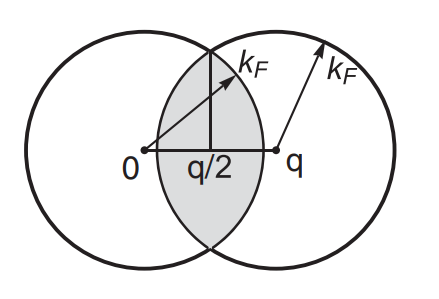
\includegraphics[scale=0.55]{figs/Jellium model/jellium_integration_region.png} }}
    \qquad
    \subfloat[\centering ]{{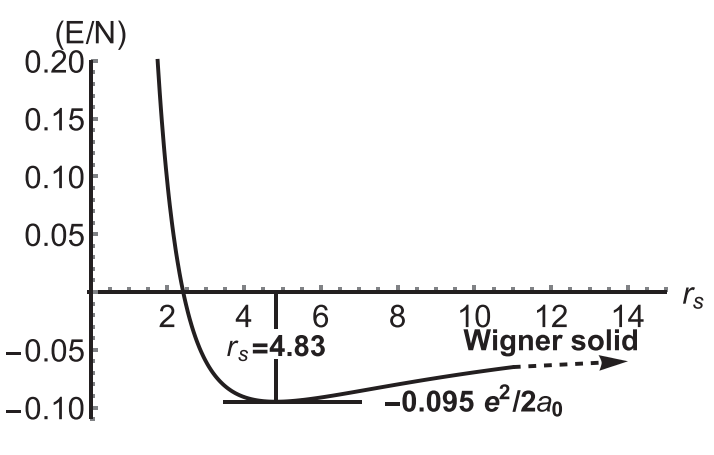
\includegraphics[scale=0.55]{figs/Jellium model/jellium_gse.png}}}
    \caption{Fig. A: Geometry for the ${\bf k}$-integration is shown for arbitrary, but fixed, ${\bf q}$, which is just the intersection of two spheres. \\
    Fig. B: Ground-state energy per electron, including first-order correction, for the jellium model.}
    \label{figs:jellium}
\end{figure}

\begin{equation}
    \begin{split}
        E^{(1)} &= \langle {\Omega} \bigg|  \sum_{\substack{{\bf k},{\bf k}',{\bf q} \in \Lambda\\
    \sigma \in \mathds{C}^2}} \frac{2\pi e^2}{\Omega q^2} {\bf c}_{{\bf k}+{\bf q} \blanky \sigma}^\dagger {\bf c}_{{\bf k}'-{\bf q} \blanky \sigma}^\dagger {\bf c}_{{\bf k}' \blanky \sigma} {\bf c}_{{\bf k} \blanky \sigma} \bigg| {\Omega} \rangle \\
    &= \langle {\Omega} \bigg|  \sum_{\substack{{\bf k},{\bf q} \in \Lambda\\
    \sigma \in \mathds{C}^2}} \frac{2\pi e^2}{\Omega q^2} {\bf c}_{{\bf k}+{\bf q} \blanky \sigma}^\dagger {\bf c}_{{\bf k} \sigma}^\dagger {\bf c}_{{\bf k}+{\bf q} \blanky \sigma} {\bf c}_{{\bf k} \sigma} \bigg| {\Omega} \rangle \\
    &= \langle {\Omega} \bigg|  \sum_{\substack{{\bf k},{\bf q} \in \Lambda\\
    \sigma \in \mathds{C}^2}} \frac{2\pi e^2}{\Omega q^2} (-N_{{\bf k}+{\bf q} \blanky \sigma} - N_{{\bf k} \sigma}) \bigg| {\Omega} \rangle  \Rightarrow \varepsilon^{(1)}({\bf k}) = - \frac{2\pi e^2}{\Omega} \sum_{{\bf q}} \frac{N_{{\bf k}} + {\bf q}}{q^2} \\
    \end{split}
\end{equation}
\begin{equation}
    \begin{split}
    \Rightarrow E^{(1)} &= -\frac{4\pi e^2}{\Omega} \frac{\Omega}{(2\pi)^6} \int_{\mathds{R}^6} d{\bf k} d{\bf q} \blanky \frac{1}{q^2} \Theta(k_F - |{\bf k} + {\bf q}|) \Theta(k_F - k) \textnormal{ with the integration region shown in \cref{figs:jellium} (left)}  \\
    &= - \frac{4\pi e^2 \Omega}{(2\pi)^6} \int_{\mathds{R}^3} \frac{d{\bf q}}{q^2} \int_{\mathds{R}^3} d{\bf p} \blanky \Theta\bigg(k_F - \bigg| {\bf p} + \frac{1}{2} {\bf q}\bigg|\bigg) \Theta\bigg(k_F - \frac{1}{2} {\bf q}\bigg) \\
    &= -\frac{e^2}{2a_0} N \frac{3}{2\pi} \bigg(\frac{9 \pi}{4}\bigg)^{\frac{1}{3}} \frac{1}{r_s}.
    \end{split}
\end{equation}

This results, shown in \cref{figs:jellium} (right), shows that the electron gas is stable when the repulsive Coulomb interaction is turned on. No external confinement potential is therefore needed to hold the electron gas in the ion jellium together. There exists an optimal density $n^*$, or interparticle distance $r_s^*$, which minimizes the energy and furthermore yields an $E^* < 0$. The negative exchange energy overcome the positive kinetic energy. This method of treating the electron gas is a special case of the Hartree-Fock approximation and is the simplest way to take into account interactions. The interesting point to note is that in this approximation the energy is reduced below that of the Sommerfeld gas, which is a manifestation of the exchange hole. 

\begin{figure}
    \centering
    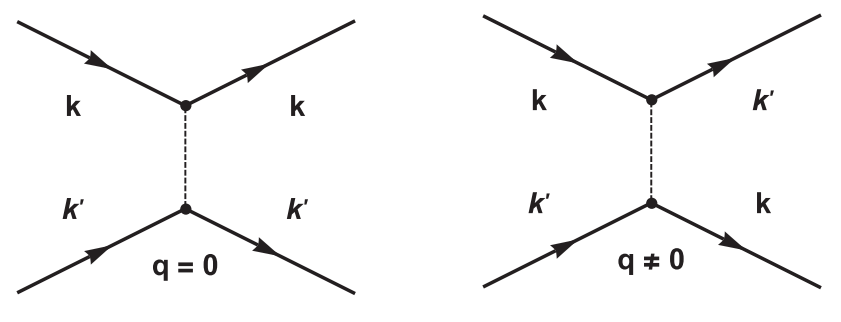
\includegraphics[scale  =.5]{figs/Jellium model/feynmann_diags.png}
    \caption{Diagrams for the jellium sea. The dashed line represents the interaction.}
    \label{fig:feynmann_jellium}
\end{figure}

\blanky \\

\paragraph{\textbf{Hartree-Fock approximation as a Mean-Field Theory}} \label{First_order_Hartree_Fock}\blanky \\

Consider the electronic Hamiltonian given by 
\cref{pre-HF-jellium H}. The goal is to write an effective two-body Hamiltonian, which takes into account the average effects of the interactions. Therefore, the four-Fermi interaction is replaced with a sum of all possible two-body terms

\begin{equation}
    \begin{split}
    \langle {\bf c}_1^\dagger {\bf c}_2^\dagger {\bf c}_3 {\bf c}_4 \rangle_{\textnormal{MFT}} &= - \langle {\bf c}_1^\dagger {\bf c}_3 \rangle {\bf c}_2^\dagger {\bf c}_4 -  \langle {\bf c}_2^\dagger {\bf c}_4 \rangle {\bf c}_1^\dagger {\bf c}_3 +  \langle {\bf c}_1^\dagger {\bf c}_4 \rangle {\bf c}_2^\dagger {\bf c}_3 +  \langle {\bf c}_2^\dagger {\bf c}_3 \rangle {\bf c}_1^\dagger {\bf c}_4, \\
    &\textnormal{ where } \langle {\bf c}_{{\bf k}\sigma}^\dagger {\bf c}_{{\bf k}'\sigma'} \rangle = {\bf n}_{{\bf k}\sigma} \delta_{{\bf k}{\bf k}'}^{\sigma \sigma'}
\end{split}\end{equation}

The mean field terms can be understood as the average number of particles ${\bf n}_{{\bf k}\sigma}$ in the $\ket{{{\bf k}\sigma}}$-state, which will be weighted with the two-body interaction $V({\bf q})$ to give the average interaction due to all other interaction terms. Then, the four-Fermi interaction in the mean-field approximation reads

\begin{equation}
\begin{split}
    \mathcal{V}_{\textnormal{HF}} = \frac{1}{2} \sum_{\substack{{\bf k}{\bf k}',{\bf q} \in \Lambda\\
    \sigma \sigma' \in \mathds{C}^2}} V({\bf q}) &\bigg[-\langle 
    {\bf c}_{{\bf k}\sigma}^\dagger {\bf c}_{{\bf k}'\sigma'}
    \rangle {\bf c}_{{\bf k}'-{\bf q} \blanky \sigma'}^\dagger {\bf c}_{{\bf k}-{\bf q} \sigma} 
    -  \langle {\bf c}_{{\bf k}'-{\bf q} \blanky \sigma'}^\dagger {\bf c}_{{\bf k}-{\bf q} \sigma}  \rangle {\bf c}_{{\bf k}\sigma}^\dagger {\bf c}_{{\bf k}'\sigma'} \\
    & \blanky \blanky \blanky + \langle {\bf c}_{{\bf k}\sigma}^\dagger {\bf c}_{{\bf k}-{\bf q} \sigma} \rangle {\bf c}_{{\bf k}'-{\bf q} \blanky \sigma'}^\dagger {\bf c}_{{\bf k}'\sigma'}
    +  \langle {\bf c}_{{\bf k}'-{\bf q} \blanky \sigma'}^\dagger {\bf c}_{{\bf k}'\sigma'} \rangle {\bf c}_{{\bf k}\sigma}^\dagger {\bf c}_{{\bf k}-{\bf q} \sigma} 
    \bigg] \\
    &= - \sum_{\substack{{\bf k}{\bf q} \in \Lambda\\
    \sigma \in \mathds{C}^2}} V({\bf q})  \langle {\bf c}_{{\bf k} \sigma}^\dagger {\bf c}_{{\bf k} \sigma} \rangle {\bf c}_{{\bf k}-{\bf q} \blanky \sigma}^\dagger {\bf c}_{{\bf k}-{\bf q} \blanky \sigma} + V(0) \sum_{\substack{{\bf k}{\bf k}' \in \Lambda\\
    \sigma \sigma' \in \mathds{C}^2}} \langle {\bf c}_{{\bf k} \sigma}^\dagger {\bf c}_{{\bf k} \sigma} \rangle  {\bf c}_{{\bf k}' \sigma'}^\dagger {\bf c}_{{\bf k}' \sigma'} \\
    &= \sum_{\substack{{\bf k} \in \Lambda\\
    \sigma \in \mathds{C}^2}} \bigg(-\sum_{{\bf q} \in \Lambda} {\bf n}_{{\bf k}+{\bf q} \sigma} V({\bf q}) + nV(0)\bigg){\bf c}_{{\bf k} \sigma}^\dagger {\bf c}_{{\bf k} \sigma}, \\
    \Rightarrow  {\bf H}^{\textnormal{HF}} &= \sum_{\substack{{\bf k} \in \Lambda\\
    \sigma \in \mathds{C}^2}} \varepsilon_{\bf k}^{\textnormal{HF}} {\bf c}_{{\bf k} \sigma}^\dagger {\bf c}_{{\bf k} \sigma}, \textnormal{ where } \begin{split}
        \varepsilon_{\bf k}^{\textnormal{HF}} &= \varepsilon_{\bf k} + \sum_{\substack{{\bf k}' \in \Lambda\\
    \sigma' \in \mathds{C}^2}} [V(0) - \delta_{\sigma\sigma'} V({\bf k}- {\bf k}')] {\bf n}_{{\bf k}' \sigma'} \\
        &= \varepsilon_{\bf k} + V(0) N - \sum_{\substack{{\bf k}' \in \Lambda\\
    \sigma' \in \mathds{C}^2}} V({\bf k}- {\bf k}') {\bf n}_{{\bf k'} \sigma'}.
    \end{split}
    \end{split}
\end{equation}

Note that the Hartree or direct Coulomb term, which represents the average interaction energy of the electron ${\bf k}\sigma$ with all the other electrons in the system, is a constant; when summed over all electron it cancels exactly with the constant arising from the sum of the self-energy of the positive background and the interaction energy of the electron gas with that of the background. The Fock, or exchange term, is a momentum-dependent shift. \\

\textbf{Problems with the Hartree-Fock Theory}

Although we argued that the Hartree-Fock approximation becomes a better approximation in the high-density limit for electron interacting via the Coulomb attraction, it never becomes exact. The Hartree-Fock energy correction is given by 

$$
    \varepsilon^{(1)}({\bf k}) = \frac{e^2 k_F}{4\pi^2} \bigg[\frac{k_F^2 - k^2}{kk_F} \log \bigg| \frac{k_F + k}{k_F - k}\bigg| + 2\bigg]
$$

The first term in parentheses has a logarithmic divergence in slope $k=kf$. This means that while the energy shift might be small compared to the Fermi energy, the Fermi velocity $v_F = \nabla_{{\bf k}} \varepsilon({\bf k})$, contains a non-finite term. This problem can be traced back to the long-range nature of the Coulomb force. Two electrons at large distances ${\bf x}-{\bf x}'$ do not feel the full $\frac{1}{|{\bf x}-{\bf x}'|}$-interaction, but a screened version due to the presence of the intervening medium, namely the electron gas, rearranges itself to cancel out the long-range part of $V$. \\

\underline{Electron Interaction in Second-order Perturbation Theory}

Trying to improve upon the first-order result by going to second-order perturbation theory yields a disastrous results for the matrix elements diverge. According to second-order perturbation theory, 

\begin{equation}
\frac{E^{(2)}}{N} = \frac{1}{N} \sum_{\substack{\ket{\psi} \in \mathds{H} \\
\ket{\psi} \neq \ket{\Omega}}} \frac{\bra{\Omega} {{\bf V}}_c \ket{\psi} \bra{\psi} {{\bf V}}_c \ket{\Omega}}{E^{(0)} - E_\psi}.
\end{equation}

\begin{figure}
    \centering
    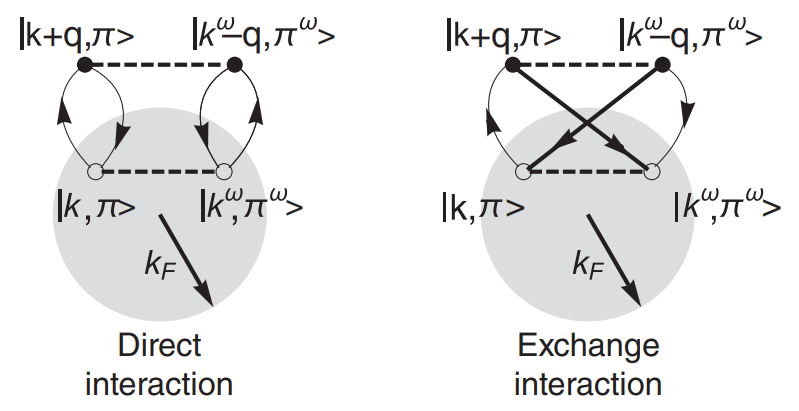
\includegraphics[scale = .5]{figs/Jellium model/fermi_sea_loops_second_order.png}
    \caption{The only two possible processes in second-order perturbation theory for two states, $\ket{{\bf k}_1, \sigma_1}$ and $\ket{{\bf k}_2, \sigma_2}$, in the Fermi sea. The direct process gives a divergent contribution to $\frac{E}{N}$ while the exchange process gives a finite contribution.}
    \label{fig:fermi_sea_loops_second_order}
\end{figure}

This, combined with the momentum-conserving Coulomb interaction, yields intermediate states where two particles are injected out of the Fermi sphere. From such an intermediate state, $\ket{\Omega}$, is restored by putting the excited electrons back into the holes they left behind. Therefore, the are only two types of possible processes: direct interaction and the exchange process, shown in \cref{fig:fermi_sea_loops_second_order}. \\

\begin{enumerate}
    \item In the \underline{Direct interaction}, it turns out that the direct interaction gives a divergent contribution $E^{(2)}_{\textnormal{dir}}$ to $E^{(2)}$ due to the singular behaviour of the Coulomb interaction at small ${\bf q}$-momentum transfers. The $(\ket{\psi} = \ket{\Omega})$-constraint leads to the second p
    
    $$
        \ket{\psi} = \Theta(|{\bf k}_1 + {\bf q}| - k_F) \Theta(|{\bf k}_2 - {\bf q}| - k_F) \Theta(k_F - |{\bf k}_2|) \Theta(k_F - |{\bf k}_1|) {\bf c}_{{\bf k}_1 + {\bf q}}^\dagger {\bf c}_{{\bf k}_2 - {\bf q}}^\dagger {\bf c}_{{\bf k}_2} {\bf c}_{{\bf k}_1} \ket{\Omega}.
    $$
    
    To restore $\ket{\Omega}$,  the same ${\bf q}$-momentum transfer must be involved in both $\bra{\Omega} {\bf V}_c \ket{\psi}$ and $\bra{\psi} {\bf V}_c \ket{\Omega}$, and writing ${\bf V}({\bf q}) = \frac{4 \pi e^2}{{\bf q}^2}$ yields
    
    \begin{equation}
    \begin{split}
    & E^{(2)}_{\textnormal{dir}} = \frac{1}{4 \Omega^2} \sum_{{\bf q} \in \Lambda} \sum_{\substack{{\bf k}{\bf k}' \in \Lambda\\
    \sigma \sigma' \in \mathds{C}^2}} \frac{{\bf V}({\bf q})^2}{E^{(0)} - E_{\nu}} \Theta(|{\bf k}_1 + {\bf q}| - k_F) \Theta(|{\bf k}_2 - {\bf q}| - k_F) \Theta(k_F - |{\bf k}_2|) \Theta(k_F - |{\bf k}_1|) \\
    & \textnormal{Given that ${\bf V}({\bf q})^2 \approx q^{-4}$} \Rightarrow E^{(0)} - E_{\psi} \overset{{\bf q} \rightarrow 0}{\approx} {\bf k}_1^2 + {\bf k}_2^2 - ({\bf k}_1+{\bf q})^2 - ({\bf k}_2 - {\bf q})^2 \approx q \\
    & \sum_{{\bf q} \in \Lambda} \sum_{\substack{{\bf k}{\bf k}' \in \Lambda\\
    \sigma \sigma' \in \mathds{C}^2}} \cdots \Theta(|{\bf k}_2 - {\bf q}| - k_F) \Theta(k_F - |{\bf k}_2|) \Theta(k_F - |{\bf k}_1|)  \overset{{\bf q} \rightarrow 0}{\approx} q \\
    & \Rightarrow E^{(2)}_{\textnormal{dir}} = \int_{0} dq q^2 \frac{1}{q^4} \frac{1}{q} q q = \int_{0} \frac{dq}{q} = \log q|_{0} \rightarrow \infty.
    \end{split}
    \end{equation}
    
    \blanky \\
    
    \item The exchange process does not lead to a divergence since, in this case, the momentum transfer in the excitation part is ${\bf q}$, but in the relaxation part it is ${\bf k}_2-{\bf k}_1-{\bf q}$. Thus ${\bf V}^2({\bf q})$ is replaced by ${\bf V}^2({\bf q}){\bf V}({\bf k}_2-{\bf k}_1-{\bf q}) \propto q^{-2}$ for ${\bf q} \rightarrow 0$, which is less singular than ${\bf V}^2({\bf q}) \propto q^{-4}$. \\  
\end{enumerate}

Physically, the energy of an electron gas must be finite. The only hope for rescue lies in regularization of the divergent behaviour by taking higher-order perturbation terms into account. Consider now the ground-state energy of the jellium model of a three-dimensional electron gas. In the $(r_s < 1)$-regime, this energy can be expressed in terms of a power-series in $r_s$, as

$$
    E_0 = \frac{K}{r_s^2} [1+ br_s + c r_s^2 + \cdots],
$$

where $K, a,b,c$ are constants. This is not exactly right, since first-order perturbation theory gives a term of the $(br_s)$-form in the series. But, considering second-order perturbation theory, one finds a contribution that diverges like $\int_0 \frac{dq}{q}$, where $q$ is the transfer-momentum in the Fourier transform ${\bf V}_q$ of the Coulomb interaction, ${\bf V}_q \approx q^{-2}$. Thus, there is in fact a logarithmic divergence from the lower limit $0$ of the momentum transfers. This divergence is associated with the long range of the Coulomb interaction. Furthermore, if one examines higher-order terms in the perturbation series, one finds that they diverge even more strongly. \\

On physical grounds, however, the energy of the interacting electron gas must be finite and well-defined, with no phase transitions occurring as the repulsive interactions are turned on. This failure of standard perturbation theory appears to signal that the energy does not have a standard power-series expansion in $r_s$. In 1957, Gell-Mann and Bruckner resolved this issue by developing many-body perturbation theory\footnote{Many-body perturbation expansions without diagrams.
I. Normal states. Behnam Farid §}, in which the summation of the divergent terms in the series an infinite number of terms) is performed before doing the momentum integrals, thus arriving to a finite and well-defined results. This is called the resummation of the perturbation series. They found that there was a term in the series for $E_0$ that is $\propto \log r_s$, and is non-analytic at $r_s = 0$. This holds so long the interaction doesn't cause any drastic changes to the system, such as a phase transition. \\

\subsection{Random Phase Approximation}

In the second quantization formalism, the fermionic field operators may be written in plane-wave basis as 

$$
    \Psi({\bf x}, t) = \frac{1}{\sqrt{\Omega}} \sum_{{\bf k} \in \Lambda} e^{i {\bf k} \cdot {\x}} {\bf c}_{{\bf k}}, \blanky \blanky \blanky \blanky 
    \Psi^\dagger({\bf x}, t) = \frac{1}{\sqrt{\Omega}} \sum_{{\bf k} \in \Lambda} e^{-i {\bf k} \cdot {\x}} {\bf c}_{{\bf k}}^\dagger.
$$

The particle density $\rho({\bf x})$ at point ${\bf x}$ is given by 

$$
    \rho({\bf x}) = \sum_{i \in \mathds{N}} \delta({\bf x} - {\bf x}_i) \Rightarrow \rho({\bf x}) = \int_{\mathds{R}^3} d{\bf x} \blanky \Psi^\dagger({\bf x}) \bigg(\sum_{i \in \mathds{N}} \delta({\bf x} - {\bf x}_i)\bigg) \Psi({\bf x}) = \sum_{i \in \mathds{N} }\Psi^\dagger({\bf x}) \Psi({\bf x}). 
$$

Its Fourier transform is given by ${\rho_{{\bf q}}} = \sum_{{\bf k} \in \Lambda} {\bf c}_{{\bf k}+{\bf q}}^\dagger {\bf c}_{\bf k}$. Its physical meaning is straightforward: it gives rise to particle-hole pairs charge fluctuations around the Fermi surface. Since $\rho^\dagger = \rho$, it follows that $\rho_{{\bf q}}^\dagger = \rho_{-{\bf q}}$. \footnote{For example, the following four-body term may be recast as 

$$
\sum_{{\bf k, k'} \in \Lambda} {\bf c}_{{\bf k}-{\bf q}}^\dagger {\bf c}_{{\bf k}'+{\bf q}}^\dagger {\bf c}_{{\bf k}'} {\bf c}_{{\bf k}} = - \sum_{{\bf k'} \in \Lambda} {\bf n}_{{\bf k}'} + \rho_{{\bf q}} \rho_{-{\bf q}'}.
$$}\\

Now, the following question naturally arises. Under what conditions an interacting system, with Hamiltonian 

$$
    {\bf H} = \sum_{{\bf k} \in \Lambda} \varepsilon_{{\bf k}} {\bf c}_{{\bf k}}^\dagger {\bf c}_{{\bf k}} + \frac{1}{2} \sum_{{\bf q} \in \Lambda} {\bf V}_{{\bf q}} (\rho_{{\bf q}} \rho_{-{\bf q}} - N),
$$

and ground-state $\ket{\Omega}$, ${\bf H} \ket{\Omega} = \varepsilon_0 \ket{\Omega}$, can support density excitations associated with $\rho_{{\bf q}}$? Namely, these excitations are

$$
    {\bf H} \rho_{{\bf q}}^\dagger \ket{\Omega} = (\varepsilon_0 + \hbar \omega_{{\bf q}}) \rho_{{\bf q}}^\dagger \ket{\Omega}
$$

\blanky \\

The previous equation may be rewritten as 

\begin{equation} 
\begin{split}
    [{\bf H}, \rho_{\bf q}^\dagger] = \hbar \omega_{{\bf q}} \rho_{{\bf q}}^\dagger  \Rightarrow & \bigg[\sum_{{\bf k} \in \Lambda} \varepsilon_{{\bf k}} {\bf c}_{{\bf k}}^\dagger {\bf c}_{{\bf k}} + \frac{1}{2} \sum_{{\bf q} \in \Lambda} {\bf V}_{{\bf q}} (\rho_{{\bf q}} \rho_{-{\bf q}} - N), \rho_{\bf q}^\dagger \bigg] = \hbar \omega_{{\bf q}} \rho_{{\bf q}}^\dagger \\
    & \bigg[\sum_{{\bf k} \in \Lambda} \varepsilon_{{\bf k}} {\bf c}_{{\bf k}}^\dagger {\bf c}_{{\bf k}}, \rho_{\bf q}^\dagger\bigg] + \frac{1}{2} \bigg[\sum_{{\bf q} \in \Lambda} {\bf V}_{{\bf q}} (\rho_{{\bf q}} \rho_{-{\bf q}} - N), \rho_{\bf q}^\dagger \bigg] = \\
    & \sum_{{\bf k} \in \Lambda} \varepsilon_{{\bf k}} \bigg[ {\bf c}_{{\bf k}}^\dagger {\bf c}_{{\bf k}}, \rho_{\bf q}^\dagger\bigg] + \frac{1}{2} \sum_{{\bf q} \in \Lambda} {\bf V}_{{\bf q}} \cancel{\bigg[\rho_{{\bf q}} \rho_{-{\bf q}}, \rho_{\bf q}^\dagger\bigg]} = \\
    & \sum_{{\bf k}, \mathfrak{k} \in \Lambda} \varepsilon_{{\bf k}} \bigg[ {\bf c}_{{\bf k}}^\dagger {\bf c}_{{\bf k}}, {\bf c}_{{\bf q}} {\bf c}_{{\bf \mathfrak{k} + q}}^\dagger \bigg] =  \\
    &\sum_{{\bf k}, \mathfrak{k} \in \Lambda} \varepsilon_{{\bf k}} \bigg({\bf c}_{{\bf k}}^\dagger \cancel{[{\bf c}_{{\bf k}}, {\bf c}_{{\bf q}}]} {\bf c}_{{\bf \mathfrak{k} + q}}^\dagger + [{\bf c}_{{\bf k}}^\dagger, {\bf c}_{{\bf q}}] {\bf c}_{{\bf k}} {\bf c}_{{\bf k}}^\dagger + {\bf c}_{{\bf q}} {\bf c}_{{\bf k}}^\dagger [{\bf c}_{{\bf k}}, {\bf c}_{{\bf \mathfrak{k} + q}}^\dagger] + {\bf c}_{{\bf q}} \cancel{[{\bf c}_{{\bf k}}^\dagger, {\bf c}_{{\bf \mathfrak{k} + q}}^\dagger]} {\bf c}_{{\bf k}} \bigg) = \\
    & \sum_{{\bf k} \in \Lambda} (\varepsilon_{{\bf k + q}} - \varepsilon_{{\bf k}}) {\bf c}_{{\bf {\bf k} + q}}^\dagger {\bf c}_{{\bf k}} = 
\end{split}
\end{equation}

If $\rho_{{\bf q}}^\dagger$ actually creates an excitation of energy $\hbar \omega$, then 

\begin{equation}
\begin{split}
    [{\bf H}, [{\bf H}, \rho_{\bf q}^\dagger]] = (\hbar \omega)^2 \rho_{{\bf q}}^\dagger \\
    \Rightarrow (\hbar \omega)^2 \rho_{{\bf q}}^\dagger &= \sum_{{\bf k} \in \Lambda} (\varepsilon_{{\bf k + q}} - \varepsilon_{{\bf k}}) [{\bf H}, {\bf c}_{{\bf {\bf k} + q}}^\dagger {\bf c}_{{\bf k}}] = \sum_{{\bf k} \in \Lambda} (\varepsilon_{{\bf k + q}} - \varepsilon_{{\bf k}})^2 {\bf c}_{{\bf k + q}}^\dagger {\bf c}_{{\bf k}} \\
    & \blanky \blanky \blanky \blanky+ \sum_{{\bf k}, {\bf q}' \in \Lambda} (\varepsilon_{{\bf k + q}} - \varepsilon_{{\bf k}}) \frac{V_{{\bf q}'}}{2} \bigg[({\bf c}_{{\bf {\bf k} + q - q'}}^\dagger {\bf c}_{{\bf k}} - {\bf c}_{{\bf k + q}}^\dagger {\bf c}_{{\bf {\bf k} + q'}}) \rho_{{\bf q}'}^\dagger + \rho_{{\bf q}'} ({\bf c}_{{\bf {\bf k} + q + q'}}^\dagger {\bf c}_{{\bf k}} - {\bf c}_{{\bf k + q}}^\dagger {\bf c}_{{\bf {\bf k} - q'}})\bigg] \\
    &= \sum_{{\bf k} \in \Lambda} \bigg[ \frac{\hbar^2}{2m} (2 {\bf k} \cdot {\bf q} + {\bf q}^2)\bigg]^2 {\bf c}_{{\bf k}+{\bf q}}^\dagger {\bf c}_{{\bf k}} + \sum_{{\bf k}, {\bf q}' \in \Lambda} \frac{V_{\bf q'}}{2}\bigg[\frac{\hbar^2}{2m}(2 {\bf k}\cdot {\bf q} + {\bf q}^2) ({\bf c}_{{\bf {\bf k} + q - q'}}^\dagger {\bf c}_{{\bf k}} - {\bf c}_{{\bf k + q}}^\dagger {\bf c}_{{\bf {\bf k} + q'}}) \\ & \blanky \blanky \blanky \blanky - \frac{\hbar^2}{2m}(2 {\bf k}\cdot {\bf q} + {\bf q}^2) ({\bf c}_{{\bf {\bf k} + q + q'}}^\dagger {\bf c}_{{\bf k}} - {\bf c}_{{\bf k + q}}^\dagger {\bf c}_{{\bf {\bf k} - q'}})\bigg] \\
    &= \sum_{{\bf k} \in \Lambda} \bigg[ \frac{\hbar^2}{2m} (2 {\bf k} \cdot {\bf q} + {\bf q}^2)\bigg]^2 {\bf c}_{{\bf k}+{\bf q}}^\dagger {\bf c}_{{\bf k}} + \sum_{{\bf q}' \in \Lambda} \frac{V_{\bf q'}}{2} \bigg[ \sum_{{\bf k} \in \Lambda}\frac{\hbar^2}{2m}(2 {\bf k}\cdot {\bf q} + {\bf q}^2) ({\bf c}_{{\bf {\bf k} + q - q'}}^\dagger {\bf c}_{{\bf k}} - {\bf c}_{{\bf k + q}}^\dagger {\bf c}_{{\bf {\bf k} + q'}}) \\ 
    & \blanky \blanky \blanky \blanky - \sum_{{\bf k} \in \Lambda}\frac{\hbar^2}{2m}(2 {\bf k}\cdot {\bf q} + {\bf q}^2) ({\bf c}_{{\bf {\bf k} + q + q'}}^\dagger {\bf c}_{{\bf k}} - {\bf c}_{{\bf k + q}}^\dagger {\bf c}_{{\bf {\bf k} -
    q'}})\bigg] \\
    &= \sum_{{\bf k} \in \Lambda} \bigg[ \frac{\hbar^2}{2m} (2 {\bf k} \cdot {\bf q} + {\bf q}^2)\bigg]^2 {\bf c}_{{\bf k}+{\bf q}}^\dagger {\bf c}_{{\bf k}} \\
    & + \sum_{{\bf q}' \in \Lambda} \frac{V_{\bf q'}}{2} \bigg[ \sum_{{\bf k} \in \Lambda}\frac{\hbar^2}{2m}(2 {\bf k}\cdot {\bf q} + {\bf q}^2) {\bf c}_{{\bf {\bf k} + q - q'}}^\dagger {\bf c}_{{\bf k}} - \frac{\hbar^2}{2m}(2 {\bf k}\cdot {\bf q} + {\bf q}^2) {\bf c}_{{\bf k + q}}^\dagger {\bf c}_{{\bf {\bf k} + q'}} \\
    & \blanky \blanky \blanky \blanky - \sum_{{\bf k} \in \Lambda}\frac{\hbar^2}{2m}(2 {\bf k}\cdot {\bf q} + {\bf q}^2) {\bf c}_{{\bf {\bf k} + q + q'}}^\dagger {\bf c}_{{\bf k}} - \frac{\hbar^2}{2m}(2 {\bf k}\cdot {\bf q} + {\bf q}^2) {\bf c}_{{\bf k + q}}^\dagger {\bf c}_{{\bf {\bf k} - q'}}\bigg] \\
    \end{split}
\end{equation}

\begin{equation}
    \begin{split}
 \blanky  
&= \sum_{{\bf k} \in \Lambda} \bigg[ \frac{\hbar^2}{2m} (2 {\bf k} \cdot {\bf q} + {\bf q}^2)\bigg]^2 {\bf c}_{{\bf k}+{\bf q}}^\dagger {\bf c}_{{\bf k}} \blanky \blanky \blanky \blanky \blanky \blanky \textnormal{  let ${\bf k}' = {\bf k} + {\bf q}'$, ${\bf k}'' = {\bf k} - {\bf q}'$}\\
 & \blanky \blanky \blanky \blanky + \sum_{{\bf q}' \in \Lambda} \frac{V_{\bf q'}}{2} \bigg[ \sum_{{\bf k} \in \Lambda}\frac{\hbar^2}{2m}(2 {\bf k}\cdot {\bf q} + {\bf q}^2) {\bf c}_{{\bf {\bf k} + q - q'}}^\dagger {\bf c}_{{\bf k}} - \sum_{{\bf k}' \in \Lambda}\frac{\hbar^2}{2m}(2 ({\bf k}' - {\bf q}')\cdot {\bf q} + {\bf q}^2) {\bf c}_{{\bf k' + q - q'}}^\dagger {\bf c}_{{\bf {\bf k}'}}\\ 
 & \blanky \blanky \blanky \blanky - \sum_{{\bf k} \in \Lambda}\frac{\hbar^2}{2m}(2 {\bf k}\cdot {\bf q} + {\bf q}^2) {\bf c}_{{\bf {\bf k} + q + q'}}^\dagger {\bf c}_{{\bf k}} - \sum_{{\bf k}'' \in \Lambda}\frac{\hbar^2}{2m}(2 ({\bf k}'' + {\bf q}')\cdot {\bf q} + {\bf q}^2) {\bf c}_{{\bf k'' + q + q'}}^\dagger {\bf c}_{{\bf {\bf k}''}} \bigg] \\
    \end{split}
\end{equation}

\begin{align}
     \alignedbox{(\hbar \omega)^2 \rho_{{\bf q}}^\dagger}{= \sum_{{\bf k} \in \Lambda} \bigg[ \frac{\hbar^2}{2m} (2 {\bf k} \cdot {\bf q} + {\bf q}^2)\bigg]^2 {\bf c}_{{\bf k}+{\bf q}}^\dagger {\bf c}_{{\bf k}} + \sum_{{\bf q}' \in \Lambda} \frac{V_{\bf q'}}{2} \frac{\hbar^2 {\bf q} \cdot {\bf q}'}{m} \bigg(\rho_{{\bf q}' - {\bf q}} \rho_{{\bf q}'}^\dagger - \rho_{{-{\bf q}'}}^\dagger \rho_{-{\bf q} - {\bf q}'} \bigg).}
     \label{RPA-basis equation}
\end{align}

\begin{figure}
    \centering
    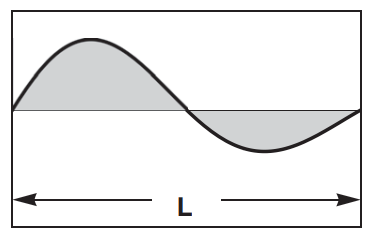
\includegraphics[scale = .5]{figs/Jellium model/RPA-fig.png} 
    \caption{Consider a length-$L$ box. Then, $\rho_q$ measures the quantity approximately equal to the difference in the particle number in the two halves of the container. }
    \label{fig:RPA-box}
\end{figure}

Now, in order to study \cref{RPA-basis equation}, note that $\rho_0$ is actually much larger than all the other components. It is just the average particle density in the system. Consider a box of length-$L$, shown in \cref{fig:RPA-box}, containing a large number of electrons of $\rho_0$ average density, then $\rho_0$'s first Fourier component is 

$$
    \int_{\Omega \subset \R^3} d{\bf x} \blanky \rho({\bf x}) e^{\frac{2i \pi x}{L}},
$$

will be approximately equal to the difference between the particle number in the left and right hand sides of the box, the gray area. The number difference will then be small, compared to the total number and so $\rho_0$ will prevail in the summation over ${\bf q}'$. Since the $({\bf q}' = 0)$-term is omitted, $\rho_0$ will only appear when ${\bf q}' = \pm {\bf q}$. The neglect of all other terms, when ${\bf q}' \neq \pm {\bf q}$ is known as the \textbf{random phase approximation} \footnote{An alternative interpretation for the RPA is as follows. Consider the first-quantized version of the density operator $\rho_{{\bf q} \in \Lambda} = \frac{1}{\Omega} \sum_{n \in \mathds{N}} e^{i {\bf q} \cdot {\bf x}_n}$, where ${\bf x}_n$ is the $n$-th's particles position. Then, $\rho_{{\bf q} \pm {\bf q}'}$ may be written in first quantized form as 

$$
    \rho_{{\bf q} \pm {\bf q}'} \frac{1}{\Omega} \sum_{n \in \mathds{N}} e^{i ({\bf q} \pm {\bf q}') \cdot {\bf x}_n}.
$$

Then, if the electrons are statistically randomly distributed in the system, the preceding sum only gives a finite result if ${\bf q} = \mp {\bf q'}$, since the sum involves random phases that add destructively. In RPA, \cref{RPA-basis equation} is approximated by keeping only terms with ${\bf q} = \mp {\bf q}'$. }.\\

\underline{Plasma oscillations}

Consider the case where ${\bf q}$ is small enough that, for the moment, the first term in \cref{RPA-basis equation} may be neglected and the second term approximated via RPA. In that case, 

$$
(\hbar \omega)^2 \rho_{{\bf q}}^\dagger = \frac{4\pi e^2}{q^2} \frac{\hbar^2 q^2}{m} (\rho_0 \rho_{{\bf q}}^\dagger + \rho_{{\bf q}}^\dagger \rho_0 ) \rightarrow \omega^2 = \frac{4\pi e^2 \rho_0}{m},
$$

which gives just the classical plasma frequency $\omega_P$. The contribution of the first term may be approximated by setting $k \sim k_F$ and $\langle 2 {\bf k}_F \cdot {\bf q} \rangle >> {\bf q}^2$. Averaging over all angles yields

$$
\langre ({\bf k}_F \cdot {\bf q})^2 \rangle \simeq \frac{1}{4\pi} 4\pi^2 k_F^2 q^2 \int_{-1}^{1} dx x^2 = 2\pi k_F^2 q^2, 
$$

which yield the plasmon dispersion relation

$$
\omega^2({\bf q}) = \omega_P^2 + \frac{2\pi \hbar^2 k_F^2}{3m^2} q^2 \simeq \omega_P + \frac{\pi v_F^2}{3\omega_P} q^2. 
$$

Thus, the relevant long-wavelength excitations are collective motions of the electron gas. Bohm and Pines suggested that electrons act as interacting particles through a bare Coulomb potential $\frac{4\pi e^2}{q^2}$ only for length scales less than an effective screening length, which may be taken to be the Thomas-Fermi distance, $\sim q_{\textnormal{TF}}^{-1}$. Below $q_{\textnormal{TF}}$, the interaction contribute only to the plasma oscillations. \\

\subsection{Green Functions for Many-Body systems.}

Green function techniques play a fundamental role in the treatment of many-body systems, for many properties of a many body system -eg. ground state energy, excitation spectra, response functions, electric and magnetic susceptibilities and thermodynamic quantities- can be derived from many-body Green functions.\\

Consider the ground state $\ket{\Omega}$ of a system. At some time $t'$, a perturbation is enacted upon the system, said perturbation represented by a local operator ${\bf O}^\dagger({\bf x}, t)$, creating an initial state ${\bf O}^\dagger({\bf x}', t') \ket{\Omega}$. Thus, the system has been deviated from the initial some by some local excitations, a disturbance, and then this disturbance will evolve in space and time. Such a scenario describes typical local measurements done on a quantum many-particle system. Since an explicit time dependence is necessary for this formalism, the Heisenberg picture is useful. To determine physically interesting quantities, the quantum-mechanical amplitude to find the system in state ${\bf O}^\dagger({\bf x}', t') \ket{\Omega}$ at time $t > t'$ namely, 

$$
    \mathcal{A} = \bra{\Omega} {{\bf O}}({{\bf x}}, t) {{\bf O}}^\dagger({{\bf x}}', t') \ket{\Omega}.
$$

Many quantum-mechanical operators may be written in bilinear forms of the field operators themselves, $\hat{\Psi}({{\bf x}}, t)$. However, it turns out that correlation functions of the field operators are related to experiments such as photoemission and tunnelling spectroscopies, which involve extraction or injection of a single electron. These field correlation functions can be identified as propagators which satisfy the Green function equation. \\

\subsubsection{The One-Particle Green Function of Many-Body Systems}

\paragraph{Non-interacting Particle Propagator}

Consider a particle in free space described by a single-particle time-independent Hamiltonian ${\bf H}_1$. Its eigenstates and eigenenergies are 

$$
    {\bf H}_1 \ket{\phi_n} = \varepsilon_n \ket{\phi_n}.
$$

In general, if a particle is in the $\ket{\phi}_i$-state, it will remain in that state forever. Instead, consider a system in a generic state $\ket{\psi_{\textnormal{trial}}}$. If the trial state is created at time $t'$, the wave-function at a later time $t$ is given by 

$$
    \ket{\psi(t)} = e^{-\frac{i {\bf H} (t-t')}{\hbar}} \ket{\psi_{\textnormal{trial}}} = \sum_{n} \ket{\psi_n} e^{-\frac{i \varepsilon_n (t-t')}{\hbar}} \bar{\phi_n}\ket{\psi_{\textnormal{trial}}}.
$$

Then, at time $t$, the probability amplitude that a measurement would find the particle at position ${\bf x}$ can be found as

\begin{equation}
    \begin{split}
        \bra{{\bf x}} \ket{\psi(t)} \Theta(t-t') &= \int_{\R^3} d{\bf x}' \blanky \bra{{\bf x}} e^{-\frac{i {\bf H} (t-t')}{\hbar}} \ket{{\bf x}'}\bra{{\bf x}'} \ket{\psi_{\textnormal{trial}}} \Theta(t-t') \\
        &=  \int_{\R^3} d{\bf x}' \sum_{n \in \mathds{N}} \blanky \bra{{\bf x}} \ket{\phi_n} e^{-\frac{i \varepsilon_n (t-t')}{\hbar}} \bra{\phi_n}\ket{{\bf x}'}\bra{{\bf x}'} \ket{\psi_{\textnormal{trial}}} \Theta(t-t') \\
        &= i \int_{\R^3} d{\bf x}' \blanky \mathfrak{G}^{\textnormal{R}}({\bf x}t, {\bf x}'t') \psi_{\textnormal{trial}}({\bf x}', t'), \begin{array}{c}
             \textnormal{ where } \mathfrak{G}^{\textnormal{R}}({\bf x}t, {\bf x}'t') = - i \Theta(t-t') \bra{{\bf x}} e^{-\frac{i {\bf H} (t-t')}{\hbar}} \ket{{\bf x}'} \\
             \textnormal{ is the retarded Green function, or propagator,} \\
             \textnormal{ in coordinate representation.}
        \end{array}
    \end{split} 
    \label{NR-1particle-GF}
\end{equation}

Note that the time translational invariance is apparent due to the Hamiltonian's dependence on $\tau = t-t'$. Therefore, if the Green function $\mathfrak{G}^{\textnormal{R}}({\bf x}t, {\bf x}'t')$ is known, then it can be used to calculate the evolution of any initial state. Interesting information can be extracted from the propagator. 

\begin{itemize}
    \item The bracket $\bra{\phi_n}\ket{{\bf x}} = \bra{\phi_n} \psi_n^\dagger({\bf x}) \ket{0}$ is just the probability amplitude of forcing the system to collapse into the eigenstate $\ket{\psi_n}$ when a particle is inserted at position ${\bf x}$ and its energy is measured immediately afterwards. \\
    \item Its resolvant can also be found. From \cref{NR-1particle-GF}, note that the time evolution is a superposition of waves propagating with different energies. In principle, it could be used to determine the eigenspectrum. This can be done via a Fourier transform to the frequency domain\footnote{Note that the Fourier transform is ill-defined, given the oscillatory behaviour for $t \rightarrow \infty$. Therefore, according to the Sokhotoski-Plemelj formula, the new function
        $$
            e^{-\eta |t| }\mathfrak{G}^{\textnormal{R}}({\bf x}, {\bf x}'; \omega), \textnormal{ with } \eta > 0,
        $$
        is considered.},
    
    \begin{equation}
    \begin{split}
        \mathfrak{G}^{\textnormal{R}}({\bf x}, {\bf x}'; \omega) &= \mathcal{F}[        \mathfrak{G}^{\textnormal{R}}({\bf x}t, {\bf x}'t')]({\bf x}, {\bf x}'; \omega) \\
        &= \int dt \blanky e^{i(\omega + i \eta) \tau} \bra{{\bf x}} e^{-\frac{i {\bf H} \tau}{\hbar}} \ket{{\bf x}'} = \bigg\langle {\bf x} \bigg| \frac{1}{\omega - {\bf H} + i \eta} \bigg| {{\bf x}'}\bigg\rangle,
    \end{split}
    \end{equation}
    
    where the Sokhotoski-Plemelj formula has been used. This is just the resolvent whose poles constitute the quantum system's spectrum. \\
    
    Operationally, we can dvise a gedankenexperiment in which the particle is initially inserted at ${\bf x}'$-position and picked up at ${\bf x}$-position after some time $t$. When performing this recipe with adequate resolution and for a sufficiently large number of different positions and elapsed times, the Fourier transform of the record data would provide the full eigenvalue spectrum. Such an experiment would give complete information on our particle. 
\end{itemize}

This scenario thus reveals that all observables can be expressed in terms of the Green function and thus avoid the explicit use of the wavefunctions. \\

\underline{Differential Equation for the Green Function} \\

Consider \cref{NR-1particle-GF}. The LHS's time derivative will yield

\begin{equation}
    \begin{split}
        &\bra{{\bf x}} \ket{\psi(t)} \Theta(t-t') = i \int_{\R^3} d{\bf x}' \blanky \mathfrak{G}^{\textnormal{R}}({\bf x}t, {\bf x}'t') \psi_{\textnormal{trial}}({\bf x}', t') \\
        &i \delta(t-t') \psi({\bf x}, t) + i \Theta(t-t') \frac{\partial \psi({\bf x}, t)}{\partial t} = i \frac{\partial}{\partial t} \bigg(i \int_{\R^3} d{\bf x}' \blanky \mathfrak{G}^{\textnormal{R}}({\bf x}t, {\bf x}'t') \psi({\bf x}', t') \bigg) \\
        & i \delta(t-t') \int_{\R^3} d{\bf x}' \blanky \delta({\bf x}- {\bf x}') \psi({\bf x}, t) + {\bf H} \Theta(t-t') ({\bf x}) \frac{\partial \psi({\bf x}, t)}{\partial t} = i \frac{\partial}{\partial t} \bigg(i \int_{\R^3} d{\bf x}' \blanky \mathfrak{G}^{\textnormal{R}}({\bf x}t, {\bf x}'t') \psi({\bf x}', t') \bigg) \\
        & i \delta(t-t') \int_{\R^3} d{\bf x}' \blanky \delta({\bf x}- {\bf x}') \psi({\bf x}, t) + {\bf H} \bigg(i \int_{\R^3} d{\bf x}' \blanky \mathfrak{G}^{\textnormal{R}}({\bf x}t, {\bf x}'t') \psi_{\textnormal{trial}}({\bf x}', t')\bigg) = i \frac{\partial}{\partial t} \bigg(i \int_{\R^3} d{\bf x}' \blanky \mathfrak{G}^{\textnormal{R}}({\bf x}t, {\bf x}'t') \psi({\bf x}', t') \bigg) \\
        &\int_{\R^3} d{\bf x}' \blanky \bigg(i \frac{\partial}{\partial t} - {\bf H}\bigg) \mathfrak{G}^{\textnormal{R}}({\bf x}t, {\bf x}'t') \psi({\bf x}', t') = i \delta(t-t') \int_{\R^3} d{\bf x}' \blanky \delta({\bf x}- {\bf x}') \psi({\bf x}, t) \\
        & \Rightarrow  \bigg(i \frac{\partial}{\partial t} - {\bf H}\bigg) \mathfrak{G}^{\textnormal{R}}({\bf x}t, {\bf x}'t') = \delta(t-t') \delta({\bf x}- {\bf x}'),
    \end{split}
\end{equation}

which is just the definition of the Green function for the Schr\"odinger equation in differential equation form
\iffalse\footnote{Another, equivalent deriviation is as follows,

\begin{equation}
    \begin{split}
        &\bra{{\bf x}} \ket{\psi(t)} \Theta(t-t') = i \int_{\R^3} d{\bf x}' \blanky \mathfrak{G}^{\textnormal{R}}({\bf x}t, {\bf x}'t') \psi_{\textnormal{trial}}({\bf x}', t') \\
        &i \delta(t-t') \psi({\bf x}, t) + i \Theta(t-t') \frac{\partial \psi({\bf x}, t)}{\partial t} = i \frac{\partial}{\partial t} \bigg(i \int_{\R^3} d{\bf x}' \blanky \mathfrak{G}^{\textnormal{R}}({\bf x}t, {\bf x}'t') \psi({\bf x}', t') \bigg) \\
        & i \delta(t-t') \psi({\bf x}, t) + \Theta(t-t') {\bf H}({\bf x}) \frac{\partial \psi({\bf x}, t)}{\partial t} = i \int_{\R^3} d{\bf x}' \blanky \frac{\partial}{\partial t} \bigg( - i \Theta(t-t') \bra{{\bf x}} e^{-\frac{i {\bf H} (t-t')}{\hbar}} \ket{{\bf x}'}\bigg) \psi({\bf x}', t') \\
        &  i \delta(t-t') \psi({\bf x}, t) + \Theta(t-t') {\bf H}({\bf x}) \frac{\partial \psi({\bf x}, t)}{\partial t} = i \int_{\R^3} d{\bf x}' \blanky \bigg(\frac{\partial}{\partial t} \Theta(t-t')\bigg) \bra{{\bf x}} e^{-\frac{i {\bf H} (t-t')}{\hbar}} \ket{{\bf x}'} \psi({\bf x}', t') \\
        & \blanky\blanky\blanky\blanky\blanky\blanky\blanky\blanky\blanky\blanky\blanky\blanky\blanky\blanky\blanky\blanky\blanky\blanky\blanky\blanky\blanky\blanky\blanky\blanky\blanky\blanky\blanky\blanky\blanky\blanky\blanky\blanky \blanky\blanky\blanky\blanky\blanky\blanky\blanky\blanky\blanky\blanky\blanky\blanky\blanky\blanky\blanky\blanky\blanky\blanky\blanky\blanky\blanky\blanky\blanky\blanky\blanky\blanky\blanky\blanky\blanky\blanky\blanky\blanky\blanky\blanky\blanky\blanky\blanky\blanky\blanky\blanky\blanky\blanky\blanky\blanky\blanky + i \int_{\R^3} d{\bf x}' \blanky \Theta(t-t') \bigg(\frac{\partial}{\partial t} \bra{{\bf x}} e^{-\frac{i {\bf H} (t-t')}{\hbar}} \ket{{\bf x}'} \bigg) \psi({\bf x}', t')\\
        &  i \delta(t-t') \psi({\bf x}, t) + \Theta(t-t') {\bf H}({\bf x}) \frac{\partial \psi({\bf x}, t)}{\partial t} = i \int_{\R^3} d{\bf x}' \blanky \delta(t-t') \bra{{\bf x}} e^{-\frac{i {\bf H} (t-t')}{\hbar}} \ket{{\bf x}'} \psi({\bf x}', t') \\
        & \blanky\blanky\blanky\blanky\blanky\blanky\blanky\blanky\blanky\blanky\blanky\blanky\blanky\blanky\blanky\blanky\blanky\blanky\blanky\blanky\blanky\blanky\blanky\blanky\blanky\blanky\blanky\blanky\blanky\blanky\blanky\blanky \blanky\blanky\blanky\blanky\blanky\blanky\blanky\blanky\blanky\blanky\blanky\blanky\blanky\blanky\blanky\blanky\blanky\blanky\blanky\blanky\blanky\blanky\blanky\blanky\blanky\blanky\blanky\blanky\blanky\blanky\blanky\blanky\blanky\blanky\blanky\blanky\blanky\blanky\blanky\blanky\blanky\blanky\blanky\blanky\blanky + i {\bf H}({\bf x}) \int_{\R^3} d{\bf x}' \blanky \Theta(t-t') \mathfrak{G}^{\textnormal{R}}({\bf x}t, {\bf x}'t') \psi({\bf x}', t')\\
        &  i \delta(t-t') \psi({\bf x}, t) + {\bf H}({\bf x}) \frac{\partial \psi({\bf x}, t)}{\partial t} = i \delta(t-t') \int_{\R^3} d{\bf x}' \blanky \delta({\bf x}- {\bf x}')\psi({\bf x}', t') \\
        & \blanky\blanky\blanky\blanky\blanky\blanky\blanky\blanky\blanky\blanky\blanky\blanky\blanky\blanky\blanky\blanky\blanky\blanky\blanky\blanky\blanky\blanky\blanky\blanky\blanky\blanky\blanky\blanky\blanky\blanky\blanky\blanky \blanky\blanky\blanky\blanky\blanky\blanky\blanky\blanky\blanky\blanky\blanky\blanky\blanky\blanky\blanky\blanky\blanky\blanky\blanky\blanky\blanky\blanky\blanky\blanky\blanky\blanky\blanky\blanky\blanky\blanky\blanky\blanky\blanky\blanky\blanky\blanky\blanky\blanky\blanky\blanky\blanky\blanky\blanky\blanky\blanky + i {\bf H}({\bf x}) \int_{\R^3} d{\bf x}' \blanky  \mathfrak{G}^{\textnormal{R}}({\bf x}t, {\bf x}'t') \psi({\bf x}', t')
    \end{split}
\end{equation}
}\fi

\subsubsection{One-particle Green Function of Many-Body Systems}

The notion of a Green function can be applied to situations in which a particle is injected into a system containing many similar interacting particles and subsequently remove it from the system. Conversely, a particle can be removed from the system and then inject it back. This process may induce non-trivial collective excitations on the system. Physically, an interesting quantity would be the correlation function. \\

Consider a zero-temperature system. The one-particle Green function is defined, in the position representation, as 

\begin{equation}
    i \mathfrak{G}_{\alpha \beta} ({\bf x}t, {\bf x}'t') = \frac{\bra{\Omega} \mathcal{T} [\hat{\psi}_{H \alpha}({\bf x}, t) \hat{\psi}^\dagger_{H \beta}({\bf x}', t')] \ket{\Omega}}{\bra{\Omega}\ket{\Omega}},
    \label{SR-1particle-GF}
\end{equation}

where \begin{itemize}
    \item $\ket{\Omega}$ is the ground state of the interacting system in the Heisenberg picture,
    \item and $\hat{\psi}_{H \alpha}({\bf x}, t)$ is a Heisenberg field operator, which can be written in terms of the corresponding Schr\"odinger field operator as $\hat{\psi}_{H \alpha}({\bf x}, t) = e^{\frac{i {\bf H} t}{\hbar}} \hat{\psi}_{H \alpha}({\bf x}, t) e^{-\frac{i {\bf H} t}{\hbar}}$, 
    \item and where $\alpha$ represents a set of quantum numbers associated with the particle, eg. spin, momentum etc. \item $\mathcal{T}$ is the time-ordering operator, whose definition is as follows 
    
    \begin{equation} \begin{split}
        \mathcal{T} [\hat{\psi}_{H \alpha}({\bf x}, t) \hat{\psi}_{H \beta}({\bf x}', t')] &= \left\{ \begin{array}{cc}
           \hat{\psi}_{H \alpha}({\bf x}, t) \hat{\psi}^\dagger_{H \beta}({\bf x}', t') & t > t' \\ 
           -  \hat{\psi}^\dagger_{H \beta}({\bf x}', t')   \hat{\psi}_{H \alpha}({\bf x}, t) & t' > t 
        \end{array}\right. \\
        &= \Theta(t-t')\hat{\psi}_{H \alpha}({\bf x}, t) \hat{\psi}^\dagger_{H \beta}({\bf x}', t') - \Theta(t'-t)\hat{\psi}^\dagger_{H \beta}({\bf x}', t')   \hat{\psi}_{H \alpha}({\bf x}, t),
    \end{split}
    \end{equation}
    
    where the minus sign arises from the anticommutation of the fermionic field operators. \\
\end{itemize}

Now, \cref{SR-1particle-GF}'s one-particle nature is due to the fact that it represents a propagator of a particle created at ${\bf x}', t'$ with quantum numbers $\beta$, and annihilated at ${\bf x}, t$ with quantum numbers $\alpha$. Note, however, that these so-called single-particle Green functions are truly many-body objects since they describe the propagation of a single particle obeying the full many-body Hamiltonian and therefore contain all effects of interactions with the other particles in the system. \\

Depending on the problem at hand, there are a number of useful Green functions. The greater and lesser Green functions are defined as 

\begin{equation}
    \begin{split}
       \mathfrak{G}^{>}({\bf x}t, {\bf x}' t') = -i \bra{\Omega}\hat{\psi}_{H \alpha}({\bf x}, t) \hat{\psi}^\dagger_{H \beta}({\bf x}', t') \ket{\Omega}
        \\
       \mathfrak{G}^{<}({\bf x}t, {\bf x}' t') = \pm i \bra{\Omega} \hat{\psi}^\dagger_{H \beta}({\bf x}', t') \hat{\psi}_{H \alpha}({\bf x}, t) \ket{\Omega}
    \end{split}, \begin{array}{c}
         \textnormal{ where the + and - signs are for}  \\
         \textnormal{ fermions and bosons, respectively. }
    \end{array}
\end{equation}

The retarded and advanced Green functions are 

\begin{equation}
    \begin{split}
         \mathfrak{G}^{\textnormal{R}}({\bf x}t, {\bf x}' t') = \left\{\begin{array}{c}
              -i \Theta(t-t')  \bra{\Omega}[\hat{\psi}_{H \alpha}({\bf x}, t),  \hat{\psi}^\dagger_{H \beta}({\bf x}', t')]_{\pm} \ket{\Omega}   \\
              \Theta(t-t') \bigg[\mathfrak{G}^{>}({\bf x}t, {\bf x}' t') - \mathfrak{G}^{<}({\bf x}t, {\bf x}' t')\bigg]
         \end{array} \right. \\
         \mathfrak{G}^{\textnormal{A}}({\bf x}t, {\bf x}' t') = \left\{\begin{array}{c}
              i \Theta(t-t')  \bra{\Omega}[\hat{\psi}^\dagger_{H \beta}({\bf x}', t'), \hat{\psi}_{H \alpha}({\bf x}, t)]_{\pm} \ket{\Omega}   \\
              \Theta(t-t') \bigg[\mathfrak{G}^{<}({\bf x}t, {\bf x}' t') - \mathfrak{G}^{>}({\bf x}t, {\bf x}' t')\bigg]
         \end{array} \right. 
 \end{split}
\end{equation}

For compactness, $\bra{\Omega} \ket{\Omega} = 1$. Note that, from these definitions, $ \mathfrak{G}^{\textnormal{R}} = 0$, for $t < t'$ and $ \mathfrak{G}^{\textnormal{A}} = 0$, for $t > t'$. So far these Green functions are the space-time Green functions, since they involve creation and annihilation of particles at definite locations in space and time. Analogous Green functions may be defined in other basis. For example, in translationally invariant systems in space-time, the momentum-frequency domain may be useful. \\

As a many-body correlation function, a Green function conveys only part of the full information available in the many-body wavefunctions of the system, but it provides the relevant information for the problem at hand. \\

\paragraph{\textit{Equations of Motion for the One-Particle Green function}}

Consider a system with Hamiltonian, 

\begin{equation}
    {{\bf H}} = {{\bf H}}^{0} + {{\bf H}}', \begin{array}{c}
         {{\bf H}}^{0} = \sum_{\alpha \in \Lambda} \varepsilon_{\alpha} {{\bf c}_{\alpha}}^\dagger {{\bf c}_{\alpha}}, \\  
         \\
         {\bf H}' \simeq \mathcal{O}\bigg(({{\bf c}}^\dagger {{\bf c}})^2\bigg) \\
    \end{array}
\end{equation}

In the $\alpha$-basis, the retarded Green function reads 

\begin{equation*} \begin{split}
    \mathfrak{G}^{\textnormal{R}}(\alpha t, \beta t') = -i \Theta(t-t') \bigg\langle [{\bf c}_{\alpha}(t),{\bf c}_{\beta}^\dagger(t') ]_{\pm}\bigg\rangle_{\Omega} \\
    \Rightarrow \bigg[i \frac{\partial}{ \partial t} - \epsilon_{\alpha}\bigg] \mathfrak{G}^{\textnormal{R}}(\alpha t, \beta t') &= i \frac{\partial}{ \partial t}\mathfrak{G}^{\textnormal{R}}(\alpha t, \beta t') - \epsilon_{\alpha}\mathfrak{G}^{\textnormal{R}}(\alpha t, \beta t') \\
    &= i (-i) \bigg[\bigg(\frac{\partial}{ \partial t} \Theta(t-t')\bigg) \bigg\langle\bigg[{\bf c}_{\alpha}(t),{\bf c}_{\beta}^\dagger(t') \bigg]_{\pm}\bigg\rangle_{\Omega} \\
    & \blanky \blanky \blanky \blanky- i\Theta(t-t') \bigg\langle\bigg[\frac{\partial{\bf c}_{\alpha}(t)}{\partial t},{\bf c}_{\beta}^\dagger(t') \bigg]_{\pm}\bigg\rangle_{\Omega} \bigg]- \epsilon_{\alpha}\mathfrak{G}^{\textnormal{R}}(\alpha t, \beta t') \\
    &= \bigg[\delta(t-t') \bigg\langle\bigg[{\bf c}_{\alpha}(t),{\bf c}_{\beta}^\dagger(t') \bigg]_{\pm}\bigg\rangle_{\Omega} \\
    & \blanky \blanky \blanky \blanky- i\Theta(t-t') \bigg\langle\bigg[[{\bf c}_{\alpha}(t), {\bf H}_0 + {\bf H'}],{\bf c}_{\beta}^\dagger(t') \bigg]_{\pm}\bigg\rangle_{\Omega} \bigg]- \epsilon_{\alpha}\mathfrak{G}^{\textnormal{R}}(\alpha t, \beta t') \\
    &= \bigg[\delta(t-t') \delta_{\alpha \beta} - i \Theta(t-t') \bigg\langle\bigg[[{\bf c}_{\alpha}(t), {\bf H'}], {\bf c}_{\beta}^\dagger(t') \bigg]_{\pm}\bigg\rangle_{\Omega} \bigg]  \\
    & \blanky \blanky \blanky \blanky \cancel{- \epsilon_{\alpha} \overset{\mathfrak{G}^{\textnormal{R}}(\alpha t, \beta t')}{i  \Theta(t-t')\bigg\langle\bigg[{{\bf c}_{\alpha}(t)},{\bf c}_{\beta}^\dagger(t') \bigg]_{\pm}\bigg\rangle_{\Omega}} - \epsilon_{\alpha} \mathfrak{G}^{\textnormal{R}}(\alpha t, \beta t')} \\
    &= \bigg[\delta(t-t') \delta_{\alpha \beta} - i \Theta(t-t') \bigg\langle\bigg[[{\bf c}_{\alpha}(t), {\bf H'}], {\bf c}_{\beta}^\dagger(t') \bigg]_{\pm}\bigg\rangle_{\Omega} \bigg],
\end{split}
\end{equation*}

where $[{\bf c}_{\alpha}, {\bf H}_0] = -\varepsilon_{\alpha} {\bf c}_{\alpha}$ has been used. 
Now, if $\mathcal{O}\bigg(({{\bf c}}^\dagger {{\bf c}})^2\bigg)$, then $[{\bf c}_{\alpha}(t), {\bf H}']$ will be qubic in the ${\bf c}$-operators. Then, 

$$
\mathfrak{G}^{\textnormal{R}}_{2}(\alpha t, \beta t') = i \Theta(t-t') \bigg\langle\bigg[[{\bf c}_{\alpha}(t), {\bf H'}], {\bf c}_{\beta}^\dagger(t') \bigg]_{\pm}\bigg\rangle_{\Omega}
$$

is a two-particle Green function. Then, the dynamics of a one-particle Green function becomes coupled to that of a two-particle Green function. This two-particle Green function's dynamic will become coupled to a three-particle Green function and so on. Unless the couplings terminate at a reasonable order, there is an infinite hierarchy of equations and corresponding Green functions. \\

\paragraph{\textit{Equations of Motion and Microscopic Self-Interaction}}

Consider the many-electron Hamiltonian

\begin{equation}\begin{split}
    {\bf H} = &\int_{\mathds{R}^3} d{\bf x} \blanky \sum_{\sigma \in \mathds{C}^2} \psi^\dagger_{\sigma}({\bf x}) \bigg[-\frac{\hbar^2}{2m} \nabla^2 + V({\bf x})\bigg]\psi_{\sigma}({\bf x}) \\
    & + \frac{1}{2}  \int_{\mathds{R}^6} d{\bf x} d{\bf x}' \blanky \sum_{\sigma \sigma' \in \mathds{C}^2} \psi^\dagger_{\sigma}({\bf x}) \psi^\dagger_{\sigma'}({\bf x}') V(|{\bf x} - {\bf x}'|) \psi_{\sigma'}({\bf x}) \psi_{\sigma}({\bf x}),
\end{split}\end{equation}

where $V$ represents the pair interaction. This Hamiltonian includes a one-electron potential $U$. The Green function's equation of motion may be found from

\begin{equation}
    \begin{split}
        \bigg[i\frac{\partial}{\partial t} - \frac{1}{\hbar} \bigg(-\frac{\hbar^2}{2m} \nabla^2 + U({\bf x})\bigg)\bigg] \mathfrak{G}_{\sigma \sigma'}({\bf x} t; {\bf x}' t') = i\frac{\partial}{\partial t} \mathfrak{G}_{\sigma \sigma'}({\bf x} t; {\bf x}' t') - \bigg(-\frac{\hbar^2}{2m} \nabla^2 + U({\bf x})\bigg) \mathfrak{G}_{\sigma \sigma'}({\bf x} t; {\bf x}' t').
    \end{split}
\end{equation}

Then, the first term may be rewritten as 
    
    \begin{equation}
        \begin{split}
            i\frac{\partial}{\partial t} \mathfrak{G}_{\sigma \sigma'}({\bf x} t; {\bf x}' t') = &(-i) i \frac{\partial}{\partial t} \bigg\langle \mathcal{T} \hat{\psi}_{H \sigma}({\bf x}, t) \hat{\psi}^\dagger_{H \sigma'}({\bf x}', t') \bigg \rangle_{\Omega}\\
            &= \frac{\partial}{\partial t} \bigg(\Theta(t-t')\bigg\langle \hat{\psi}_{H \sigma}({\bf x}, t) \hat{\psi}^\dagger_{H \sigma'}({\bf x}', t') \bigg \rangle_{\Omega} -\Theta(t'-t) \bigg\langle\hat{\psi}^\dagger_{H \sigma'}({\bf x}', t')\hat{\psi}_{H \sigma}({\bf x}, t)  \bigg \rangle_{\Omega}  \bigg)\\
            &= \delta(t-t')\bigg\langle \hat{\psi}_{H \sigma}({\bf x}, t) \hat{\psi}^\dagger_{H \sigma'}({\bf x}', t') +  \hat{\psi}^\dagger_{H \sigma'}({\bf x}', t')\hat{\psi}_{H \sigma}({\bf x}, t) \bigg \rangle_{\Omega} \\
            & \blanky \blanky \blanky \blanky+ \Theta(t-t') \bigg\langle \frac{\partial\hat{\psi}_{H \sigma}({\bf x}, t)}{\partial t} \hat{\psi}^\dagger_{H \sigma'}({\bf x}', t') \bigg \rangle_{\Omega} - \Theta(t'-t) \bigg\langle \hat{\psi}^\dagger_{H \sigma'}({\bf x}, t)  \frac{\partial \hat{\psi}^\dagger_{H \sigma'}({\bf x}, t)}{\partial t} \bigg \rangle_{\Omega}\\
            &= \delta(t-t') \bigg\langle \hat{\psi}_{H \sigma}({\bf x}, t) \hat{\psi}^\dagger_{H \sigma'}({\bf x}', t) +  \hat{\psi}^\dagger_{H \sigma'}({\bf x}', t)\hat{\psi}_{H \sigma}({\bf x}, t) \bigg \rangle_{\Omega} \\
            & \blanky \blanky \blanky \blanky
            - \Theta(t-t') \bigg\langle [\hat{\psi}_{H \sigma}({\bf x}, t), {\bf H}] \hat{\psi}^\dagger_{H \sigma'}({\bf x}', t') \bigg \rangle_{\Omega} + \Theta(t'-t) \bigg\langle\hat{\psi}^\dagger_{H \sigma'}({\bf x}', t') [\hat{\psi}_{H \sigma}({\bf x}, t), {\bf H}] \bigg \rangle_{\Omega} \\
            &= \delta(t-t') \bigg\langle e^{i {\bf H} t} \{\hat{\psi}_{S \sigma}({\bf x}), \hat{\psi}^\dagger_{S \sigma'}({\bf x}')\} e^{-i {\bf H} t} \bigg \rangle_{\Omega} + \mathcal{T} \bigg\langle \bigg[-i [\hat{\psi}_{H \sigma}({\bf x}, t), {\bf H}] \hat{\psi}^\dagger_{H \sigma'}({\bf x}', t') \bigg] \bigg \rangle_{\Omega} \\
            &= \delta({\bf x} - {\bf x}') \delta(t-t') \delta_{\sigma \sigma'} + \mathcal{T} \bigg\langle \bigg[-i \bigg[\hat{\psi}_{H \sigma}({\bf x}, t), {\bf H}\bigg] \hat{\psi}^\dagger_{H \sigma'}({\bf x}', t') \bigg] \bigg \rangle_{\Omega} \\
            &= \textnormal{id}_{\bm{\mathcal{F}}} + \mathcal{T} \bigg\langle \bigg[-i \bigg[\hat{\psi}_{H \sigma}({\bf x}, t), {\bf H}\bigg] \hat{\psi}^\dagger_{H \sigma'}({\bf x}', t') \bigg] \bigg \rangle_{\Omega}, 
        \end{split}
    \end{equation}
    
    where the commutator in the Heisenberg picture has been transformed to one on the Schr\"odinger picture 
    
    \begin{equation}
        \begin{split}
            & [\hat{\psi}^\dagger_{H \sigma}({\bf x}, t), {\bf H}] = e^{i{\bf H} t} [\hat{\psi}^\dagger_{ S \sigma}({\bf x}), {\bf H}] e^{-i{\bf H} t} \\
            & \Rightarrow [\hat{\psi}^\dagger_{ S \sigma}({\bf x}), {\bf H}] = \bigg[-\frac{\hbar^2}{2m} \nabla^2 + U({\bf x})\bigg] \hat{\psi}_{S \sigma}({\bf x})
            + \int_{\mathds{R}^3} d{\bf x}'' \blanky \sum_{\sigma'' \in \mathds{C}^2} \psi^\dagger_{S \sigma''}({\bf x}'') V(|{\bf x} - {\bf x}''|) \psi_{S \sigma''}({\bf x}'') \psi_{S \sigma}({\bf x}) \\
            & \Rightarrow [\hat{\psi}^\dagger_{ h \sigma}({\bf x}, T), {\bf H}] = \bigg[-\frac{\hbar^2}{2m} \nabla^2 + U({\bf x})\bigg] \hat{\psi}_{H \sigma}({\bf x}, t)
            + \int_{\mathds{R}^3} d{\bf x}'' \blanky \sum_{\sigma'' \in \mathds{C}^2} \psi^\dagger_{H \sigma''}({\bf x}'', t) V({\bf x}t; {\bf x}' t') \psi_{H \sigma''}({\bf x}'', t) \psi_{H \sigma}({\bf x}, t)
        \end{split}
    \end{equation}

Plugging this result into the previous equation yields

\begin{equation}
    \begin{split}
         \mathfrak{i}\mathfrak{d}_{\bm{\mathcal{F}}} = & i\frac{\partial}{\partial t} \mathfrak{G}_{\sigma \sigma'}({\bf x} t; {\bf x}' t') - \mathcal{T} \bigg\langle \bigg[-i \bigg[\hat{\psi}_{H \sigma}({\bf x}, t), {\bf H}\bigg] \hat{\psi}^\dagger_{H \sigma'}({\bf x}', t') \bigg] \bigg \rangle_{\Omega} \\
         \mathfrak{i}\mathfrak{d}_{\bm{\mathcal{F}}} = &\bigg\{ i\frac{\partial}{\partial t} - \bigg[-\frac{\hbar^2}{2m} \nabla^2 + U({\bf x})\bigg] \bigg\} \mathfrak{G}_{\sigma \sigma'}({\bf x} t; {\bf x}' t') \\
         & \blanky \blanky \blanky \blanky + i\int_{\mathds{R}^4} d{\bf x}'' dt'' \blanky V({\bf x}t; {\bf x}'' t'') \bigg\langle \mathcal{T} \bigg[ \psi^\dagger_{H \sigma''}({\bf x}'', t'') \psi_{H \sigma''}({\bf x}'', t'') \psi_{H \sigma}({\bf x}, t) \psi_{H \sigma}^\dagger({\bf x}', t') \bigg] \bigg \rangle_{\Omega}.
    \end{split}
    \label{NR_GF_Jellium_like_model}
\end{equation}

Then, in the absence of interactions, 

\begin{align}
  {\bigg\{ i\frac{\partial}{\partial t} - \bigg[-\frac{\hbar^2}{2m} \nabla^2 + U({\bf x})\bigg] \bigg\} \mathfrak{G}^{(0)}_{\sigma \sigma'}({\bf x} t; {\bf x}' t')} =  \mathfrak{i}\mathfrak{d}_{\bm{\mathcal{F}}} \\
  \Rightarrow \alignedbox{ \mathfrak{G}^{(0)}_{\sigma \sigma'}({\bf x} t; {\bf x}' t')}{ = \bigg\{ i\frac{\partial}{\partial t} - \bigg[-\frac{\hbar^2}{2m} \nabla^2 + U({\bf x})\bigg] \bigg\}^{-1}}
\end{align}

for a given periodic potential $U({\bf x})$ an analytic expression may be found. Note that the integro-differential equation for the Green functions, written in \cref{NR_GF_Jellium_like_model}, has no general explicit solution. But it can be seen, from a matrix perspective, as having an infinite number of continuous and discrete indices. Let, 

\begin{align*}
    i\int_{\mathds{R}^4} d{\bf x}'' dt'' \blanky V({\bf x}t; {\bf x}'' t'') \bigg\langle \mathcal{T} \bigg[ \psi^\dagger_{H \sigma''}({\bf x}'', t'') \psi_{H \sigma''}({\bf x}'', t'') \psi_{H \sigma}({\bf x}, t) \psi_{H \sigma}^\dagger({\bf x}', t') \bigg] \bigg \rangle_{\Omega} = \\
    = - \int_{\mathds{R}^4} d{\bf x}'' dt''\Sigma_{\sigma \sigma''}^{*}({\bf x} t; {\bf x}'' t'')  \mathfrak{G}^{(0)}_{\sigma'' \sigma'}({\bf x}'' t''; {\bf x}' t').
\end{align*}

Then, \cref{NR_GF_Jellium-like_model} may be rewritten in matrix notation as 

\begin{align}
    \bigg[(\mathfrak{G}^{(0)})^{-1} - \Sigma^{*}\bigg] \mathfrak{G} = \mathfrak{i}\mathfrak{d}_{\bm{\mathcal{F}}} \Rightarrow &  \alignedbox{\mathfrak{G} }{= \bigg[(\mathfrak{G}^{(0)})^{-1} - \Sigma^{*}\bigg]^{-1} = \mathfrak{G}^{(0)} + \mathfrak{G}^{(0)} \Sigma^{*} \mathfrak{G}},
\end{align}

which is the matrix form of the Dyson equations for the one-particle Green function, or the Dyson series. It will be shown that $\Sigma^{*}$ is the one-particle irreducible self-energy. \\

\paragraph{\textit{Physical Interpretation of the One-particle Green function and the Self-Energy}}

Let $\ket{\Omega}$ be the (normalized) system's ground state, such that the system's Green function can be written as 

\begin{equation}
    i \mathfrak{G}_{\alpha \beta} ({\bf x}t, {\bf x}'t') = {\bra{\Omega} \mathcal{T} [\hat{\psi}_{H \alpha}({\bf x}, t) \hat{\psi}^\dagger_{H \beta}({\bf x}', t')] \ket{\Omega}}.
\end{equation}

The complete set of eigenstates of the Hamiltonian, defined on the Fock space and thus containing any number of particles, is given by 

\begin{equation*}
    \begin{split}
        &\sum_{n} \bra{\Psi_n}\ket{\Psi_n} = \textnormal{id}_{\bm{\mathcal{F}}}, \\
        &e^{-i{\bf H} t} \ket{\Psi_n^N} = e^{-i E_n(N) t} \ket{\Psi_n^N}, \begin{array}{cc}
             \textnormal{ where $\ket{\Psi_n^N}$ is the $n$-th eigenstate in the sub-Hilbert space for $N$ particles} \\
              \textnormal{ with $E_n(N)$, its corresponding eigenvalue} 
        \end{array} \\
        &\Rightarrow i \mathfrak{G}_{\sigma \sigma'} ({\bf x}t, {\bf x}'t') = \sum_{n} \bigg[\begin{array}{c}
             \Theta(t-t') e^{-i(E_n - E_0)(t-t')} \bra{\Psi_0} \psi_{\sigma}({\bf x}) \ket{\Psi_0} \bra{\Psi_0} \psi_{\sigma'}^\dagger({\bf x}') \ket{\Psi_0}\\
             - \Theta(t-t') e^{-i(E_n - E_0)(t-t')} \bra{\Psi_0} \psi_{\sigma'}^\dagger({\bf x}')\ket{\Psi_0} \bra{\Psi_0} \psi_{\sigma}({\bf x}) \ket{\Psi_0}
        \end{array}\bigg]
     \end{split}
\end{equation*}

\begin{equation*}
     \begin{split}
        \Rightarrow \mathcal{F}[i \mathfrak{G}_{\sigma \sigma'} ({\bf x}t, {\bf x}'t')]({\bf x}; {\bf x}',\omega) = \int_{\R} d\tau \blanky e^{i\omega\tau}\mathfrak{G}_{\sigma \sigma'} ({\bf x}t, {\bf x}'t') \rightarrow & (-i) \int_{\R} d\tau \blanky e^{i\omega \tau} \Theta(\tau) e^{-i(E_n-E_0) \tau} \\
        &= i \int_{\R} \frac{d\omega'}{2\pi i} \blanky \frac{1}{\omega'+i\eta} \int_{\mathds{R}} d\tau e^{i\omega \tau}e^{-i\omega' \tau} e^{- i(E_n - E_0)\tau} \\
        &= \frac{1}{\omega - (E_n-E_0) + i\eta}.
     \end{split}
\end{equation*}

Consider the first term of the matrix elements of the Green function, 

$$
\Theta(t-t') e^{-i(E_n - E_0)(t-t')} \bra{\Psi_0} \psi_{\sigma}({\bf x}) \ket{\Psi_0} \bra{\Psi_0} \psi_{\sigma'}^\dagger({\bf x}') \ket{\Psi_0}.
$$

Examination of this matrix element shows that the $\ket{\Psi_n}$-state must correspond to an excited state with $(N+1)$ particles, since $\ket{\Omega}$ is the ground stat for the $N$-body system. Consequently, its eigenvalue $E_n$ is the energy of an excited state of the $(N+1)$-particle system. It is denoted explicitly as $E_n \rightarrow E_{n}(N+1)$. Thus, the denominator in the Green function's Fourier transform can be written as 

$$
    E_n - E_0 \rightarrow E_n(N+1) - E_0(N).
$$

Similarly for the second term, the energies of the denominator read $E_0 - E_n \rightarrow E_0(N) - E_n(N-1)$, thus yielding the final result 

\begin{equation}
    \Rightarrow i \mathfrak{G}_{\sigma \sigma'} ({\bf x}t, {\bf x}'t') = \sum_{n}
             \frac{\bra{\Psi_0} \psi_{\sigma}({\bf x}) \ket{\Psi_0} \bra{\Psi_0} \psi_{\sigma'}^\dagger({\bf x}') \ket{\Psi_0}}{\omega - (E_n(N+1)-E_0(N)) + i\eta} + \frac{\bra{\Psi_0} \psi_{\sigma'}^\dagger({\bf x}')\ket{\Psi_0} \bra{\Psi_0} \psi_{\sigma}({\bf x}) \ket{\Psi_0}}{\omega - (E_0(N)-E_N(N-1)) - i\eta}\bigg].
\end{equation}

The one-particle Green function's poles are precisely the one-particle excitations of the interacting system. The first term describes the excitations produced by adding one particle to the system, therefore defining particle excitations with energies above the chemical potential, namely 

$$
E_n (N+1) - E_0 = E_n (N+1) + E_0(N+1) + E_0(N+1) - E_0(N) = \epsilon_n (N+1) + \mu,
$$

where $E_0(N+1)$ is the ground state of the $(N+1)$-system. The quantity $E_0(N+1) - E_0(N)$ is identified with the chemical potential $\mu$, since the volume of the system is kept constant. Consequently, the energy difference $E_n(N+1) - E_0(N+1) = \epsilon_n (N+1)$ must be just the excitation energy of the $(N+1)$-system, provided $\epsilon_n (N+1)$ is non-negative. The second term describes the transition to a system with one particle less, with manifest hole excitations having energies below the chemical potential. The merger of hole and electron excitations in a single function is one of the notable advantages of the time-ordered Green function \footnote{An alternative identification may be given, in terms of the electron affinity and the ionization energy.}. \\

\paragraph{\textit{Green Function for the Fermi Gas}}

Consider the Sommerfeld gas, for which all excited states 
are known. The corresponding field operators are given by

\begin{equation} \begin{split}
    &\Psi({\bf x}, t) = \frac{1}{\sqrt{\Omega}} \sum_{\substack{{\bf k} \in \Lambda \\
    \sigma \in \mathds{C}^2}} e^{i {\bf k} \cdot {\x}} {\bf c}_{{\bf k} \sigma}, \blanky \blanky \blanky \blanky 
    \Psi^\dagger({\bf x}, t) = \frac{1}{\sqrt{\Omega}} \sum_{\substack{{\bf k} \in \Lambda \\
    \sigma \in \mathds{C}^2}} e^{-i {\bf k} \cdot {\x}} {\bf c}_{{\bf k} \sigma}^\dagger
    \end{split}
\end{equation}

\begin{equation}
    \begin{split}
    \Rightarrow \mathcal{M} = \bra{\Psi_0} \psi_{\sigma}({\bf x}) \ket{\Psi_n} \bra{\Psi_n} \psi_{\sigma'}^\dagger({\bf x}') \ket{\Psi_0} = & \frac{1}{\Omega} \sum_{{\bf k}, {\bf k}' \in \Lambda} e^{i {\bf k} \cdot {\bf x}} e^{-i {\bf k} \cdot {\bf x}'} \bra{\Psi_0} {{\bf c}}_{{\bf k} \sigma} \ket{\Psi_n} \bra{\Psi_n} {{\bf c}}_{{\bf k}' \sigma'}^\dagger \ket{\Psi_0} \\
    & = \frac{1}{\Omega} \sum_{{\bf k}, {\bf k}' \in \Lambda} e^{i {\bf k} \cdot ({\bf x}-{\bf x}')} \bra{\Psi_0} {{\bf c}}_{{\bf k} \sigma} \ket{{\bf k} \sigma} \bra{{\bf k} \sigma} {{\bf c}}_{{\bf k} \sigma}^\dagger \ket{\Psi_0}.
    \end{split}
\end{equation}

The translational invariance of the Sommerfeld gas leads to an $({\bf x}-{\bf x}')$-dependence, thus the spatiotemporal Fourier transformation of the Green function is 

\begin{equation}
    \mathfrak{G}_{\sigma \sigma'} ({\bf k}, \omega) = \delta_{\sigma \sigma'} \bigg[\frac{|\bra{\Psi_0} {{\bf c}}_{{\bf k} \sigma} \ket{{\bf k} \sigma}|^2}{\omega - \varepsilon_{\bf k} + i\eta} + \frac{|\bra{\Psi_0} {{\bf c}}^\dagger_{{\bf k} \sigma} \ket{\bar{{\bf k} \sigma}}|^2}{\omega - \varepsilon_{\bf k} - i\eta}\bigg],
\end{equation}

where $\ket{\bar{{\bf k} \sigma}} = {{\bf c}}_{{\bf k} \sigma}\ket{\Psi_0}$ represents the ground state with one particle at $\varepsilon_{{\bf k}}$ removed. The poles of the one-particle Green function are, thus, just the one-particle excitation energies for particles and holes, with the energies of particle states above the chemical potential, and the states for holes energies below the chemical potential, satisfying $\varepsilon_{{\bf k}} > 0$. Since the Sommerfeld's gas ground state is just the Fermi sea, $\ket{\Psi_0} = \prod_{|{\bf k}| < k_F, \sigma} {\bf c}^\dagger_{{\bf k} \sigma} \ket{0}$, then the following identities hold 

\begin{align}
    |\bra{\Psi_0} {{\bf c}}_{{\bf k} \sigma} \ket{{\bf k} \sigma}|^2 &= \Theta(|{\bf k}| - k_F), & |\bra{\Psi_0} {{\bf c}}^\dagger_{{\bf k} \sigma} \ket{\bar{{\bf k} \sigma}}|^2 &= \Theta( k_F - |{\bf k}|). 
\end{align}\\

\paragraph{\textit{Spectral functions}}

The spectral functions or spectral weights, $\mathcal{A}(\nu, \omega)$, are the quantum state resolution of a particle with a given energy $\omega$ or as the energy resolution for a particle in a given quantum number $\nu$. It quantifies how suitable the excitation created b adding or removing a particle in $\ket{\nu}$-state can be described by a free non-interacting particle or hole, respectively. \\

In particular, let $\mathcal{A}^{+}({\bf k}, \omega)$ and $\mathcal{A}^{-}({\bf k}, \omega)$ be the spectral functions which quantify the probability of a particle (+) or a hole (-) with ${\bf k}$-momentum and $\omega$-energy to be in an exact eigenstate of the system with either $N+1$ or $N-1$ particles, respectively, and are defined as follows 

\begin{equation}
    \begin{split}
        \mathcal{A}^{+}({\bf k}, \omega) = \frac{1}{\Omega} \sum_{n} |\bra{\Psi_0} {{\bf c}}_{{\bf k} \sigma} \ket{\Psi_0}|^2 \delta(\omega - [E_N(N+1) - E_0(N)]) \\
        \mathcal{A}^{-}({\bf k}, \omega) = \frac{1}{\Omega} \sum_{n} |\bra{\Psi_0} {{\bf c}}_{{\bf k}\sigma}^\dagger \ket{\Psi_0}|^2 \delta(\omega - [E_0(N) - E_N(N+1)]),
    \end{split}
\end{equation}

from which it is clear that 

$$
    \mathcal{A}^{+}({\bf k}, \omega) + \mathcal{A}^{-}({\bf k}, \omega) = \mathfrak{I}\mathfrak{m}[\mathfrak{G}({\bf k}, \omega)],
$$ 

where the spectral functions are manifestly both real and positive definite, which allows their interpretation as a probability to find a single particle excitation with energy $\omega$ and ${\bf k}$-momentum. Note as well that 

$$
    \int_{\mathds{R}} d\omega \blanky \mathcal{A}({\bf k}, \omega) = \bra{\Psi_0}\ket{\Psi_0} = 1.
$$

Thus, the spectral functions satisfy the probability rule and is thus a probability, irrespective from the Hamiltonian. These spectral functions include only the states involving one particle more or less in the system. Consequently, these specify the one-particle density of states resolved in momentum. It turns out that spectral functions are experimentally accesible with the techniques of angle-resolved photoemission spectroscopy (ARPES) and inverse photoemission spectroscopy. \\

The density of states of one-particle excitations is obtained by summing over momenta,

\begin{equation}
    \mathcal{D}(\omega) = \sum_{{\bf k} \in \Lambda} \bigg[\mathcal{A}^{+}({\bf k}, \omega) + \mathcal{A}^{-}({\bf k}, \omega) \bigg],
\end{equation}

and covers states with energies both above and below the Fermi energy. The spectral functions are, in fact, related to the Green function as 

\begin{equation}
\begin{split}
    \mathfrak{G}({\bf k}, \omega) =& \int_{\mathds{R}} d\omega' \blanky \bigg[ \frac{\mathcal{A}^{+}({\bf k}, \omega')}{\omega - \omega' + i\eta} + \frac{\mathcal{A}^{-}({\bf k}, \omega')}{\omega - \omega' - i\eta} \bigg] \\
    &= \mathcal{P} \int_{\mathds{R}} d\omega' \blanky  \frac{\mathcal{A}^{+}({\bf k}, \omega')}{\omega - \omega' + i\eta} - i\pi \mathcal{A}^{+}({\bf k}, \omega'), \textnormal{ for } \omega > \mu = E_F,
\end{split} 
\end{equation}
 
wherein Plemelj-Sokhotolksi's formula was used, $\frac{1}{\omega \pm i \eta} = \mathcal{P} \frac{1}{\omega} \mp i \pi \delta(\omega)$. The spectral functions' reality implies that 

\begin{equation}
    \begin{split}
        &\mathcal{A}^{+}({\bf k}, \omega') = -\frac{1}{\pi} \mathfrak{I}\mathfrak{m}[\mathfrak{G}({\bf k}, \omega)] \Rightarrow \mathcal{D}(\omega) = -\frac{1}{\pi} \mathfrak{I}\mathfrak{m}[\mathfrak{G}({\bf x}, {\bf x}', \omega)]  \textnormal{ for } \omega > \mu  \\
        &\mathcal{A}^{-}({\bf k}; \omega') = \frac{1}{\pi} \mathfrak{I}\mathfrak{m}[\mathfrak{G}({\bf k}, \omega)] \Rightarrow \mathcal{D}(\omega) = -\frac{1}{\pi} \mathfrak{I}\mathfrak{m}[\mathfrak{G}({\bf x}, {\bf x}'; \omega)]  \textnormal{ for } \omega < \mu.
    \end{split}
\end{equation}

\blanky \\

\textbf{Spectral signatures in the one-particle Green Function}. 

Consider a non-interacting fermionic system. Its Green function may be written as 

\begin{equation}
    \mathfrak{G}_0({\bf k}, \omega) = \frac{1}{\Omega} \bigg[\frac{\Theta(|{\bf k}| - k_F)}{\omega - \varepsilon_0({\bf k}) + i \eta} + \frac{\Theta(k_F-|{\bf k}|)}{\omega - \varepsilon_0({\bf k}) - i \eta}\bigg] \Rightarrow \begin{array}{cc}
        A_0^+({\bf k}, \omega) = \frac{1}{\Omega} \delta(\omega - \varepsilon_0({\bf k})) & \textnormal{ for } |{\bf k}| > k_F \\
        A_0^-({\bf k}, \omega) = \frac{1}{\Omega} \delta(\omega - \varepsilon_0({\bf k})) & \textnormal{ for } |{\bf k}| < k_F,
    \end{array}
\end{equation}

which shows that, for a non-interacting system, every single-particle state has unity weight, aside from a normalization factor. It confirms that all the weight is on the one-perticle, or hole, state. The excitation with energy $\omega$ can only happen by adding an electron, or a hole, to the $\ket{{\bf k}}$-state such that $\varepsilon_0({\bf k}) = \omega.$ \\

In an interacting system, the Green function is given by 

\begin{equation}
    \mathfrak{G}({\bf k}, {\bf k}'; \omega) = \frac{1}{[\mathfrak{G}({\bf k}, \omega)]^{-1} - \Sigma^{*}({\bf k}, ({\bf k}'; \omega)}, \textnormal{ where } [\mathfrak{G}({\bf k}, \omega)]^{-1} = \omega - \varepsilon_0({\bf k}).
    \label{Feynmann_diags_spectral_functions}
\end{equation}
 
Both $\mathfrak{G}$ and the self-energy $\Sigma^*$ are, in general, non-local function that depend on two spatial or momentum points. However, in the presence of systems with translational or periodic invariance, these become diagonal in momentum, thus the following equality holds 

\begin{equation}
    \mathfrak{G}({\bf k}, \omega) = \frac{1}{\omega - \varepsilon_0({\bf k}) - \Sigma^*({\bf k}, \omega)} = \frac{1}{\omega - \varepsilon_0({\bf k}) - \mathfrak{R}\mathfrak{e}[\Sigma^*({\bf k}, \omega)]- \mathfrak{I}\mathfrak{m}[\Sigma^*({\bf k}, \omega)]},
\end{equation}

where $\Sigma^*({\bf k}, \omega)$ could be a messy complex function, but its real part modifies, or renormalizes, the non-interacting dispersion $\varepsilon_0({\bf k}$, while its imaginary part replaces the delta function of the pole with a finite width profile, a Lorentzian line shape. \\

It turns out that the imaginary part accounts for a finite lifetime in the $({\bf k}, \omega)$-state, and arises from electron-electron interactions, electron-phonon interactions or other scattering events. Furthermore, only states close to the Fermi surface are relevant, and for such states, scattering events due to electron-electron interactions lead to quadratic contribution to the line broadening, namely $-\Im \Sigma^*({\bf k}, \omega) \propto (\omega - E_f)^2$. In effect, consider for simplicity $E_F = 0$. Since here the interest lies only in the low-energy excitations close to the Fermi level, a Taylor-expansion of $\varepsilon({\bf k}) = \varepsilon_{0}({\bf k}) + \Re \Sigma^*({\bf k}, \omega)$ around $k = k_F$ and $\omega = E_F = 0$. In particular, if only linear terms $\mathcal{O}(\Delta {\bf k})$ are retained,

\begin{equation}
    \varepsilon({\bf k}) = \varepsilon_{0}({\bf k}) + \Re \Sigma^*({\bf k}, \omega) = \bigg[\frac{k_F}{m} + \frac{\partial \Re \Sigma^*}{\partial k}\bigg|_{k=k_F}\bigg] \Delta {\bf k} + \frac{\partial \Re \Sigma^*}{\partial \omega}\bigg|_{\omega = 0},
\end{equation}

where the derivatives are taken along a direction perpendicular to the Fermi surface. Substituing this result in the previous equation for the interacting Green function, yields an approximation valid for small $\omega$ and $\Delta {\bf k}$ of the form,

\begin{equation}
     \mathfrak{G}({\bf k}, \omega) = \frac{\mathcal{Z}}{\omega - \varepsilon({\bf k})},
\end{equation}

which formally resembles the expression for $ \mathfrak{G}^{0}$, with a few modifications, 

\begin{itemize}
    \item Here, the spectral weight factor is 
    $$
     \mathcal{Z} = \bigg(1 - \frac{\partial \Re \Sigma^*}{\partial \omega}\bigg|_{\omega = 0}\bigg)^{-1},
    $$
    
    \item with a mass renormalization given by 
    
    $$ 
        \varepsilon_0({\bf k}) = (k-k_F) \frac{k_F}{m} \Rightarrow \varepsilon({\bf k}) = (k-k_F) \frac{k_F}{m^*},
    $$
    
    such that 
    
    $$
        \frac{m^*}{m} = \frac{1}{\mathcal{Z}} \bigg(1 + \nabla_{{\bf k}} \Re \Sigma^*\bigg|_{k=k_F}\bigg)^{-1},
    $$
    
    which indicates that the dispersion relation has been changed by the interactions. Therefore, a different mass from one of the independent particles emerges. This renormalization is consistent with experimental results for fermionic systems, as for example in the measurements of electronic specific heat of Fermi liquids. \\
\end{itemize}

A particle whose lifetime becomes finite and/or its energy gets renormalized is referred to as a quasiparticle, in order to differentiate from its kind in a non-interacting environment. The quasiparticle consists of the original real, individual particle, plus a cloud of disturbed neighbours interacting with it. It behaves very much like a real particle but with an effective mass and a lifetime. \\

\textbf{Particle lifetime in the vicinity of a Fermi surface}

Consider the consequences of injecting a quasiparticle into a state above, but close to the Fermi surface, 

$$
    \varepsilon = E_F + \delta \epsilon, {\bf k}, \textnormal{ where } k > k_F, \frac{\delta \epsilon}{E_F} << 1.
$$

The quasiparticle is expected to be scattered by particles in the Fermi sea, with $(\varepsilon' < E_F, k' < k_F)$. Since all states in the Fermi sea are occupied, both particles should be scattered to states outside the Fermi sea. Momentum conservation implies that $p^{\mu} + p^{'\mu} = p^{\mu}_f + p^{'\mu}_f$. The scattering rate $\gamma_{\bf k}$ is expected to be proportional to the accesible phase space, namely 

\begin{equation} \begin{split}
    \gamma_{\bf k} \propto & \int_{\mathds{R}^3} d{\bf k'} \int_{\mathds{R}^3} d{\bf k}_{f} \int_{\mathds{R}^3} d{\bf k'}_{f} \blanky \delta({\bf k} + {\bf k'} - {\bf k}_f - {\bf k}'_{f}) \\
    & \propto \int_{-\infty}^{E_F} d \varepsilon' \mathcal{D}(\varepsilon') \int_{E_F}^{\infty} d\varepsilon_{f} \mathcal{D}(\varepsilon_f) \int_{E_F}^{\infty} d\varepsilon'_{f}  \blanky \mathcal{D}(\varepsilon'_f) \delta(\varepsilon + \varepsilon' - \varepsilon_f - \varepsilon'_f) \\
    & \sim \mathcal{D}^{3}(E_F) (\delta \varepsilon)^2.
\end{split}
\end{equation}

Since $\gamma \approx (\varepsilon - E_F)^2$ in the vicinity of the Fermi energy implies that the existence of the Fermi surface allows quasiparticles to become more clearly defined as the Fermi surface is approached. Furthermore, the lifetime becomes infinite on the Fermi surface itself, since $\gamma$ has a sign change as it crosses the Fermi surface. The same phase space argument reveals that the particle lifetime approaches zero as the quasiparticle's energy distances from the vicinity of the Fermi surface. The immediate implication is that particles injected into a state with $\varepsilon >> E_F$ are unstable and will immediately scatter into other states, leaving no trace of coherent information about its propagation, ie. its propagation is incoherent. There are no poles in the Green function for such scattering events. Note that fermions close to the Fermi surface will scatter very little, allowing for a qualitatively correct non-interacting treatment, which is a truly remarkable consequence. Many experimentally measurable properties are recorded at low temperatures, and thus essentially involve fermions at or near the Fermi surface. These properties are not qualitatively changed by electron-electron interactions. \\

\textbf{Spectral manifestations of Particle Lifetime}

So far, interparticle interactions are responsible for replacing the ideal delta function in the spectral function with a broadened profile. Said interaction are expected to redistribute the spectral weight, due to the energy exchanges between the injected particle and the quasiparticles in the systems. Traditionally, the interactions of interest are electron-phonon and electron-electron interactions. Consider a system which, for simplicity, has only a single electronic state with energy $\varepsilon({\bf k})$ close to the Fermi energy $E_F$, with an inverse lifetime or line-broadening given by 

$$
    \Gamma_{{\bf k}} = \mathcal{Z} C_{{\bf k}} (\varepsilon({\bf k} - E_F)^2,
$$

where $C_{{\bf k}}$ is a proportionality constant. Then,

\begin{equation}
\mathfrak{G}({\bf k}, \omega) = {\frac{\mathcal{Z}}{\omega - \varepsilon({\bf k}) + i \Gamma_{{\bf k}}}}_{\underbrace{\mathfrak{G}_{\textnormal{coh}}({\bf k}, \omega)}} + \mathfrak{G}_{\textnormal{incoh}}({\bf k}, \omega).
\end{equation}

Here $\mathfrak{G}_{\textnormal{incoh}}$ contains the rest of the spectrum, describing incoherent scattering events that have no corresponding poles. In constrast, $\mathfrak{G}_{\textnormal{coh}}$, the coherent term corresponds to a coherently propagating particle at least for times $t < \frac{1}{\Gamma_{{\bf k}}}$. To confirm this fact, consider the Fourier transform $\mathfrak{G}_{\textnormal{coh}}({\bf k}, \omega)$ to study its time evolution

\begin{equation}
    {\mathfrak{G}_{\textnormal{coh}}({\bf k}, t)} = \int_{\mathds{R}} d\omega e^{-i\omega t} \blanky {\frac{\mathcal{Z}}{\omega - \varepsilon({\bf k}) + i \Gamma_{{\bf k}}}} \sim \mathcal{Z} \exp \bigg(-i[\varepsilon({\bf k}) - i \Gamma_{\bf k}] t\bigg),
\end{equation}

where the integral has been performed using Jordan's theorem, considering $t > 0$ and $\Gamma_{{\bf k}} > 0$, so that the contour integral can be performed in the lower half-plane. Thus, the coherent part evolves as a decaying plane wave with $\frac{1}{\Gamma}$-lifetime, with a particle weight given by the pole residue $\mathcal{Z}$, the quasiparticle weight. When $\mathcal{Z}$ vanishes, the electron quasiparticle disappears. \\

 $\mathfrak{G}_{\textnormal{coh}}$ can be rewritten as 
 
\begin{equation} \begin{split}
    \mathfrak{G}_{\textnormal{coh}} = \frac{\mathcal{Z}\bigg(\omega - \varepsilon({\bf k}) - i \Gamma-{{\bf k}}\bigg)}{(\omega - \varepsilon({\bf k})^2 + \Gamma_{{\bf k}}^2} \Rightarrow \mathcal{A}^{+}_{\textnormal{coh}}({\bf k}, \omega) = - \frac{1}{\pi} \Im \mathfrak{G}_{\textnormal{coh}}({\bf k}, \omega) \rightarrow \frac{\mathcal{
   Z} \frac{\Gamma_{{\bf k}}}{\pi}}{(\omega - \varepsilon({\bf k})^2 + \Gamma_{{\bf k}}^2}
   \label{Fermi_liquids_valid_approx}
\end{split}
\end{equation}

\begin{figure}
    \centering
    \subfloat[\centering ]{{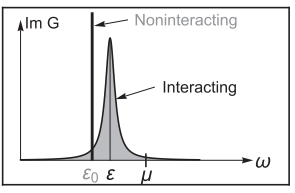
\includegraphics[scale=0.7]{figs/1p_Green_function_interacting/interacting_regime_spectral_function_one.png} }}
    \qquad
    \subfloat[\centering ]{{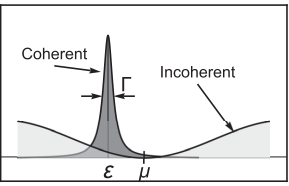
\includegraphics[scale=0.7]{figs/1p_Green_function_interacting/interacting_regime_spectral_function_two.png}}}
    \caption{\small Fig. A: Spectral function for a particle in a non-interacting system (black delta function) and of the corresponding quasiparticle after turning on interactions (gray filled curve). Notice the shift in energy and the linewidth broadening. \\
    Fig. B: Typical spectral function for a quasiparticle displaying its coherent component and the coherent background. } 
    \label{figs:1p_Green_f_(in)coh}
\end{figure}

Naturally, the full spectral function may be written as $ \mathcal{A}^{+}({\bf k}, \omega) = \mathcal{A}^{+}_{\textnormal{coh}}({\bf k}, \omega) +  \mathcal{A}^{+}_{\textnormal{incoh}}({\bf k}, \omega) $, which is schematically represented in \cref{figs:1p_Green_f_(in)coh}. The contributions from the coherent terms appear as a Lorentzian line shape, while the background arises from the incoherent part. If the quasiparticle weight vanishes, then the background only manifests itself in the spectral function. \\

The coherent terms of the spectral function have the following features:

\begin{enumerate}
    \item It has a Lorentzian profile peaked at $\varepsilon({\bf k})$. 
    \item The single-particle energies are renormalized, $\varepsilon_0 ({\bf k}) \rightarrow \varepsilon ({\bf k})$. 
    \item Its width is given by the inverse of the lifetime. 
    \item Its magnitude is proportional to the quasiparticle weight $\mathcal{Z}$, a positive number between 0 and 1. 
    \item The area under the peak has decreased, from $1$ and $\mathcal{Z}$.
\end{enumerate}

The incoherent terms, in contrasst, presents a continuum, not a peak. It must be present if $\mathcal{Z} \neq 1$, in order to satisfy the sum rule/normalization of the spectral function. A similar result is obtained for the hole spectral function, wherein $\Gamma < 0$. \\

\begin{tcolorbox}[colback=yellow, 
title = Physical Context]

Fermionic systems for which the previously laid picture holds are called Fermi liquids, its theory phenomenologically developed by Landau (1957), and in the subsequent years a microscopic formulation with the help of many-body perturbation theory was developed as well. \\

The identification and investigation of interacting fermionic systems which do not obey Fermi liquid theory is an important research area in modern many-body physics. Such non-Fermi liquids have, by definition, spectral functions which cannot be approximated by \cref{Fermi_liquids_valid_approx} and, therefore, cannot be understood in terms of a picture of non-interacting fermions. A prominent example of a non-Fermi liquid is the so-called Luttinger fermions, which occur in one-dimension.  
\end{tcolorbox}

\subsection{\textbf{Quantum Field Theory and Feynmann Rules}}

\paragraph{\textit{Perturbation theory and Feynmann Diagrams}}

In the definition of the Green function, the average values is taken with respect to the Heisenberg ground-state vector, $\ket{\psi_H}$, which is time-independent and very complicated for interacting systems, and no exact solution is achievable. The strategy is to set 

$$
    \ket{\psi_H} = \ket{\psi_I (0)} = \mathcal{S}^\dagger(t,0) \ket{\psi_I (t)},
$$

and use the time $t \rightarrow -\infty$ to interpolate the non-interacting ground state with the aid of the principle of adiabatic switching on. \\

\paragraph{The concept of Adiabaticity in Quantum Mechanics} 

The construct of adiabaticity plays an important role in quantum many-body theory, by paving a path to understand a many-body problem, even when there is only an approximate solution. \\

In order to examine the usefulness of adibaticity, consider a many-body quantum system with Hamiltonian ${\bf H} = {\bf H}_0 + {\bf H}$, for which no exact solution of its ground state $\ket{\Psi_g}$ can be obtained but the exact ground state for ${\bf H}_0$, labelled as $\ket{\Phi_g}$, is known. To connect the two systems, the ${\bf H}_0$-Hamiltonian is ever present, with ground state $\ket{\Phi_g}$, and adiabatically slowly turn on ${\bf H}'$ until the total Hamiltonian is reached. This can be done by setting 

\begin{equation}
    {\bf H}(t) = {\bf H} + \lambda(t) {\bf H}', \textnormal{ where } \lambda(t) = e^{-\eta |t|} \textnormal{ and } \eta > 0, \textnormal{ is arbitrary small, }
    \label{Adiabatic_switching_on}
\end{equation}

\begin{figure}
    \centering
    \subfloat[\centering ]{{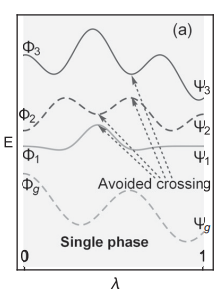
\includegraphics[scale=0.8]{figs/1p_Green_function_interacting/adiabatic_evol_no_phase_tr.png} }}
    \qquad
    \subfloat[\centering ]{{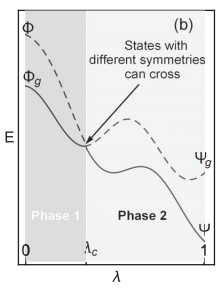
\includegraphics[scale=0.8]{figs/1p_Green_function_interacting/adiabatic_evol_phase_tr.png}}}
    \caption{\small  Fig a): Adiabatic evolution of a discrete spectrum within the symmetry subspace of the ground state. The ground state can be adiabatically evolved all the way to $\lambda = 1$, from $\ket{\Phi_g}$ to $\ket{\Psi_g}$. Fig b): Adiabatic evolution of the Hilbert space with $\lambda$. A phase transition occurs at $\lambda = \lambda_c$, where an excited state of the unperturbed Hamiltonian, with a symmetry different from that of the ground state, crosses below the ground state. } 
    \label{figs:adiabatic_evols}
\end{figure}

and varying $-\infty \leq t \rightarrow 0$. The efficacy of this approach hinges on whether $\ket{\Phi_g}$ has the same basic symmetries as $\ket{\Psi_g}$, ie. if these share the same quantum number labels. There are two possible paths for an adiabatic switching of a many-body system, diagramatically shown in figure \cref{figs:adiabatic_evols}:

\begin{enumerate}
    \item \textit{The ground-state symmetry remains invariant throughout the adiabatic evolution, } as $\lambda$ increases from 0 to 1. In such cases, the corresponding evolution of the energy spectrum, within the symmetry subspace of the ground state. In \cref{figs:adiabatic_evols}, subfigure a), a discrete spectrum with a series of avoided crossing, from $\lambda = 0$ to $\lambda = 1$, is shown. These crossings are avoided since the states have the same symmetries. The avoided crossing arise since an intersection of two levels having the same symmetry is removed because, in general, the off-diagonal matrix elements between the two states will not vanish, and thus will give rise to mutual repulsion. 
    \item \underline{The ground-state symmetry changes during the evolution due to a crossing of}
    
    \underline{ an energy level with different symmetry}, as shown in \cref{figs:adiabatic_evols}, subfigure b). In this case, it is possible for the energy levels of states with different symmetries to cross, since selection rules give vanishing matrix elements between the states, and thus prevent them from mixing. This scenarios leads to an adiabatic evolution, where a level crossing actually occurs at some $\lambda = \lambda_c$. Within such scenario, and excited state $\ket{\Phi}$ of the unperturbed Hamiltonian, with a symmetry different from that of the ground state $\ket{\Psi_g}$, may cross at $\lambda_c$ to a lower energy than the ground state, resulting in a symmetry change of the ground state. A simple example is when a ferromagnetic ground state becomes stabilized by interactions, however, in this case a continuous rotational symmetry of the spin is broken (ie. spontaneous symmetry breaking).  \\ 
\end{enumerate}

Thus, the switching-on procedure may become troublesome. Specially if it leads to instabilities at some critical value $\lambda = \lambda_c$. The presence of a $\lambda_c$ ushers a phase transition whereby the ground state changes its symmetry. If the transition is non-analytic, it signals a quantum critical transition initiated at a quantum critical point. \\

In many cases of interesent, there is no symmetry-changing phase transition as the perturbation Hamiltonian is turned on, and the procedure of adiabatic evolution can be used to turn on the interaction and to analytically evolve the ground state from $\ket{\Phi_g}$ to $\ket{\Psi_g}$. The adiabatic concept, together with the Gell-Mann-Low theorem, are key elements to perturbation theory. \\

\paragraph{Gell-Mann-Low Theorem}

\blanky \\

\begin{tcolorbox}[colback = LimeGreen, title = Historical Context]

In a 1951 seminal paper, Murray Gell-Mann and Francis Low used the adiabatic construct to establish the connection between the interacting and non-interacting Green functions, in the famous Gell-Mann-Low theorem. 

\end{tcolorbox}

The ground state $\ket{\Psi_0}$, which appears in the definition of the Green function of the interacting system, must be a time independent state in the Heisenberg picture. So far, only expectation values about the non-interacting ground state $\ket{\Phi_0}$ can be calculated. Thus, a path is needed to connect the states of the exactly solvable unperturbed Hamiltonian ${\bf H}_0$ with the ones of the full Hamiltonian. For this purpose, consider the time-dependent Hamiltonian given by \cref{Adiabatic_switching_on}, which allows for the adiabatic switching on:

\begin{itemize}
    \item For $|t|\rightarrow \infty$, the Hamiltonian reduces to ${\bf H}_0$. 
    \item At $t=0$, it becomes the interacting problem of interest.
    \item In the $\eta \rightarrow 0$-limit, the interaction is switched on adiabatically.
\end{itemize}

The scattering operator, in this context, is thus defined as 

\begin{equation}
    \mathcal{S}_{\eta}(t, t_0) = \sum_{n = 0}^{\infty} \frac{1}{n!} (-i)^{n} \int_{t_0}^{t} dt_1 \cdots \int_{t_0}^{t} dt_n \blanky e^{-\eta (|t_1| + \cdots + |t_n|)} \mathcal{T} [{\bf H}_{I}(t_1) \cdots {\bf H}_{I}(t_n)].
\end{equation}

As $t_0 \rightarrow - \infty$, the effect of the interaction vanishes and the problem reduces to that of the unperturbed Hamiltonian, 

$$
    t_0 \rightarrow -\infty \Longleftrightarrow \left\{\begin{array}{cc}
         {\bf H}_0 \ket{\Psi_0} = E^{(0)} \ket{\Psi_0}  \\
         \ket{\Psi_I(t_0)} \rightarrow \ket{\Psi_0}. 
    \end{array}\right.
$$

Now, recall the relation among state vector in different pictures, 

$$
    \ket{\Psi_H} = \ket{\Psi_S(t=0)} = \ket{\Psi_I (t=0)},
$$

where $t=0$ corresponds to the fully interacting Hamiltonian. In particular, the following relation between the Heisenberg and interaction state vectors is found 

$$
    \ket{\Psi_H} = \ket{\Psi_I (0)} = \mathcal{S}_{\eta}(0, - \infty) \ket{\Psi_0}. 
$$

The previous equation gives the relationship between the eigenstates of the non-interacting system with those of the fully interacting one, albeit via the adiabatic switching process. Then, the following theorem arises \\

\begin{theorem} \textbf{\textnormal{Gell-Mann-Low theorem}}

In the absence of any symmetry breaking transition, and in the $(\eta \rightarrow 0)$-limit, $\mathcal{S}_{\eta} \rightarrow \mathcal{S}_I$, and provides the right solution. To be more precise, let $\ket{\Psi_0}$ be an eigenstate of the unperturbed Hamiltonian ${\bf H_0}$ with energy $E^{(0)}$, and consider the interacting Hamiltonian given by

$$
    {\bf H} = {\bf H} + g e^{-\eta |t|} {\bf H}',
$$

which effectively interpolates between ${\bf H}$ and ${\bf H}_0$ in the limit $\eta \rightarrow 0$ and $|t|\rightarrow 0$. Let $\mathcal{S}_{\eta}$ denote the evolution operator in the interaction limit. Then, in the $(\eta \rightarrow 0)$-limit,

$$
    \ket{\Psi_{\eta}^{(\pm)}} = \frac{\mathcal{S}(0, \pm\infty) \ket{\Psi_0}}{\bra{\Psi_0} \mathcal{S}(0, \pm\infty) \ket{\Psi_0}},
$$

exists, is well defined with the $ \ket{\Psi_{\eta}^{(\pm)}}$-states being the eigenstates of the full Hamiltonian.

\end{theorem}

\begin{proof}

In effect, let the coupling constant be $g = e^{\eta \theta}$ and consider the Dyson expansion of the evolution operator. From Schr\"odinger's equation for the time evolution operator, it is known that 

$$
    i \partial_{t_1} \mathcal{S}_{\eta}(t_1,t_2) = {\bf H} \mathcal{S}_{\eta}(t_1,t_2), \textnormal{ with } \mathcal{S}_{\eta}(t_2,t_2) = \textnormal{id}, 
$$

and the adjoint Schr\"odinger equation establishes that 

$$
-i \partial_{t_1} \mathcal{S}_{\eta}(t_1,t_2) = \mathcal{S}_{\eta}(t_1,t_2) {\bf H}(t_1). 
$$

Then, formally 

$$
    \mathcal{S}_{\eta}(t_1,t_2) = \textnormal{id} - i \int_{t_2}^{t_1}dt' \blanky ({\bf H}_0 + e^{-\eta (|t'| - \theta)} {\bf H}') \mathcal{S}_{\eta}(t',t_2).
$$


Then, for $t_2 \leq t_1 \leq 0$ and with $\tau = t' + \theta$, it follows that 

\begin{equation}
    \begin{split}
        \mathcal{S}_{\eta}(t_1,t_2) = \textnormal{id} - i \int_{\theta + t_2}^{\theta + t_1}dt' \blanky ({\bf H}_0 + e^{\eta \tau} {\bf H}') \mathcal{S}_{\eta}(\tau - \theta,t_2) \\
        \Rightarrow \partial_{\theta} \mathcal{S}_{\eta}(t_1,t_2) \equiv \eta \partial_{g} \mathcal{S}_{\eta}(t_1,t_2) =& \partial_{t_1} \mathcal{S}_{\eta}(t_1,t_2) + \partial_{t_2}\mathcal{S}_{\eta}(t_1,t_2) \\
        &= {\bf H}(t_1) \mathcal{S}_{\eta}(t_1,t_2) - \mathcal{S}_{\eta}(t_1,t_2) {\bf H}(t_2).
    \end{split}
    \label{Gell_Mann_Low}
\end{equation}

The corresponding equation in the interaction picture can be obtained from the previous equation by pre-multiplying both sides with $e^{i {\bf H} t_1}$ and post-multiplying with $e^{i {\bf H} t_2}$ and using the definition of the interaction picture, namely that 

$$
    \mathcal{S}_{\eta, I}(t_1,t_2) = e^{i {\bf H_0} t_1} \mathcal{S}_{\eta}(t_1,t_2) e^{i {\bf H_0} t_2}. 
$$

The other case, in which $t_2 \geq t_1 \geq 0$, can be obtained in a similar fashion, yielding an additional global minus sign in front of the commutator. The mixed-sign case is not of interest here. Then, using the definition of the $\ket{\Psi_{\eta}^{(\pm)}}$ and employing \cref{Gell_Mann_Low}

\begin{equation}
    \begin{split}
        &\bigg({\bf H}_{\eta}(t=0) - E_0 \pm i \eta g \partial_{g} \bigg) \mathcal{S}_{\eta, I}(0,\pm \infty) \ket{\Psi_0} = 0. \\
        &\Rightarrow \mp i \eta g \partial_{g} \mathcal{S}_{\eta, I}(0,\pm \infty) \ket{\Psi_{\eta}^{(\pm)}}= ({\bf H}_{\eta} - E_0)  \mathcal{S}_{\eta, I}(0,\pm \infty) \ket{\Psi_{\eta}^{(\pm)}}\\
        &\Rightarrow \mp i \eta g \partial_{g} \ket{\Psi_0}= \frac{({\bf H} - E_0) \mathcal{S}_{\eta}(t_1,t_2) \ket{\Psi_0} }{ \bra{\Psi_0} \mathcal{S}_{\eta}(t_1,t_2) \ket{\Psi_0}} - \frac{\mathcal{S}_{\eta}(t_1,t_2) \ket{\Psi_0}}{ \bra{\Psi_0} \mathcal{S}_{\eta}(t_1,t_2) \ket{\Psi_0}} \bra{\Psi_0} ({\bf H} - E_0) \mathcal{S}_{\eta}(t_1,t_2) \ket{\Psi_0}  \\
\\
\Rightarrow \mp i \eta g \partial_{g} \ket{\Psi_0} &= ({{\bf H}} - E_0) \ket{\Psi_{\eta}^{(\pm)}} -  \bra{\Psi_{\eta}^{(\pm)}} \bra{\Psi_0} {{\bf H}} - E_0  \ket{\Psi_{\eta}^{(\pm)}} \\
&= [{{\bf H}} -\mathcal{E}^{(\pm)}] \ket{\Psi_{\eta}^{(\pm)}},
    \end{split}
\end{equation}

where $\mathcal{E}^{(\pm)} = E_0 + \bra{\Psi_0} {{\bf H}} - {{\bf H}}_0  \ket{\Psi_{\eta}^{(\pm)}}$. In the $\eta \rightarrow 0^+$-limit, by assumption, $g \partial_{g} \ket{\Psi_{\eta}^{(\pm)}}$ is finite. Then, it is clear that $\ket{\Psi_{\eta}^{(\pm)}}$ is an eigenstate of the full Hamiltonian, completing the proof. 

\end{proof}

\blanky \\

\paragraph{One-particle Green functions as a power series in the interaction}

The Gell-Mann-Low theorem connects the eigenstates of the non-interacting system with those of the fully interacting one, with the aid of the interaction picture. The Heisenberg operators, appearing in the Green function, remain to be related to those in the corresponding interaction picture. \\

To that end, consider the relationship between operators in the Heisenberg and interaction pictures,

\begin{equation}
    {\bf O}_{H}(t) = e^{i {\bf H} t} {\bf O}_{S} e^{-i {\bf H} t} = e^{i {\bf H} t} e^{-i {\bf H}_0 t} {\bf O}_{I} e^{i {\bf H}_0 t} e^{-i {\bf H} t}.
\end{equation}

Furthermore, the states in the interaction picture are given by 

\begin{equation}
    \ket{\Psi_I(t)} = e^{i{\bf H}_0 t} e^{-i {\bf H}t} \ket{\Psi_I(0)} = \mathcal{S}_{I}(t,0) \ket{\Psi_I(0)}.
\end{equation}

Then, 

\begin{equation}
    {\bf O}_{H}(t) = \mathcal{S}_{I}(0,t) {\bf O}_{I}(t) \mathcal{S}_{I}(t,0). 
\end{equation}

With these ingredients, the product of two Heisenberg operators, in the interaction picture, reads

\begin{equation}
    \begin{split}
        {\bf O}_{H}(t) {\bf O}_{H}(t_1) =& \mathcal{S}_{I}(0,t) {\bf O}_{I}(t) \mathcal{S}_{I}(t,0)  \mathcal{S}_{I}(0,t_1) {\bf O}_{I}(t_1) \mathcal{S}_{I}(t_1,0) \\
        &= \mathcal{S}_{I}(0,t) {\bf O}_{I}(t) \mathcal{S}_{I}(t,t_1) {\bf O}_{I}(t_1) \mathcal{S}_{I}(t_1,0).
    \end{split}
\end{equation}

Then, the Green function in terms of interaction-picture operators reads

\begin{equation}
\begin{split}
    i \mathfrak{G}(x; x') &= \bra{\Psi_H} \mathcal{T} [\psi_{H}(x) \psi^\dagger_{H}(x')] \ket{\Psi_H} \\
    &= \frac{\bra{\Phi_0} \mathcal{S}_I(\infty, 0) \mathcal{T} [\mathcal{S}_I(0, t) \psi_{I}(x) \mathcal{S}_I(t, t') \psi_{I}(x') \mathcal{S}_I(t', 0) ] \mathcal{S}_I(0, -\infty)\ket{\Phi_0}}{\bra{\Phi_0} \mathcal{S}_I(\infty, 0)\mathcal{S}_I(0, -\infty)\ket{\Phi_0}},
\end{split}
\end{equation}

where $x \equiv ({\bf x}, t, \sigma)$ for compactness. The $(\psi_H, \psi_H^\dagger)$-Heisenberg operators have been replaced by their interaction-picture conterparts, which simply evolve under the action of the unperturbed Hamiltonian ${\bf H}_0$. The ground state of the interaction problem $\ket{\Psi_0}$ has been replaced by the non-interacting one, $\ket{\Phi_0}$. Furthermore, since the evolution operations $\mathcal{S}$ form a semigroup, all evolution operators in the preceding equation can be combined into a single $\mathcal{S}$, for the time-ordering operator takes care of the proper time ordering anyhow, thus yielding 

\begin{equation}
\begin{split}
     i \mathfrak{G}^{\sigma \sigma'}({\bf x}, t; {\bf x}', t') &= \frac{\bra{\Phi_0}  \mathcal{T} [\mathcal{S}_I(-\infty, \infty) \psi_{I \sigma}({\bf x}, t)\psi_{I \sigma'}({\bf x}', t')]\ket{\Phi_0}}{\bra{\Phi_0} \mathcal{S}_I(\infty, -\infty)\ket{\Phi_0}} \\
     &= \sum_{n=0}^{\infty} \frac{1}{n!} (-i)^n \int_{-\infty}^{\infty} dt_1 \cdots \int_{-\infty}^{\infty} dt_n \blanky \frac{\bra{\Phi_0} \mathcal{T} [{\bf H}_{I}(t_1) \cdots {\bf H}_{I}(t_n) \psi_{I \sigma}({\bf x}, t)\psi_{I \sigma'}({\bf x}', t')]\ket{\Phi_0}}{\bra{\Phi_0} \mathcal{S}_I(\infty, -\infty)\ket{\Phi_0}},
     \label{GF_perturbation_exp}
\end{split}
\end{equation}

where the one-particle Green function is now explicitly written as an expansion in powers of the perturbation ${\bf H}_I$. For this reformulation to be useful, a method is needed to mitigate taking expectation values of large numbers of operators in a non-interacting sytem. This procedure is systematized with the application of Wick's theorem and simplified with the aid of Feynmann diagrams. \\

\paragraph{\textit{Wick's Theorem: Normal ordering and contractions}}

In the preceding identity for the one-particle Green function, the arraying of interaction Hamiltonians is fixed by time ordering. However, as the interaction Hamiltonian contains creation and annihilation operators, it is convenient to move all annihilation operators to the right, where these can eliminate particles. This ordering is called the \textit{normal ordering}. Furthermore, observables have zero-expectation values in the vacuum state, it is convenient to construct them in normal order, with creation operators on the left of destruction operators. Wick's theorem provides a way to go from time-ordered to normal-ordered products, which is valid when the expectation values are with respect to a Hamiltonian that is quadratic in fermionic (bosonic) operators. \\

Recall from the study of superfluidity phenomenom that the Bogoliubov canonical transformation generated new non-interacting quasiparticles from the original interacting bosons, and the emerging ground state acted as a vacuum state for the new quasiparticles. 
In many physical situations, the ground state $\ket{\Psi_g}$, of some incipient effective Hamiltonian, will be taken to be the reference vacuum state. Such a state is filled with both particles and quasiparticles, and the effective Hamiltonian is expressed in a basis of canonical operators $\bigg\{({\bm \alpha}_{a}, {\bm \alpha}^\dagger_{a})\bigg\}_{a = 1}$, where 

\begin{align}
    {\bm \alpha}_{a} \ket{\Psi_g} &= 0, & \bra{\Psi_g} {\bm \alpha}_{a}^\dagger = 0,
\end{align}

where this action only holds for such systems, but not for the other creation and annihilation operators associated with the system. \\

\begin{tcolorbox}[colback = yellow, title = Physical Context]

In order to bring light upon these ideas, consider the non-interacting ground state $\ket{\Phi_0}$, describing the Fermi sea. Then, the field operators are given in terms of the canonical particle-hole transformation,

\begin{equation}
    \psi({\bf x}) = \sum_{{\bf k} \sigma} \phi_{{\bf k} \sigma} {\bf c}_{{\bf k} \sigma} = \left\{\begin{array}{cc}
       \sum_{{\bf k} \sigma} \phi_{{\bf k} \sigma}({\bf x}) {\bf d}_{{\bf k} \sigma} = \phi^{(-)}({\bf x}) & \textnormal{ if $k > k_F$ annihilates particles}{} \\
       \sum_{{\bf k} \sigma} \phi_{{\bf k} \sigma}({\bf x}) {\bf h}_{-{\bf k} \sigma} = \phi^{(+)}({\bf x}) & \textnormal{ if $k < k_F$ create holes }{}
    \end{array}\right.,
\end{equation}

then 

\begin{align}
    \phi^{(-)}({\bf x}) \ket{\Phi_0} &= 0, & \phi^{(+)^\dagger}({\bf x}) \ket{\Phi_0} &= 0.
\end{align}

The preceding relations indicate that $(\phi^{(-)}, \phi^{(+)\dagger})$ are annihilation parts, while $(\phi^{(+)}, \phi^{(-)\dagger})$ are the creation operators. 

\end{tcolorbox}

The following discussion will be restricted to 
fermionic operators in a non-interacting system. 

\begin{definition}

Consider a product of operators ${\bf A}_i^{\pm}$ is normally ordered if all the ${\bf A}_i^{-}$-operators are on the right of the ${\bf A}_i^{+}$-operators, i.e.

$$
    {\bf A}_1^{+} \cdots {\bf A}_k^{+} {\bf A}_1^{-} \cdots {\bf A}_n^{-}.
$$

\end{definition}

The usefulness of this definition is that the expectation value on the ground state of a normally ordered operator product is always zero. \\

It is clear that any product of operators ${\bf A}_1 \cdot {\bf A}_n$ can be written as a sum of normally ordered terms. In effect, every local operator can be written as ${\bf A}_i^{+} + {\bf A}_i^{-}$, thus yielding $2^n$ terms. In each term, the components ${\bf A}_i^{-}$ are brought to the right by succesive anticommutation, yielding the desired result. Wick's theorem is an efficient answer to this particular problem: to write a product $\prod_{i} {\bf A}_i$ as a sum of normally ordered terms. The theorem is an extremely useful operator identity, with important corollaries. \\

\begin{definition}[Normal Ordering]
    The normal-ordering operator, $\bm{\mathcal{N}}$ brings a generic product into a normal form. If a product of operators contains $k$ ${\bf A}_i^+$-factors mixed with $n-k$ ${\bf A}^-_i$-factors, it action is given by 
    
    \begin{equation}
        \bm{\mathcal{N}} [{\bf A}_i^{(\pm)} \cdots {\bf A}_n^{(\pm)}] = (\pm 1)^{P} {\bf A}_{i_1}^{+} \cdots {\bf A}_{i_k}^{+} \cdots {\bf A}_{i_n}^{-}, 
    \end{equation}
    
    where $P$ is the permutation which brings the $(1, \cdots,n)$-sequence to its normal ordered $(i_1, \cdots, i_n)$-sequence. \\
\end{definition}

At first glance, it may seem that the normal ordering is ambiguous, since the (+)-operators and $(-)$-operators can be given in different orders. However, the different expressions are actually the same operator, since ${\bf A}^+$-operators anticommute among themselves, with the same being true for the ${\bf A}^-$-operators. For example, $\bm{\mathcal{N}}[{{\bf A}_1^+ {\bf A}_2^+}] = {{\bf A}_1^+ {\bf A}_2^+} = - {{\bf A}_2^+ {\bf A}_1^+}$. Now, any product $\prod_i {\bf A}_i$ can be written as a sum of normally ordered terms. 

\begin{tcolorbox}[colback = Bittersweet, title = Example]

Consider for example a product of two operators, 

\begin{equation*}
    \begin{split}
        {\bf A}_1 {\bf A}_2 &= ({\bf A}_1^+ + {\bf A}_1^-)({\bf A}_2^+ + {\bf A}_2^-) \\
        &= {\bf A}_{1}^{+} {\bf A}_{2}^{+} + {\bf A}_{1}^{-} {\bf A}_{2}^{+} + {\bf A}_{1}^{+} {\bf A}_{2}^{-} + {\bf A}_{1}^{-} {\bf A}_{2}^{-} \\
        &= \bm{\mathcal{N}} [{\bf A}_1 {\bf A}_2] + \{{\bf A}_1^-, {\bf A}_2^+\}.
    \end{split}
\end{equation*}

The vanishing of the expectation value of a normally ordered product implies 

\begin{equation*}
    \{{\bf A}_1^-, {\bf A}_2^+\} = \bra{\Psi_g} {\bf A}_1 {\bf A}_2 \ket{\Psi_g},
\end{equation*}

which is a c-number, the \underline{contraction} of the two operators, denoted ${\bf A}_1^c {\bf A}_2^c$. 

\end{tcolorbox}

Using the previous example:

\begin{definition}[Contraction]
     
    The contraction of two operators, where a product of $n'$ operators is inserted between them, may be defined by 
    
    \begin{equation}
        {\bf A}_1^c ({\bf A}_{1'} \cdots {\bf A}_{n'}) {\bf A}_2^c = (-1)^{n'}   {\bf A}_1^c {\bf A}_2^c ({\bf A}_{1'} \cdots {\bf A}_{n'}).
    \end{equation}
     
\end{definition}

Wick's theorem provides a computationally efficient way for calculating operator contractions, by mapping it to a purely combinatorial problem. 

\begin{theorem}Wick's theorem \\

Consider a product of $n$ operators, then the following equality holds:

\begin{equation}
    {\bf A}_1 \cdots {\bf A}_n = \bm{\mathcal{N}}[1\cdots n] + \sum_{c} \bm{\mathcal{N}}[\cdots i^c \cdots j^c \cdots n] + \sum_{c, d} \bm{\mathcal{N}}[\cdots i^c \cdots r^d \cdots j^c \cdots s^d \cdots n] + \cdots,
\end{equation}

where the first sum is performed over single contractions of pairs, the second sum is performed over double contractions and so on. If $n$ is even, the result consists only of products of contractions (c-numbers).

\end{theorem}

Some important consequences of Wick's theorem readily follow, 

\begin{remark}
    As a general rule, the expectation value of a product of destruction and creation operators. Particle number conservation thus requieres that the number of destruction operators equals that of creators.
\end{remark}

\begin{corr}

The following identity can be proved from Wick's theorem\footnote{

\begin{tcolorbox}[colback = Bittersweet, title = Example]

Using the previous corollary, it is trivial that 

\begin{equation*}
    \bra{\Psi_g} 1234 \ket{\Psi_g} = \langle 12 \rangle \langle 34 \rangle - \langle 13 24 \rangle + \langle 14 \rangle \langle 23 \rangle.
\end{equation*}

\end{tcolorbox}

},

\begin{equation}
    \bra{\Psi_g} {{{\bf A}}}_1 \cdots {{\bf A}}_{2n} \ket{\Psi_g} = \sum_{\mathcal{P}_2} (-1)^{P} \langle {{\bf A}}_{i_1} {{\bf A}}_{j_1} \rangle \cdots \langle {{\bf A}}_{i_n} {{\bf A}}_{j_n} \rangle, {\begin{array}{cc}
         \textnormal{ where the sum is performed over the set $\mathcal{P}_2$ of}  \\
         \textnormal{ partitions of $1, \cdots, 2n$ into sets of } \\
         \textnormal{ pairs $\{(i_1, j_1), \cdots, (i_n, j_n)\}$ with $(i,j) \sim (j,i)$} \\
         \textnormal{ belonging to the same equivalency class.}
    \end{array}}
\end{equation}

\end{corr}

\blanky \\
An important variation of Wick's theorem deals with the normal-ordering of a time-ordered product, via a $\bm{\mathcal{T}}$-contraction operator. 

\begin{theorem}

Consider a product of two-operators. Then, its time-ordered product can be written as 

\begin{equation}
    \mathcal{T} {{\bf A}}_{i}(t_i) {{\bf A}}_{j}(t_j) = \bm{\mathcal{N}}[{{\bf A}}_{i}(t_j) {{\bf A}}_{j}(t_i)] + \overbrace{{{\bf A}}_{i}(t_i) {{\bf A}}_{j}(t_j)}, 
\end{equation}

then a $\bm{\mathcal{T}}$(time ordered)-contraction is defined as 

\begin{equation}
    \overbrace{{{\bf A}}_{i}(t_i) {{\bf A}}_{j}(t_j)} = \bra{\Psi_g} \mathcal{T} {{\bf A}}_{i}(t_i) {{\bf A}}_{j}(t_j) \ket{\Psi},
\end{equation}

\end{theorem}

\begin{remark}
    The $\bm{\mathcal{T}}$-contraction of two-operators is such that 
    
    \begin{equation}
        \overbrace{{{\bf A}}_{i}(t_i) (\cdots ) {{\bf A}}_{j}(t_j)} = (-1)^k \overbrace{{{\bf A}}_{i}(t_i) {{\bf A}}_{j}(t_j)} ()\cdots).
    \end{equation}
\end{remark}

\begin{remark}
    The $\bm{\mathcal{T}}$-contractions have a new property, not shared by ordinary contractions,
    
    \begin{equation}
        \overbrace{{{\bf A}}_{i}(t_i) {{\bf A}}_{j}(t_j)} = - \overbrace{{{\bf A}}_{j}(t_j) {{\bf A}}_{i}(t_i)}.
    \end{equation}
\end{remark}

\begin{remark}

From the previous definitions and remarks, the following explicit expressions can be given, 

\begin{equation} \begin{split}
    \overbrace{\psi(t_1) \psi^\dagger(t_2)} =& \bigg \langle \mathcal{T} \psi(t_1) \psi^\dagger(t_2) \bigg \rangle \\
    &= i \mathfrak{G}^{(0)}(1,2)
\end{split}, \blanky \blanky \blanky \blanky \begin{split}
    \overbrace{\psi(t_1) \psi(t_2)} =& \bigg \langle \mathcal{T} \psi(t_1) \psi(t_2) \bigg \rangle \\
    &= i \mathfrak{F}^{(0)}(1,2)
\end{split}, \blanky \blanky \blanky \blanky \begin{split}
    \overbrace{\psi^\dagger(t_1) \psi^\dagger(t_2)} =& \bigg \langle \mathcal{T} \psi^\dagger(t_1) \psi^\dagger(t_2) \bigg \rangle \\
    &= i \mathfrak{F}^{(0)\dagger}(1,2).
\end{split}
\end{equation}
    
\end{remark}

For systems where $\ket{\Psi_g}$ has a definite number of particles, the anomalous correlators $\mathfrak{F}^{(0)}, \mathfrak{F}^{(0)\dagger}$ are zero. They are non-zero, for example, in the Bardeen-Cooper-Schrieffer theory. \\

\subsubsection{\textbf{Feynmann Diagrams}}

Consider the perturbation expansion of the Green function, given by \cref{GF_perturbation_exp} and consider only terms linear on the interaction Hamiltonian ${\bf H}_I$, ie. 

\begin{equation}
    i \mathfrak{G}_{\sigma \sigma'} \rightarrow i \mathfrak{G}_{\sigma \sigma'}^{(0)} + i \mathfrak{G}_{\sigma \sigma'}^{(1)}, \textnormal{ with } \begin{array}[cc]
        i \mathfrak{G}_{\sigma \sigma'}^{(1)} \propto -i \int_{\mathds{R}} dt \blanky \bra{\Psi_0} \mathcal{T} [{\bf H}_I(t_1) \psi_{I \sigma}({\bf x}, t) \psi^\dagger_{I \sigma'}({\bf x}', t')] \ket{\Psi_0} \\
        \\
        {\bf H}_I = \frac{1}{2} \int_{\mathds{R}^6} d{\bf x}_1 d{\bf x}_2 \blanky \psi^\dagger_{\sigma_1}({\bf x}_1) \psi^\dagger_{\sigma_2}({\bf x}_2) V(|{\bf x}_1 - {\bf x}_2|) \psi_{\sigma_2'}({\bf x}_2) \psi_{ \sigma_1'}({\bf x}_1).
    \end{array}  
    \label{GreenFunc_expansion_Hamiltonians}
\end{equation}

Consider the interaction of the form 

$$
    V_{\sigma_1\sigma'_1}^{\sigma_2\sigma'_2}({{\bf x}}_1, t_1; {{\bf x}}_2, t_2) = V(|{{\bf x}}_1 - {{\bf x}}_2|) \psi_{\sigma_2'}({{\bf x}}_2) \delta(t_1-t_2) \delta_{\sigma_1\sigma'_1}^{\sigma_2\sigma'_2},
$$

then

\begin{equation}
    \begin{split}
        i \mathfrak{G}_{\sigma \sigma'}^{(1)} \propto - \frac{i}{2} \sum_{{\substack{\sigma_1, \sigma'_1 
         \\ \sigma_2, \sigma_2'}}}
        \int_{\mathds{R}^8} d^4x_1 d^4x_2 V_{\sigma_1\sigma'_1}^{\sigma_2\sigma'_2}(x_1, x_2) \bra{\Psi_0} \mathcal{T} \bigg[ \psi_{\sigma_1}^\dagger(x_1) \psi_{\sigma_2}^\dagger(x_2) \psi_{\sigma'_2}(x_2) \psi_{\sigma'_1}(x_1) \psi_{\sigma}(x) \psi^\dagger_{\sigma'}(x') \bigg] \ket{\Psi_0}
        \label{first_order_perturb_Green_function}
    \end{split}
\end{equation}

The problem of interacting electrons has been reduced to determining expectation values of its non-interacting counterparts. Now, Wick's theorem must be applied by considering all possible pair contractions. Each particle emerging from a creation operator in the previous equation, must be destroyed by an annihilation operator. Thus, every creation operator can be paired to an annihilation operator, keeping in mind the following simplifying points to obtain the final expression of the first-order Green function in terms of the free Green functions:

\begin{itemize}
    \item the ground state is that of ${\bf H}_0$, 
    \item the operators now have the form
          $$
            \psi_\sigma^\dagger({\bf x},t) = e^{i {\bf H}_0 t} \psi_{S \sigma}^\dagger({\bf x}) e^{-i {\bf H}_0 t}.
          $$
          
          For eigenstates of the unperturbed Hamiltonian representing a crystalline solid, these can be written as 
          
           $$
            e^{i {\bf H}_0 t} {\bf c}_{n {\bf k} \sigma}^\dagger e^{-i {\bf H}_0 t} \rightarrow e^{i \varepsilon_{n {\bf k}} t}{\bf c}_{n {\bf k} \sigma}^\dagger.
          $$
          
    \item An injected electron in the $\ket{n {\bf k} \sigma}$ of a non-interacting system must be removed from the same state, since it evolves in time unperturbed. This allows for the insertion of $\ket{\Psi_0}\bra{\Psi_0}$ between pairs of creation and annihilation operators to obtain
    
    $$
        \bra{\Psi_0} {{\bf c}}_{n {{\bf k}} \sigma}(t) {{\bf c}}_{n {{\bf k}} \sigma}^\dagger(t_1) \ket{\Psi_0},
    $$
    
    which is just the non-interacting single-particle Green function. This procedure can be generalized to all creation and annihilation operators a Green function contains, for they represent non-interacting systems. This is a direct consequence of Wick's theorem. 
    
\end{itemize}

All in all, this procedures yield a total of six terms in the first-order Green function, given in \cref{first-order perturb Green function}, which can be obtained from all possible pair-wise contractions of a creation operator with an annihilation operator, yielding 

\begin{equation}
    \begin{split}
        \bra{\Psi_0} &\mathcal{T} \bigg[ \psi_{\sigma_1}^\dagger(x_1) \psi_{\sigma_2}^\dagger(x_2) \psi_{\sigma'_2}(x_2) \psi_{\sigma'_1}(x_1) \psi_{\sigma}(x) \psi^\dagger_{\sigma'}(x') \bigg] \ket{\Psi_0} =\\
        &= \bigg({\wick{ \c2\psi_{\sigma_1}^\dagger(x_1) \c1 \psi_{\sigma_2}^\dagger(x_2) \c1 \psi_{\sigma'_2}(x_2) \c2\psi_{\sigma'_1}(x_1)} 
        }-{\wick{ \c1\psi_{\sigma_1}^\dagger(x_1) \c2 \psi_{\sigma_2}^\dagger(x_2) \c1 \psi_{\sigma'_2}(x_2) \c2\psi_{\sigma'_1}(x_1)} 
        }\bigg) \wick{\c  \psi_{\sigma}(x) \c\psi^\dagger_{\sigma'}(x') } \\
        &\blanky \blanky \blanky+ \wick{
        \c3 \psi_{\sigma_1}^\dagger(x_1) 
        \c2 \psi_{\sigma_2}^\dagger(x_2) 
        \c1 \psi_{\sigma'_2}(x_2) 
        \c2 \psi_{\sigma'_1}(x_1) 
        \c3 \psi_{\sigma}(x) 
        \c1 \psi^\dagger_{\sigma'}(x') } - \wick{\c3 \psi_{\sigma_1}^\dagger(x_1)  \c1 \psi_{\sigma_2}^\dagger(x_2)  \c1 \psi_{\sigma'_2}(x_2) \c2 \psi_{\sigma'_1}(x_1) \c3 \psi_{\sigma}(x) \c2 \psi^\dagger_{\sigma'}(x') } \\
        &\blanky \blanky \blanky + \wick{\c1 \psi_{\sigma_1}^\dagger(x_1) \c3 \psi_{\sigma_2}^\dagger(x_2) \c1 \psi_{\sigma'_2}(x_2) \c2 \psi_{\sigma'_1}(x_1) \c3 \psi_{\sigma}(x) \c2 \psi^\dagger_{\sigma'}(x') } - \wick{\c1 \psi_{\sigma_1}^\dagger(x_1) \c3 \psi_{\sigma_2}^\dagger(x_2) \c2 \psi_{\sigma'_2}(x_2) \c1 \psi_{\sigma'_1}(x_1) \c3 \psi_{\sigma}(x) \c2 \psi^\dagger_{\sigma'}(x') } \\
        &= i{\mathfrak{G}_{\sigma \sigma'}^{(x,x'); (0)}} \bigg(i{\mathfrak{G}_{\sigma_1 \sigma'_1}^{(x_1, x_1); (0)}} i{\mathfrak{G}_{\sigma_2 \sigma'_2 }^{(x_2,x_2); (0)}} - i{\mathfrak{G}_{\sigma'_1\sigma_2}^{(x_1, x_2); (0)}} i{\mathfrak{G}_{\sigma'_2 \sigma_1}^{(x_2, x_1); (0)}}\bigg)  \\
        & \blanky \blanky \blanky + i{\mathfrak{G}_{\sigma \sigma_1}^{(x,x_1); (0)}}\bigg(  i{\mathfrak{G}_{\sigma'_1 \sigma_2}^{(x_1,x_2); (0)}} i{\mathfrak{G}_{\sigma'_2\sigma_2}^{(x_2, x'); (0)}} -  i{\mathfrak{G}_{\sigma'_1 \sigma'}^{(x_1, x'); (0)}} i{\mathfrak{G}_{\sigma'_2 \sigma_2}^{(x_2, x_2); (0)}} \bigg) \\
        & \blanky \blanky \blanky + i{\mathfrak{G}_{\sigma \sigma_2}^{(x, x_2);(0)}} \bigg(i{\mathfrak{G}_{\sigma'_2 \sigma_1}^{(x_2, x_1);(0)}}
        i{\mathfrak{G}_{\sigma'_1 \sigma'}^{(x_1, x');(0)}} - 
        i{\mathfrak{G}_{\sigma'_2 \sigma'}^{(x_2, x');(0)}}
        i{\mathfrak{G}_{\sigma_1' \sigma_2}^{(x_1, x_1);(0)}}\bigg) 
    \end{split}
    \label{first_order_contractions}
\end{equation}

The, using Wick's theorem, each term in the perturbation expansion can be expressed as a product of non-interacting Green functions, which is the general methodology behind perturbation theory. \\

\paragraph{Equal-Time operators}

In the previous calculation, the Green functions are ambiguous, since these represent contractions of creation and annihilation operators at equal times with the time-ordered product being undefined at equal times. Moreover, \cref{NR_GF_Jellium_like_model} has a discontinuity at equal times $t=t'$. Consequently, taking this limit from either side will yield different results. However, \cref{first_order_perturb_Green_function} shows that the the operators of ${\bf H}_I$ come in sets of four having identical times and a term such as ${\mathfrak{G}^{(x_1, x_1);(0)}}$ arising from a contraction of two fields within the perturbation Hamiltonian, where they appear in the form of $\psi^\dagger(x)\psi(x)$ with the adjoint field always occurring to the left of the field, 

$$
    {\bf H}_I \propto \psi_{\sigma_1}^\dagger ({\bf x}_1) \psi_{\sigma_2}^\dagger ({\bf x}_2) \psi_{\sigma'_2} ({\bf x}_2) \psi_{\sigma'_1} ({\bf x}_1) \rightarrow 
    \psi_{\sigma_1}^\dagger ({\bf x}_1)  \psi_{\sigma'_1} ({\bf x}_1) \psi_{\sigma_2}^\dagger ({\bf x}_2) \psi_{\sigma'_2} ({\bf x}_2), \quad {\bf x}_1 \neq {\bf q}_2.
$$

When this term is replaced in the propagators, the backward time propagation introduces a (-1)-factor for fermions. Therefore, Green functions at equal times for fermionic systems are to interpreted as follows

\begin{equation}
    \begin{split}
        \mathfrak{G}_{\sigma \sigma'}^{(0)}(x,x) =& \lim_{t' \rightarrow t} \bra{\Psi_0} \psi_{\sigma}({\bf x}, t)  \psi^\dagger_{\sigma'}({\bf x}, t') \ket{\Psi_0} \\
        &= - \bra{\Psi_0} \psi^\dagger_{\sigma'}({\bf x}) \psi_{\sigma}({\bf x}) \ket{\Psi_0} = - \delta_{\sigma \sigma'} \frac{n^{(0)}({\bf x)}}{2s+1},
    \end{split}
\end{equation}

for fermionic systems of $s$-spin, where $n^{(0)}({\bf x})$ is the electron density in the non-interacting system, which may be different from $n({\bf x})$ of the interacting system. For a uniform system, like the jellium, they coincide. \\

As a general rule, if two operators occur at equal time, they should be normal ordered. Operationally, this means that, when encountering Green functions of the form $\mathfrak{G}^{(0)}({\bf x}, {\bf x}'; t = 0)$, these should be interpreted as 

\begin{equation}
    \mathfrak{G}^{(0)}({\bf x}, {\bf x}'; t = 0) \equiv \lim_{\epsilon^{-}} \mathfrak{G}_{\sigma \sigma'}^{(0)}({\bf x}, {\bf x}'; t + \epsilon)
\end{equation}

\subsubsection{The Feynmann Rules}

The Feynmann rules allows for the calculation of the $n$-th-order term in the perturbation expansion of the Green function, which can be formulated in both direct space and in momentum space. The rules read

\begin{itemize}
    \item Draw all topologically distinct connected diagrams with $n$ interaction (wavy) lines $V$ and $2n+1$ Green function $\mathfrak{G}^{(0)}$ solid lines. 
    \item Each wavy line corresponds to the interaction written in \cref{first_order_perturb_Green_function} (its Fourier transform in $({\bf k}-\omega)$-basis.
    \item Vertex and line labelling: 
    \begin{itemize}
        \item ${\bf x -t}$-basis: Each vertex is labelled by a point in spacetime $x_i$; each solid line represents a Green function $\mathfrak{G}^{(0)}(x,x')$, running from $x'$ to $x$.
        \item ${\bf k}-\omega$-basis: a direction is assigned to each interaction line; associated directed momentum and frequency are added to each line (both solid and wavy) and conservation of energy and momentum is imposed at each vertex. 
    \end{itemize}
    \item All internal variables are integrated over spacetime or frequency space. 
    \item Each diagram carries a $(-1)^L$-factor, where $L$ is the number of closed fermion loops in the diagram.
    \item Each diagram contributes to $\mathfrak{G}$ a factor 

    $$
        -i \bigg(\frac{-i}{\hbar}\bigg)^n i^{2n+1} = \bigg(\frac{i}{\hbar}\bigg)^n 
    $$
\end{itemize}

\blanky \\

\begin{itemize}
    \item Feynmann rules for the first-order expansion in space-time representation
\end{itemize}

From this rules, the resulting diagrams for the first-order expansion of the Green function, shown in \cref{first_order_perturb_Green_function}-\cref{first_order_contractions}, read as follows

\begin{equation}
\begin{split}
   & \includegraphics[valign = c, scale = .3]{figs/Feynmann_diagrams/Feynmann_diags_first_order_diag1.png} \textcolor{red}{\longleftrightarrow} \left\{\begin{array}{c}
         i\mathfrak{G}^{(x,x_1);(0)}_{\sigma \sigma_1} i\mathfrak{G}^{(x_1,x');(0)}_{\sigma'_1 \sigma'}
         i\mathfrak{G}^{(x_2,x_2);(0)}_{\sigma'_2 \sigma_2} \\
         i\mathfrak{G}^{(x,x_2);(0)}_{\sigma \sigma_2} i\mathfrak{G}^{(x_2,x');(0)}_{\sigma'_2 \sigma'}
         i\mathfrak{G}^{(x_1,x_1);(0)}_{\sigma'_1 \sigma_2}
    \end{array} \right., \blanky \blanky 
    \includegraphics[valign = c, scale = .3]{figs/Feynmann_diagrams/Feynmann_diags_first_order_diag4.png} \textcolor{green}{\longleftrightarrow}
         i\mathfrak{G}^{(x,x');(0)}_{\sigma \sigma'} i\mathfrak{G}^{(x_1,x_1);(0)}_{\sigma'_1 \sigma_1}
         i\mathfrak{G}^{(x_2,x_2);(0)}_{\sigma'_2 \sigma_2}
         \\ 
    & \includegraphics[valign = c, scale = .3]{figs/Feynmann_diagrams/Feynmann_diags_first_order_diag2.png} \textcolor{blue}{\longleftrightarrow} \left\{\begin{array}{c}
         i\mathfrak{G}^{(x,x_1);(0)}_{\sigma \sigma_1} i\mathfrak{G}^{(x_1,x_2);(0)}_{\sigma'_1 \sigma_2}
         i\mathfrak{G}^{(x_2,x');(0)}_{\sigma'_2 \sigma'}   \\
         i\mathfrak{G}^{(x,x_2);(0)}_{\sigma \sigma_2} i\mathfrak{G}^{(x_2,x_1);(0)}_{\sigma'_2 \sigma_1}
         i\mathfrak{G}^{(x_1,x');(0)}_{\sigma'_1 \sigma'}  
    \end{array} \right., \blanky \blanky \includegraphics[valign = c, scale = .3]{figs/Feynmann_diagrams/Feynmann_diags_first_order_diag3.png} \textcolor{yellow}{\longleftrightarrow}
         i\mathfrak{G}^{(x,x');(0)}_{\sigma \sigma'} i\mathfrak{G}^{(x_1,x_2);(0)}_{\sigma'_1 \sigma_2}
         i\mathfrak{G}^{(x_2,x_1);(0)}_{\sigma'_2 \sigma_1}
\end{split}
\label{first_order_contraction_Feynmann_diags}
\end{equation}

The \textcolor{red}{first} and \textcolor{blue}{third} diagrams, the ones with red and blue arrows, depict a pair of Green function products, which have identical graphs but with ${\bf x}_1$ and ${\bf x}_2$ interchanged and said graphs are connected. In the \textcolor{blue}{third} diagram, the one with the blue arrow, an exchange occurs in the contraction with ${\bf x}$, whereas the ${\bf x'}$-point has the same contraction. First, the injected electron travels to point ${\bf x}_1, t_1$ where it interacts with another electron at point ${\bf x}_2, t_2$. This electron at ${\bf x}_2, t_2$ then travels to the finish point, where it is taken out, with another electron at ${\bf x}_1, t_1$ travelling to ${\bf x}_2, t_2$ in order to leave the system in the same state it started. Consequently, such diagrams are referred to as exchange diagrams. In the \textcolor{red}{first} and \textcolor{green}{third} diagrams, there are lines starting and ending at the same vertex, thus closing a fermion loop. These describe scattering events at $({\bf x}_i, t_i)$, represented by a Green function $\mathfrak{G}^{({\bf x_i, x_i});(0)}$. These can be thought of as spontaneous creation and re-annihilation of a particle. Recall that when these arise from an interaction Hamiltonian ${\bf H}_I$, the prescription is to interpret them as 

$$
    \lim_{\epsilon \rightarrow 0} \mathfrak{G}_{\sigma'_1 \sigma_1} ({\bf x}_1, t_1; {\bf x}_1, t_1+\epsilon),
$$

and represent electronic densities. \\

In this representation, the diagrams have a nice physical interpretation. The Green function $\mathfrak{G}({\bf x}, t; {\bf x}',t')$ is the probability amplitude for a particle to get from the ${\bf x}'$-point, at $t'$-time, to ${\bf x}$-point at $t$-time. The Feynmann expansion thus states that the electron can get between these two points in all possible ways, weighted by the appropriate amplitude, with the zero-th order Feynmann graph being the direct graph. \\

\begin{itemize}
    \item Feynmann rules for the first-order expansion in momentum representation.
\end{itemize}

The interaction Hamiltonian can be written as 

\begin{equation}
    {\bf H}_I = \frac{1}{\Omega}\sum_{{\bf k}_1, {\bf k}'_1, {\bf q}} \frac{V({\bf q)}}{2} {\bf c}_{{\bf k}_1 - {\bf q}}^\dagger {\bf c}_{{\bf k}_2 + {\bf q}}^\dagger {\bf c}_{{\bf k}_2}{\bf c}_{{\bf k}_1}.
\end{equation}

The only difference between momentum space and realspace is that integrations are carried out over internal momenta, rather than internal position, with momentum being conserved at each vertex, where an interaction links two points at equal time. \\

With the aid of such basic diagrammatic representation, a depiction can be given for the interacting Green function, which can be diagramatically represented by a double line with an arrow, ie. 

\begin{equation}
    \mathfrak{G}({\bf k}, t-t') = \includegraphics[valign = c, scale = .3]{figs/Feynmann_diagrams/Feynmann_diags_first_order_exact_GF_doublearrow.png} = \mathfrak{G}^{(0)} + \mathfrak{G}^{(1)} + \mathfrak{G}^{(2)} + \cdots,
\end{equation}

considering perturbation terms upto quadractic order in the interaction Hamiltonian, $\mathcal{O}({\bf H}_I^2)$:

\begin{itemize}
    \item \underline{Zero-th order} The zero-th order expansion yields the following diagramatic representation

    \begin{equation}
        \includegraphics[valign = c, scale = .4]{figs/Feynmann_diagrams/Feynmann_diags_first_order_exact_GF_doublearrow_zero_order.png}, \begin{array}{cc}
             \textnormal{namely, that the particle with ${\bf k}$-momentum injected } \\
             \textnormal{ at $t_1$-time travels unperturbed until it is extracted}\\
             \textnormal{ at $t$-time, without suffering any scattering effects.} 
        \end{array}
    \end{equation}

\item \underline{First-order terms}: the first order terms can then be 
interpreted as suffering a single scattering event. From \cref{first_order_contractions} there are a total of six first-order terms contributing to $\mathfrak{G}^{(1)}$, which can be represented by six diagrams. Consider, eg., the first pairing, 

\begin{equation}
\begin{split}
    &\bigg \langle \bm{\mathcal{T}} \bigg[ 
    \overbrace{
    {\bf c}_{{\bf k}}(t) {\bf c}_{{\bf k}_1 - {\bf q}}^\dagger(t_1)
    } \overbrace{
    {\bf c}_{{\bf k}_2 + {\bf q}}(t_1)^\dagger {\bf c}_{{\bf k}_2}(t_1) 
    } \overbrace{
    {\bf c}_{{\bf k}_1}(t_1) {\bf c}_{{\bf k}}^\dagger(t')
    }
    \bigg]\bigg \rangle_{{\Phi_0}}\\
    \\
    \Rightarrow \mathfrak{G}_{a}^{(1)} ({\bf k}, t-t') =& -\frac{1}{\Omega} \int_{\mathds{R}} dt \blanky \sum_{{\bf k}_1, {\bf k}'_1, {\bf q}} \frac{V({\bf q)}}{2} \bm{\mathcal{T}} \bigg[ \begin{array}{ccc}
         \overbrace{
    {\bf c}_{{\bf k}}(t) {\bf c}_{{\bf k}_1 - {\bf q}}^\dagger(t_1)
    } & \overbrace{
    {\bf c}_{{\bf k}_2 + {\bf q}}(t_1)^\dagger {\bf c}_{{\bf k}_2}(t_1) 
    } & \overbrace{
    {\bf c}_{{\bf k}_1}(t_1) {\bf c}_{{\bf k}}^\dagger(t')
    } \\
    {\bf k}_1 - {\bf q} = {\bf k} & {\bf k}_2 = {\bf k_2} + {\bf q} & {\bf k}_1 ? {\bf k}
    \end{array} \\
    &= \frac{i}{\Omega} \int_{\mathds{R}} dt \blanky \sum_{{\bf k}_2} \mathfrak{G}^{(0)}({\bf k}, t- t_1)  \mathfrak{G}^{(0)}({\bf k}_2, 0^-)  \mathfrak{G}^{(0)}({\bf k}, t_1 - t') \\
    &= \includegraphics[valign = c, scale 
= .4]{figs/Feynmann_diagrams/Feynmann_diags_first_order_exact_GF_doublearrow_first_order_first_term.png}
\end{split}
\end{equation}

The six first-order diagrams then are isomorphic to those shown in \cref{first_order_contraction_Feynmann_diags}. 
In fact, only the labels change yielding 

\begin{figure}[H]
    \centering
    \includegraphics[scale = .5]{figs/Feynmann_diagrams/Feynmann_diags_first_order_k_space_Feynmann_diags_all.png}
    \caption{All six first-order Feynmann diagrams in momentum representation, derived from the six Wick contraction shown in \cref{first_order_contractions}.}
\end{figure}

An examination of the diagrams reveals that there are two pairs of identical diagrams and two disconnected diagrams. \\

\item \underline{Second-order terms}

The second order terms involve 

\begin{equation}
    \bigg \langle \bm{\mathcal{T}} \bigg[ {\bf c}_{{\bf k}}(t) {\bf H}_I(t_1){\bf H}_I(t_2) {\bf c}_{{\bf k}}(t_1)
    \bigg]\bigg \rangle_{{\Phi_0}},
\end{equation}

whose diagrams contain five fermionic lines with two interaction, yielding -in principle- 5! = 120 Wick contractions, each represented by a diagram. However, some of these diagrams will be identical to other ones. \\

\end{itemize}

From these cases, it is clear that some redundacies arise in the diagramatic expansion of the Dyson series, since many contractions appear to correspond to the same graph. \\

\paragraph{\textit{Redundancies and Simplfications in the Diagrammatic Expansions}}

There are multiple causes for redundancies in the Feynmann expansion. For example, a third-order expansion of the Green function has, in principle, 7! = 5040 possible Wick contractions. An identification of diagrammatic redundancies among these contractions is then of the utmost importance. Some ways in which to account for redundancies are treated as follows,

\begin{itemize}
    \item Permutation of interaction lines: first, consider three interaction lines which occur at $t_1, t_2, t_3$-times. It is obvious that there 3! = 6 equivalent Wick contractions, equivalent in the sense that these can be obtained from permutations. Such contractions will yield the exact same product of Green functions with identical diagrams but with different labels. But, since integrations are carried out over all internal lines, albeit at different orders, their interchange is irrelevant. Therefore, in general, in an $n$-line diagram, a $\frac{1}{n!}$-factor is associated with terms of order $n$, namely 

    $$
        S(\infty, -\infty) = \sum_{n=0}^{\infty} \frac{i^n}{n!} \mathcal{T} \int_{\mathds{R}} 
        dt_1 \cdot \int_{\mathds{R}} dt_n {\bf H}_I(t_1) \cdots {\bf H}_I(t_n).
    $$

    This $\frac{1}{n!}$ thus cancels itself out with the $n!$ symmetry factor for each diagram. \\

    \item Reversal symmetry of an interaction line: Each individual interaction line, in the momentum-time representation, has a direction, with two possible orientations. In the position-time representation, internal variables ${\bf x}_i$, ${\bf x}_j$, at the vertices, may be interchanged. In either case, such operation will yield diagrams having the same topology. Integrating over these internal variables will yield the same value for the contribution of each diagrams. This entails that, for each interaction line, there is a factor of $V({\bf q})$, instead of $\frac{V({\bf q})}{2}$ that appears in the Hamiltonian. \\

    \item Multiplicative factors: the fact that any contraction term of order $n$ has $n$ interaction lines, and $2n+1$ Green functions, implies that the corresponding $n$th-order diagram must be associated with a factor $i^n$. \\

    \item Transposition of fermionic operators: Correct Green function operator ordering requires operator switching and gives rise to a factor of $-1$. 
    Furthermore, there is a $(-1)^L$-factor associated with diagrams with $L$ closed fermionic loops. 
    
\end{itemize}

So far the denominator of \cref{first_order_perturb_Green_function} has been ignored. Upto first order in the interaction Hamiltonian it gives, 

\begin{equation}
    \begin{split}
        \bra{\Psi_0} S(\infty, -\infty) \ket{\Psi_0} \sim&
        \bra{\Psi_0} \ket{\Psi_0} - \frac{i}{\hbar} \int_{\mathds{R}} dt_1 \blanky \bra{\Psi_0} T {\bf H}_I(t_1) \ket{\Psi_0} \\
        &= 1 - \frac{i}{\hbar} \int_{\mathds{R}} d^4 x_1 d^4 x_2 V_{\sigma_1 \sigma_2 \sigma'_1 \sigma'_2}^{(x, x')} \blanky \bra{\Psi_0} \mathcal{T} 
        \psi_{\sigma_1}^\dagger(x_1)
        \psi_{\sigma_2}^\dagger(x_2)
        \psi_{\sigma'_2}(x_2)
        \psi_{\sigma'_1}(x_1)
        \ket{\Psi_0} = F_0 + F_1
    \end{split}     
\end{equation}

These diagrams do not have external fermionic lines, and consequently its diagrams are closed ones. Terms in the series $\bra{\Psi_0} S(\infty, -\infty) \ket{\Psi_0}$ are called \textbf{vacuum polarization terms}, which have corresponding vacuum polarization diagrams of the closed type. Some contractions of the interaction Hamiltonian in the $n$th-order perturbative expansion do not link the external fermionic points ${\bf c}(t)$ and ${\bf c}^\dagger(t')$. Such contractions correspond to diagrams having disconnected closed components. It can be shown that there exists a factorization that separates the disconnected closed-type components from connected ones. This cancellation theorem demonstrations that, in such factorization, the closed diagrams in the denominator exactly cancel the disconnected counterpart diagrmas of the pertubation expansion in the numerator. This means that the Green function is then given by the sum of all connected diagrams as 

\begin{equation}
    \begin{split}
        i \mathfrak{G}_{\sigma \sigma'}^{(x,x')} = \sum_{n=0}^{\infty} \frac{1}{n!} \bigg(\frac{-i}{\hbar}\bigg)^n \int_{\mathds{R}} dt_1 \cdots \int_{\mathds{R}} dt_n \blanky \bra{\Phi_0} \mathcal{T} [ {\bf H}_I(t_1) \cdots {\bf H}_I(t_n) \psi_{H \sigma}({\bf x}, t) \psi_{H \sigma'}^\dagger({\bf x}', t_1)]\ket{\Phi_0}_{\textnormal{connected}}.
    \end{split}
\end{equation}

\blanky \\

\subsubsection{Infinite Sums: Dyson Series and Self-Energy}

It turns out that some diagrams can be constructed by linking diagrams which appear in lower-order expansion with a fermionic line $\mathfrak{G}^{(0)}$. In order words, there are second- and higher-order diagrams which can be decomposed into first-order diagrams. This suggests that identifying \underline{building blocks}, or \underline{irreducible} or \underline{proper} diagrams is useful, since all other diagrams can be generated from this one. \\

An irreducible diagram can be defined as one which cannot be disconnected into two parts by cutting a single internal electron line. If a diagram is not irreducible, it is said to be reducible. Some examples of second-order diagrams reducibles diagrams are 

\begin{figure}[H]
    \centering
    \includegraphics[scale = .5]{figs/Feynmann_diagrams/reducible_feynmann_diags.png}
\end{figure}

which consist of linked first-order direct and exchange diagrams. All of these can be cut into two diagrams along the dashed line. \\

An irreducibe self-energy diagram (ISED) is defined as the diagram obtained by removing external lines from an irreducible diagram. Equivalently, the ISED's mathematical expression is obtained by deleting two factors of $\mathfrak{G}^{(0)}$ due to external lines. The total ISED sum can be represented as follows 

\begin{figure}[H]
    \centering
    \includegraphics[scale = .5]{figs/Feynmann_diagrams/irreducible_self_energy.png}
    \label{Feynmann_diags_ISED_sum}
\end{figure}

Then, the complete one-particle interacting Green function can be recovered by reconstructing the clipped diagrams as 

\begin{figure}[H]
    \centering
    \includegraphics[scale 
 = .5]{figs/Feynmann_diagrams/feynmann_diags_dyson_equation.png}
\end{figure}

which is the Dyson equation. The appearance of the double line on the right-hand side indicates the self-consistent nature of this equation. The diagrammatic expression of the Dyson equations' main advantage is that it can be terminated at any order and still only include certain classes of diagrams. In many cases, the application of perturbation theory requires summation over whole classes of diagrams in order to obtain meaningful and reliable results, eg. divergences of perturbation terms in the interacting electron gas can be removed by performing an infinite sum of the terms arising from two particular diagrams, the Hartree or direct diagram and the exchange or Fock diagram. 
\\

In this case, the Hartree term in particular has ${\bf q} = 0$ due to momentum conservation and is cancelled by the background interaction. The Fock-term gives rise to a non-trivial contribution, 

\begin{equation}
\begin{split}
    &i\mathfrak{G}_{\textnormal{Fock}}^{(1\textnormal{-st order})} = i \mathfrak{G}^{(0)}({\bf k}, \omega) \int \frac{d\varepsilon}{2\pi} \frac{1}{\Omega} \sum_{{\bf q}} V({\bf q}) \mathfrak{G}^{(0)}({\bf k-q}, \omega - \varepsilon)  \mathfrak{G}^{(0)}({\bf k}, \omega) \equiv \Sigma^{*}_F({\bf k}, \omega) = \includegraphics[valign = c]{figs/Feynmann_diagrams/feynmann_diags_Fock_term_first_order.png} \\
    &i\mathfrak{G}_{\textnormal{Fock}}^{(2\textnormal{-nd order})} \approx \mathfrak{G}^{(0)}({\bf k}, \omega) \Sigma^{*}_F({\bf k}, \omega) \mathfrak{G}^{(0)}({\bf k}, \omega) \Sigma^{*}_F({\bf k}, \omega) \mathfrak{G}^{(0)}({\bf k}, \omega) = \includegraphics[valign = c, scale = .4]{figs/Feynmann_diagrams/feynmann_diags_Fock_term_second_order.png} \\
\end{split}
\end{equation}

%%%% #### this is how you create an environment for an image to the left of text ya twat #### %%%%
%\noindent\begin{minipage}{0.3\textwidth}% adapt widths of minipages to your needs
%\includegraphics[width=\linewidth]{figs/Feynmann_diagrams/feynmann_diags_Fock_term_complete_summation.png}
%\end{minipage}
%\hfill%
%\begin{minipage}{0.6\textwidth}\raggedright

%Then, in order to calculate this exact contribution \\
%all higher-order terms must be included. These \\
%higher-order terms include repetitions of this sequence
%\end{minipage}

\begin{wrapfigure}{l}{0.3\textwidth}
\includegraphics[scale = .5]{figs/Feynmann_diagrams/feynmann_diags_Fock_term_complete_summation.png}
\end{wrapfigure} 

Then, in order to calculate this exact contribution all higher-order terms must be included. These higher-order terms include repetitions of this precise sequence, generating an infinite series, the \textbf{Dyson series}, which involves terms as 

\begin{equation}
    \begin{split}
        & \includegraphics[scale = .5, valign = c]{figs/Feynmann_diagrams/feynmann_diags_Dyson_equation_complete.png} \\
        &= \mathfrak{G}^{(0)}({\bf k}, \omega) \sum_{n=0}^{\infty} \bigg(\Sigma^{*}({\bf k}, \omega)\mathfrak{G}^{(0)}({\bf k}, \omega)\bigg)^n \\
        &= \frac{\mathfrak{G}^{(0)}({\bf k}, \omega)}{1-\Sigma^{*}_F({\bf k}, \omega) \mathfrak{G}^{(0)}({\bf k}, \omega)} = \frac{1}{[\mathfrak{G}^{(0)}({\bf k}, \omega)]^{-1} - \Sigma^{*}_F({\bf k}, \omega)}, \\
        & \textnormal{ which, by inserting the explicit form of the non-interactive Green function in \cref{Feynmann_diags_spectral_functions}} \\
        & \textnormal{namely, $\mathfrak{G}^{(0)} = (\omega - \varepsilon({\bf k}))^{-1}$ ,yields }
        \mathfrak{G}({\bf k}, \omega) = \frac{1}{\omega - \varepsilon({\bf k}) - \Sigma_F^{*}({\bf k}, \omega) \pm i\eta}.
    \end{split}
\end{equation}

$\Sigma_F^{*}({\bf k}, \omega)$ is the self-energy of the interacting electron gas, obtained by carrying out the summation, a process known as renormalization. In general, as in \cref{Feynmann_diags_ISED_sum}, the self-energy is identified with the sum of all proper diagrams coming from all orders of perturbation, namely the ones which cannot be split into parts by breaking fermion lines. \\

To obtain the complete interacting Green function, these self-energy diagrams must be augmented with external fermion lines at their vertices, with one line carrying ${\bf k}$-momentum and $\omega$-energy to the first vertex, and the other carrying them away from the last vertex. The Dyson series allows for the recasting the Green function in a form in which it can be identified with that of the non-interacting counterpart but with a renormalized spectrum, 
$$
    \varepsilon^{(0)}({\bf k}) \rightarrow \varepsilon({\bf k}) = \varepsilon^{(0)}({\bf k}) + \Re \Sigma^{*}({\bf k}, \omega).
$$

\blanky \\

\subsubsection{Recasting the Hartree-Fock Approach}

The Hartree-Fock approach may be reinterpreted from a field-theoretic perspective using the Feynmann-Dyson perturbative approach. This approach can be viewed as a nonperturbative expansion in the sense that the Green function will contain all powers in the interaction, but will only contain a selected class of diagrams. \\

\paragraph{Self-energy in the Hartree-Fock Self-Consistent Approximation}

Diagramatically, the one-particle Green function up to first-order is given by 

\begin{equation}
    \begin{split}
        \mathfrak{G} &= \longrightarrow +  \includegraphics[scale = .3, ]{figs/Feynmann_diagrams/Hartree_fock_diags.png} \\
        &= \mathfrak{G}^{(0)} + \mathfrak{G}^{(0)} \Sigma \mathfrak{G}^{(0)}, \textnormal{ with the corresponding self-energy expansion given by } \includegraphics[scale = .15, valign = c]{figs/Feynmann_diagrams/Hartree_fock_diags.png}.
    \end{split}
    \label{HF_RPA_first_order_self_energy_expansion}
\end{equation}

Terminating the perturbation expansion at first order yields the Hartree-Fock approximation, discussed in \cref{First_order_Hartree_Fock}. By going beyond this approximation, using Dyson's equation, yields 

\begin{equation}
    \begin{split}   
    &\includegraphics[scale = .45, valign = c]{figs/Hartree-Fock-RPA/HFRPA_Dyson_eq.png} \\
    &\mathfrak{G} = \mathfrak{G}^{(0)} + \mathfrak{G}^{(0)} \Sigma_{\textnormal{HF}}\mathfrak{G}. 
    \end{split}
\end{equation}

By iteration, a Green function with the interaction restricted to Hartree-Fock terms can be constructed, ie. via the HF self-energy but extended to all orders. Consider \cref{first_order_contraction_Feynmann_diags}, wherein all contractions for a first-order approximation to the Green function where carried out. Restricting these terms to only those which arise from the self-energy diagrams, written in 
\cref{HF_RPA_first_order_self_energy_expansion}, yields

\begin{equation}
    \begin{split}
        i \mathfrak{G}^{(1)}_{\sigma \sigma'} = \frac{i}{\hbar} \sum_{\substack{\sigma_1 \sigma'_1 \\
        \sigma_2 \sigma'_2}} V_{\sigma_1\sigma_2}^{\sigma'_2\sigma'_1}(x_1,x_2) i \mathfrak{G}^{(x_1, x_2); (0)}_{\sigma\sigma_1} \bigg[ i \mathfrak{G}^{(x_1,x_2); (0)}_{\sigma'_1\sigma_2}
        \mathfrak{G}^{(x_2, x'); (0)}_{\sigma'_2\sigma'} 
         -
        i \mathfrak{G}^{(x_1,x'); (0)}_{\sigma'_1\sigma'} 
        i \mathfrak{G}^{(x_2, x_2); (0)}_{\sigma'_2\sigma_2} \bigg]
    \end{split}
\end{equation}

Now, consider the following properties 

\begin{itemize}
    \item The non-interacting Green function is diagonal in spin $\mathfrak{G}_{\sigma \sigma'}^{(0)} = \delta_{\sigma \sigma'} \mathfrak{G}^{(0)}$.
    \item The interaction is assumed to be spin independent and instantaneous $V_{\sigma_1 \sigma_2 \sigma'_2 \sigma'_1} \sim \delta_{\sigma_1 \sigma'_1}^{\sigma_2 \sigma'_2} \delta(t_1-t_2)$.
    \item The free fermion Green function in position representation is as follows, 
    
\begin{equation}
    \begin{split}
        \langle \mathcal{T} [\Psi({\bf x},t) \Psi^\dagger({\bf x}_1, t_1)] \rangle_{\Psi_0} =& \sum_{{\bf k} {\bf k}_1} \phi_{{\bf k}}({\bf x})\phi^{*}_{{\bf k}_1}({\bf x}_1) \langle \mathcal{T} [{\bf c}_{{\bf k}}(t) {\bf c}_{{\bf k}_1}^\dagger(t_1)] \rangle_{\Phi_0} \\
        &= \sum_{{\bf k} {\bf k}_1} \phi_{{\bf k}}({\bf x})\phi^{*}_{{\bf k}_1}({\bf x}_1) \langle \mathcal{T} [{\bf c}_{{\bf k}} {\bf c}_{{\bf k}_1}^\dagger] \rangle_{\Phi_0} e^{-i(\varepsilon_{{\bf k}}t - {\varepsilon}_{{\bf k}_1} t_1)} \\
        &= \sum_{{\bf k}} \phi_{{\bf k}}({\bf x})\phi^{*}_{{\bf k}_1}({\bf x}_1) \delta_{{\bf k} {\bf k}_1} e^{-i\varepsilon_{{\bf k}}(t-t_1)} = \delta({\bf x} - {\bf x}_1) \delta(t-t_1). 
    \end{split}
\end{equation}

\item With the equal space-time Green function being 

\begin{equation}
    i \bar{\mathfrak{G}}^{(0)}(x_2, x_2^+) = - {\bf n}^{(0)}(x_2),
\end{equation}

        ie. the density per spin of the non-interacting system. 
\end{itemize}

Then,

\begin{equation}
    \begin{split}
         i \mathfrak{G}^{(1)}_{\sigma \sigma'} =& \frac{i}{\hbar} \sum_{\substack{\sigma_1 \sigma'_1 \\
        \sigma_2 \sigma'_2}} V_{\sigma_1\sigma_2}^{\sigma'_2\sigma'_1}(x_1,x_2) i \mathfrak{G}^{(x_1, x_2); (0)}_{\sigma\sigma_1} \bigg[ i \mathfrak{G}^{(x_1,x_2); (0)}_{\sigma'_1\sigma_2}
        \mathfrak{G}^{(x_2, x'); (0)}_{\sigma'_2\sigma'} 
         -
        i \mathfrak{G}^{(x_1,x'); (0)}_{\sigma'_1\sigma'} 
        i \mathfrak{G}^{(x_2, x_2); (0)}_{\sigma'_2\sigma_2} \bigg] \\
        &=\frac{i}{\hbar} \sum_{\substack{\sigma_1 \sigma'_1 \\
        \sigma_2 \sigma'_2}} V_{\sigma_1\sigma_2}^{\sigma'_2\sigma'_1}(x_1,x_2) i \mathfrak{G}^{(x_1, x_2); (0)} \delta_{\sigma \sigma_1} \bigg[ i \mathfrak{G}^{(x_1,x_2); (0)} \delta_{\sigma'_1\sigma_2}
        \mathfrak{G}^{(x_2, x'); (0)} \delta_{\sigma'_2\sigma'} 
         -
        i \mathfrak{G}^{(x_1,x'); (0)}\delta_{\sigma'_1\sigma'} 
        i \mathfrak{G}^{(x_2, x_2); (0)}\delta_{\sigma'_2\sigma_2} \bigg] \\
        &=\frac{i}{\hbar} \sum_{\substack{\sigma_1 \sigma'_1 \\
        \sigma_2 \sigma'_2}} \bigg[\begin{array}{cc}
            V(|{\bf x}_1 - {\bf x}_2|)\delta_{\sigma_1\sigma_2} \delta_{\sigma'_2\sigma'_1} i \delta({\bf x}_1 - {\bf x}_2) \delta(t_1-t_2)\delta_{\sigma \sigma_1}i \mathfrak{G}^{(x_1,x_2); (0)} \delta_{\sigma'_1\sigma_2}
            \mathfrak{G}^{(x_2, x'); (0)} \delta_{\sigma'_2\sigma'} \\
             \blanky \blanky \blanky \blanky       - V(|{\bf x}_1 - {\bf x}_2|)\delta_{\sigma_1\sigma_2} \delta_{\sigma'_2\sigma'_1} i \delta({\bf x}_1 - {\bf x}_2) \delta(t_1-t_2)\delta_{\sigma \sigma_1}
                i \mathfrak{G}^{(x_1,x'); (0)}\delta_{\sigma'_1\sigma'} 
                i \mathfrak{G}^{(x_2, x_2); (0)}\delta_{\sigma'_2\sigma_2} 
        \end{array} \bigg] \\
        &= \frac{i}{\hbar} \bigg[\begin{array}{cc}
            V(|{\bf x}_1 - {\bf x}_2|)\delta_{\sigma \sigma'} \delta({\bf x}_1 - {\bf x}_2) \delta(t_1-t_2) i \bar{\mathfrak{G}}^{(x_2,x_2^+); (0)} 
            i \mathfrak{G}^{(x_2, x'); (0)} \\
             \blanky \blanky \blanky \blanky - V(|{\bf x}_1 - {\bf x}_2|)\delta_{\sigma \sigma'} i \delta({\bf x}_1 - {\bf x}_2) \delta(t_1-t_2) 
                i \mathfrak{G}^{(x_1,x'); (0)} i \mathfrak{G}^{(x_2, x_2); (0)} 
                \end{array} \bigg] \\
        %\\
        %& \Sigma^{*}_{\sigma \sigma'} =  - \frac{1}{\hbar} \delta(t-t') \bigg[-\delta({\bf x} - {\bf x}') (2S+1) \int_{\mathds{R}^3} d{\bf x}_2 \blanky {\bf n}(x_2) V(|{\bf x}- {\bf x}_2|) - V(|{\bf x} - {\bf x'}|) i \mathfrak{G}({\bf x}, t; {\bf x}', t')\bigg]         \\
    \end{split}
\end{equation}

where $2S+1$ accounts for the sum over spin. Consequently, the integral in the first self-energy term is just the Coulomb interaction of the fermionic test particle with all the particles of the systemm. The unphysical self-interaction is cancelled by its counterpart in the Fock term. The self-consistency built into the Hartree-Fock theory allows for the replacing of non-interacting Green functions $\mathfrak{G}^{(0)}$ with similar diagrams for the interacting Green function $\mathfrak{G}$

\begin{equation}
\begin{split}
    &\Sigma^{*}_{\textnormal{HF}}(x,x') =  - \frac{1}{\hbar} \delta(t-t') \bigg[-\delta({\bf x} - {\bf x}') (2S+1) \int_{\mathds{R}^3} d{\bf x}_2 \blanky {\bf n}(x_2) V(|{\bf x}- {\bf x}_2|) - V(|{\bf x} - {\bf x'}|) i \mathfrak{G}({\bf x}, t; {\bf x}', t')\bigg]
        \\
    & \includegraphics[scale = .5, valign = c]{figs/Hartree-Fock-RPA/HFRPA_irreducible_self_energy.png},
\end{split}
\end{equation}

Note that $\Sigma_{\textnormal{HF}}^{*}$ is frequency independent, since it depends on $\delta(t-t_1)$. It is purely real, which manifests the Hartree-Fock approximation as a ${\bf k}$-dependent shift in the non-interacting energy poles. \\

\subsubsection{The Two-Particle Green Function and RPA}

The Hartree-Fock approach, as a first-order approximation, does not give an adequate account of the density-density response function for the interacting electron gas. These shortfalls are the consequence of the long interaction range of the Coulomb potential, which gives rise  to an infrared divergence because of the $\frac{1}{q^2}$-behaviour. To make progress, higher-order diagrams and their approximations are to be considered. Moreover, screening effects that reduce the long-range nature of the Coulomb interaction arise. 

\begin{wrapfigure}{l}{0.2\textwidth}
\includegraphics[scale = .4]{figs/Hartree-Fock-RPA/HFRPA_fermionic_bubble.png}
\end{wrapfigure} 

In these higher-order diagrams, a new element appears: the fermionic bubble, also called a polarization loop.  \\

\blanky \\

\paragraph{A disgression on Diagram Scaling}

Consider the self-energy diagrams of $n$-th order in the Fourier $({\bf k}, \omega)$ representation. They contain

\begin{itemize}
    \item $n$ interaction lines,
    \item $2n$ vertices 
    \item and $2n-1$ fermionic lines. 
\end{itemize}

All of these quantities have distinct energy scalings, which can be written in terms of $k_F$ as follows:

\begin{table}[!h]
\centering
\begin{tabular}{ |p{5cm}||p{5cm}|p{4cm}|  }
 \hline
 \multicolumn{3}{|c|}{Scalings of different diagram elements} \\
 \hline
 \textbf{Quantity} & \textbf{Per component} & \textbf{ Total} \\
 \hline
 Fermionic lines & $k_F^{-2}$ & $(k_F^{-2})^{2n-1}$\\
 Internal lines & $k_F^5$ & $(k_F^5)^n$ \\
 Coulomb interaction & $k_F^{-2}$ & $(k_F^{-2})^n$\\
 \hline
\end{tabular}
 \label{diagram_elements_scalings}
\end{table}

Integration is carried out over $n$ internal momenta, each with three components, and $n$ internal energies. However, given the conservation of momenta at each vertex, there are $2n$ constraints, reducing the number of independent variables to $n$. 

Scaling up all energies and momenta in terms of $k_F$, for a diagram of order $n$ yields,

\begin{equation}
    (k_F^5)^n \times (k_F^{-2})^{2n-1} \times (k_F^{-2})^{n} = k_F^{-(n-2)} \propto r_s^{(n-2)}
\end{equation}

Thus, if $r_S < 1$, it follows that $\Sigma^{*(n+1)} \leq \Sigma^{*(n)}$.

As previously stated, quasiparticles can only be defined near the Fermi surface and that is precisely where Green functions assume large amplitudes, namely, for $k \simeq k_F$. Thus, configurations where all momenta appearing in the self-energy fermionic lines are close to $k_F$ contribute significantly. Consider the following two diagrams. \\
  
\begin{wrapfigure}{l}{0.2\textwidth}
\includegraphics[scale = .4]{figs/Hartree-Fock-RPA/HFRPA_second_order_self_energy_diagram_1.png}
\end{wrapfigure} 

First, consider this second-order self-energy diagram. For small-enough $q$, it turns out $V^2(q) \approx {q^{-4}}$, and that the summation over ${\bf k}_1$, with $k_1 \simeq k_F$, is unconstrained over a shell of width $2q$. Such a second-order diagram diverges. \\

\blanky \\

In contrast,

\begin{wrapfigure}{l}{0.2\textwidth}
\includegraphics[scale = .4]{figs/Hartree-Fock-RPA/HFRPA_second_order_self_energy_diagram_2.png}
\end{wrapfigure} 

in this second-order diagram, for small-enough $q$ and $|{\bf k - q - k}_1|$ in the interaction lines, the phase space for $k_1 \simeq k_F$ becomes severely restricted. \\

\blanky \\

It can thus be inferred that, because of this relatively large difference of phase space volume over which $k_1 \simeq k_F$, the contribution of the first diagram dwarfs that of the second diagram, ie. that $
    \frac{\Sigma^{*}(a)}{\Sigma^{*}(b)} >> 1.  $ 
This argument can be extended to higher-order diagrams and ascertain that the dominant diagram, in any order, will be the one with maximum phase space volume for all internal momenta to have $k_i \simeq k_F$, and that will be the case when the internal momenta are least constrained to be in the vicinity of the Fermi surface. These diagrams have the highest-degree of divergence, namely, that the highest power of $q^{-2} \rightarrow q^{-2n}$. These dominant diagrams are called \textbf{bubble} or \textbf{ring} diagrams. 

Note that, although the contribution of each individual diagram diverges, their Dyson infinite sum in the high-density regime $r_S < 1$ gives a finite result. This inference describes the screening of the Coulomb potential by free electrons, giving rise to a Yukawa potential, and is the basis for the random phase approximation. \\

\clearpage

\paragraph{Density-Density Correlation Function}

Consider the density-density Green function, ie. the two-particle Green function, defined as 

\begin{equation}
\begin{split}
    \Pi({\bf q},t) =& i \bigg \langle \textnormal{GS} \bigg | \mathcal{T} \bigg[\rho_{\sigma}({\bf q},t) \rho_{\sigma}(-{\bf q},0)\bigg] \bigg | \textnormal{GS} \bigg \rangle, \textnormal{ where } \begin{array}{cc}
        \ket{\textnormal{GS}} \textnormal{ is the ground state } \\
        \rho({\bf q},t) = \sum_{{\bf k} \sigma} {\bf c}_{{\bf k} \sigma}^\dagger(t) {\bf c}_{{{\bf k+q} \sigma}}(t)
    \end{array} \\
    &= i \sum_{{\substack{ {\bf k k'}
    \\
    \sigma \sigma'
    }}} \langle \textnormal{GS} \bigg | \mathcal{T} \bigg[ 
      {\bf c}_{{\bf k} \sigma}^\dagger(t) 
      {\bf c}_{{{\bf k+q} \sigma}}(t)
      {\bf c}_{{\bf k}' \sigma'}^\dagger(0) {\bf c}_{{{\bf k'-q} \sigma'}}(0)
    \bigg] \bigg | \textnormal{GS} \bigg \rangle.
\end{split}
\label{HFRPA_density_density_gf}
\end{equation}

This quantity describes the propagation of a particle-hole pair created at time 0: 

\begin{itemize}
    \item the particle is created in the state $\ket{{\bf k'} \sigma'}$,
    \item and the hole is created by annihilating a particle in the $\ket{{\bf k' - q} \sigma'}$.
    \item The pair is ultimately annihilated in states $\ket{{\bf k} \sigma}$ and $\ket{{\bf k +q} \sigma}$ at time t. 
\end{itemize}

By analogy to the case of the single-particle Green function, this propagator will therefore have poles at energies corresponding to stable particle-hole excitations of the system. The summation over ${\bf k}, {\bf k'}$ describes the propagation of a superposition of many particle-hole exxcitations. Such superpositions are, in fact, collective excitations. This is, in essence, a density fluctuation, so that \cref{HFRPA_density_density_gf} is also called the density-fluctuation propagator. For an interacting system, the perturbative expansion reads

\begin{equation}
    \Pi({\bf q},t) = i \frac{\bra{\Phi_0} \mathcal{T} \bigg[ \rho_{\sigma}({\bf q},t) \rho_{\sigma}(-{\bf q},0)\mathcal{S}(\infty, -\infty) \bigg] \ket{\Phi_0}}{\bra{\Phi_0} \mathcal{S}(\infty, -\infty) \ket{\Phi_0}}
    \label{HFRPA_Density_density_gf_expansion}
\end{equation}

with all quantities appearing in the interaction representation, and all expectation values being taken with respect to the non-interacting ground state, allowing for analog diagrammatic rules previously derived for any order in the perturbation expansion, including vacuum elimination. \\

\paragraph{Excitations spectrum of the Non-Interacting System}

Consider the zero-th-order in the perturbative expansion given by \cref{HFRPA_Density_density_gf_expansion}, $\Pi_0({\bf q}, t)$, which is just th two-particle correlation function of the non-interacting system. $\Pi_0({\bf q}, t)$ provides information about the excitation spectrum of the Sommerfeld-Fermi gas, with a fixed number of particles $N$, which can be done using Wick's theorem. There are two possible contractions 

\begin{align}
    \langle \mathcal{T} \bigg[\wick{ \c1 {\bf c}_{{\bf k}\sigma}^\dagger(t) \c1 {\bf c}_{{{\bf k+q}\sigma}}(t)} \wick{\c1 {\bf c}^\dagger_{{\bf k'}\sigma'}(0) \c1 {\bf c}_{{\bf k'-q}\sigma'}(0) } \bigg] \rangle, \quad \langle \mathcal{T} \bigg[\wick{ \c1 {\bf c}_{{\bf k}\sigma}^\dagger(t) \c2 {\bf c}_{{{\bf k+q}\sigma}}(t) \c2 {\bf c}^\dagger_{{\bf k'}\sigma'}(0) \c1 {\bf c}_{{\bf k'-q}\sigma'}(0) }\bigg] \rangle
\end{align}

The first contraction requires ${\bf q} = 0$ for it to be non-zero, yielding 

\begin{equation}
    \bigg(\sum_{{\bf k} \sigma} \langle {\bf c}_{{\bf k}\sigma}^\dagger {\bf c}_{{{\bf k}\sigma}} \rangle\bigg)\bigg(\sum_{{\bf k}' \sigma'} {\bf c}_{{\bf k'}\sigma'}^\dagger {\bf c}_{{{\bf k'}\sigma'}} \rangle \bigg) \propto N^2.
\end{equation}

It describes the self-correlation of the uniform electron density and can be ignored. Thus, there is only one possible contraction. Using the definition $\mathfrak{G}^{(0)} = -i \langle \mathcal{T} {\bf c} {\bf c}^\dagger \rangle$ and performing three fermionic swaps, the zero-th-order density-density correlation function reads 

\begin{equation}
    \begin{split}
    \Pi_0({\bf q}, t) =& i \sum_{{\bf k} \sigma} \mathfrak{G}^{(0)}_{\sigma}({\bf k+q}, t) \mathfrak{G}^{(0)}_{\sigma}({\bf k}, -t) \\
    &= \includegraphics[valign = c, scale = .4]{figs/Hartree-Fock-RPA/HFRPA_density_density_corr_func_diagram.png}, \begin{array}{cc}
         \textnormal{ where the ${\bf q}$-momentum is an external one, whereas the ${\bf k}$-momentum }  \\
         \textnormal{ is an internal momentum, which together with an internal spin are summed over.}
    \end{array}
    \end{split}
\end{equation}

Note that a hole can be thought of as an electron propagating backward in time, which is the reason such diagram is known as a particle-hole loop, or a polarization loop. Now, consider the Fourier transform with respect to time in order to work out the momentum-energy representation of the density-density correlator, which will yield a convolution in energy 

\begin{equation}
\begin{split}
    \Pi_0({\bf q}, \omega) =& \int_{-\infty}^{\infty} dt \blanky e^{i\omega t} \Pi_0({\bf q}, \omega) = i \sum_{{\bf q}, \sigma} \int \frac{d\varepsilon}{2\pi} \blanky \mathfrak{G}_{\sigma}^{(0)}({\bf k}, \varepsilon)  \mathfrak{G}_{\sigma}^{(0)}({\bf k+q}, \varepsilon+\omega)\\
    &= \sum_{{\bf k} \sigma} \int \frac{d\varepsilon}{2\pi i} \frac{1}{\varepsilon - \varepsilon_{{\bf k}} + i \eta \textnormal{sgn}(\varepsilon_{{\bf k}})} \frac{1}{\varepsilon + \omega - \varepsilon_{{\bf k+q}} + i \eta \textnormal{sgn}(\varepsilon_{{\bf k+q}})} \\
    &= -2 \sum_{{\bf k} \sigma} \bigg[ \frac{\Theta(-\varepsilon_{{\bf k+q}}) \Theta(\varepsilon_{{\bf k})}}{\omega - \varepsilon_{{\bf k+q}} + \varepsilon_{{\bf k}} + i\eta} - \frac{\Theta(\varepsilon_{{\bf k+q}}) \Theta(-\varepsilon_{{\bf k})}}{\omega - \varepsilon_{{\bf k+q}} + \varepsilon_{{\bf k}} - i\eta}\bigg],
\end{split}
\label{HFRPA_first_term_density_density_corr}
\end{equation}

where in the last step the integral was carried out in the complex plane. Note that both $\varepsilon_{{\bf k+q}}$ and $\varepsilon_{{\bf k}}$ have the same sign, so that they are both positive/negative, the poles in the complex $\varepsilon$-plane are either in the lower or upper half-plane. 
Taking the contour in the pole-free half, and noting the asymptotic value of the integral is $\mathcal{O}(\varepsilon^{-2})$, yields zero. The integral is non-zero if  $\varepsilon_{{\bf k+q}}$ and $\varepsilon_{{\bf k}}$ have opposite signs, thus yielding the last line. 

The physical interpretation of the $\Theta$-functions is straightforward, 

\begin{itemize}
    \item For $\Theta(-\varepsilon_{{\bf k}})$, it follows that $n_p = {\bf n}_{\bf k}^{0}$ ie. a particle in the Fermi sea.
    \item In contrast, for $\Theta(\varepsilon_{{\bf k}})$, it follows that $n_p = 1-{\bf n}_{\bf k}^{0}$ ie. a hole outside the Fermi sea.
\end{itemize}

Consequently, \cref{HFRPA_first_term_density_density_corr}'s first term is the retarded propagator whilst the second term is the advanced propagator. Furthermore the retarded propagator of a particle-hole pair, with $|{\bf k+q}| > k_F$ and $|{\bf k}|<k_F$, correspond to a positive excitation energy, $\omega_{{\bf q}} = \varepsilon_{{\bf k+q}} - \varepsilon_{{\bf k}} > 0$. \\

\paragraph{The Dynamical Form Factor}

The imaginary part of $\Pi_0$ is the dynamical form factor,

\begin{equation}
    \begin{split}
        \mathcal{S}_{0}({\bf q}, \omega) =& \frac{1}{\pi} \Im{\Pi_0({\bf q}, \omega)} \\
        &= 2 \int \frac{d{\bf k}}{(2\pi)^3} {\bf n}^{0}({\bf k}) \bigg(1-{\bf n}^{0}({\bf k+q})\bigg) \delta(\omega - \varepsilon_{{\bf k+q}} + \varepsilon_{{\bf k}}).
    \end{split}
\end{equation}

Hence, a non-zero ${\bf n}^{0}$ implies that the $\ket{{\bf k} \cdots}$-state is occupied and that an excitation of the particle in it will leave behind a hole, while a null ${\bf n}^{0}({\bf k+q})$ indicates an empty state that can be filled with a particle of $({\bf k+q})$-momentum. Conservation of energy thus implies that the dynamical form factor provides information about \underline{real} or \underline{absorbative processes}. This is just a manifestation of all possible particle-hole pairs that carry ${\bf q}$-momentum and satisfy energy conservation, since it defines the real excitations of the Fermi gas.

In order to determine the spectrum, one must inspect the energy-conserving delta function

\begin{equation}
    0 \leq \omega = \frac{q^2}{2m} + {\bf v_k} \cdot {\bf q} \Rightarrow \begin{array}{cc}
         \omega_{\textnormal{max}} = \frac{q^2}{2m} + v_F q & q \leq 2k_F \\
         \omega_{\textnormal{min}} = \frac{q^2}{2m} - v_F q & q \geq 2k_F
    \end{array}.
\end{equation}

\begin{wrapfigure}{l}{0.2\textwidth}
\includegraphics[scale = .3]{figs/Hartree-Fock-RPA/HFRPA_Fermi_gas_excitation_spectrum.png}
\end{wrapfigure}  

The electron-hole excitation spectrum is a strip between two parabolas, ie. the gray area shown in this figure. Then, at a fixed ${\bf q}$, the dynamical form factor gives a wide range of allowed energies. It is then clear that these are \underline{incoherent excitations} for particle-hole events, an excitation in the $\ket{{\bf q}, \omega}$-state can immediately decay into excitations with energies lower than $\omega$, but with same ${\bf q}$-momentum for the Sommerfeld gas. 

This is in clear contrast with the coherent single-particle excitation events manifest in the corresponding spectral function,

\begin{equation}
    A({\bf k}, \omega) = \delta[\omega - \varepsilon({\bf k})]. 
\end{equation}

\blanky \\

\paragraph{Virtual Excitations and Lindhard functions}

If the energy conservation condition is not realized, the corresponding contribution is \underline{reactive}, not dissipative, and it only appears in the real part of the density-density correlation function. The intermediate state is only virtual. In effect, consider the real part of the zero-th-order density-density correlator function given by \cref{HFRPA_first_term_density_density_corr}, which can be written as 

\begin{equation}
    \Re{\Pi_0({\bf q}, \omega)} = 2 \int \frac{d{\bf k}}{(2\pi)^3} \blanky \frac{{\bf n}^{(0)}({\bf k}) - {\bf n}^{(0)}({\bf k+q})}{\omega - \varepsilon_{{\bf k+q}} + \varepsilon_{{\bf k}}},
\end{equation}

where $\mathcal{D}(\varepsilon_F)$ is the density of states at $\varepsilon_F$ and where $F(\tilde{q}, \tilde{\omega})$ is the Lindhard function. The previous relationship carries information about the probability and phase of all possible virtual processes. \\

\paragraph{Interacting Systems and the Random Phase Approximation (RPA)}

\begin{itemize}
    \item Irreducible Polarization Bubble
\end{itemize}

By analogy to the treatment of the self-energy, an exact irreducible polarization bubble $\Pi({\bf q}, \omega)$ can be defined as the sum over all diagrams that cannot be cut into two by splitting a single interaction line (an external line), ie.

\begin{equation}
\begin{split}
    & \begin{array}{cc}
         \textnormal{The first-order diagrams for the density-density}  \\
         \textnormal{correlator are given by }
    \end{array}
    \includegraphics[valign = c, scale = .35]{figs/Hartree-Fock-RPA/HFRPA_first_order_diagrams_PI_density_density_corr.png}\\
    & \Rightarrow \includegraphics[scale = .5]{figs/Hartree-Fock-RPA/HFRPA_RPA_irreducible_polarization_bubble.png}
\end{split}
\label{HFRPA_first_order_density_density_corr_diagrams}
\end{equation}

Furthermore, the exact charge susceptibility, which is the response to external Coulomb perturbations, can be obtained from a Dyson series on the irreducible polarization as 

\begin{equation}
\begin{split}
     &\includegraphics[valign = c, scale = .5]{figs/Hartree-Fock-RPA/HFRPA_RPA_charge_susceptibility.png} \\
     & \chi({\bf q}, \omega) = \frac{\Pi({\bf q}, \omega)}{1- V_c({\bf q}) \Pi({\bf q}, \omega)}.
\end{split}
\end{equation}

\blanky \\

\begin{itemize}
    \item Screened interaction
\end{itemize}

Moreover, an exact effective screened Coulomb interaction can be diagramatically represented by a double wiggle line, and is given by a summation over concatenated irreducible polarization bubbles attached with internal line with with several external interaction lines attached, namely

\begin{equation}
    \includegraphics[valign = c, scale = .6]{figs/Hartree-Fock-RPA/HFRPA_effective_screened_coulomb_interaction.png}    
\end{equation}

\begin{itemize}
    \item Random Phase Approximation
\end{itemize}

{Consider the first-order diagrams for the density-density correlator $\Pi$, given in the first line of \cref{HFRPA_first_order_density_density_corr_diagrams}. A phase space analysis shows that the diagram (a) has the dominant contribution to the correlation function, where each of the two $\Pi_0$ bubbles has an unconstrained sum. By extension, it can be argued that the dominant contribution at any order consists of interacting $\Pi_0$ bubbles. A justifiable approximation can be made in terms of Dyson-like sums involving $\Pi_0$ bubbles, which is known as the \textbf{random phase approximation} (RPA)}:

\begin{equation}
    \begin{split}
        \chi^{\textnormal{RPA}}({\bf q}, \omega) =& 
\includegraphics[scale = .5, valign = c]{figs/Hartree-Fock-RPA/HFRPA_susceptibility_RPA.png} \\
    &= \Pi_0({\bf q}, \omega) + \Pi_0({\bf q}, \omega) [V_c({\bf q}) \Pi_0({\bf q}, \omega)] + \Pi_0({\bf q}, \omega) [V_c({\bf q}) \Pi_0({\bf q}, \omega)]^2 + \cdots, \\
    &= \frac{\Pi_0({\bf q}, \omega)}{1- V_{c}({\bf q}) \Pi_0({\bf q}, \omega)}
    \end{split}
\end{equation}

Physically relevant information can be extracted from the imaginary part of $\chi^{\textnormal{RPA}}$, which is given by 

\begin{equation}
    \Im[\chi^{\textnormal{RPA}}] = \frac{\Im \Pi_0}{(1 - V_c({\bf q}) \Re \Pi_0)^2 + V_c^2({\bf q}) (\Im \Pi_0)^2}
\end{equation}

The numerator thus indicates that the electron-hole excitations spectrum carries over to the interacting case. Moreover, outside the electron-hole continuum ie. where $\Im[\Pi_0] = 0$, new excitations appear when $1 - V_c({\bf q}) \Re \Pi_0 = 0$.
These excitations are plasmons, which manifest in Coulomb interacting systems. Said excitations are also manifest as zero-sound excitations in systems with short-range interactions. \\

The random phase approximation can be extended to the effective screened interaction, by including external fermionic lines, ie.

\begin{equation}
    \begin{split}
        &\includegraphics[scale = .5, valign = c]{figs/Hartree-Fock-RPA/HFRPA_effective_screened_interaction_diag.png} \\
        & V^{\textnormal{RPA}}({\bf q}, \omega) = V_c({\bf q}) + V_c({\bf q}) [V_c({\bf q}) \Pi_0 ({\bf q}, \omega)] + V_c({\bf q}) [V_c({\bf q}) \Pi_0 ({\bf q}, \omega)]^2 \\
        &= \frac{V_c({\bf q})}{1-V_c({\bf q}) \Pi_0({\bf q}, \omega)} = \frac{V_c({\bf q})}{\varepsilon({\bf q}, \omega)}, \textnormal{ where } \varepsilon^{-1}({\bf q}, \omega) = 1 + V_c({\bf q}) \chi^{\textnormal{RPA}},
    \end{split}
\end{equation}

where $\varepsilon$ is the dielectric function. The effective interaction is $\omega$-dependent, which means that it acquires a time-dependence, in contrast to the instantaneous character of the original non-relativistic Coulomb interaction. This is physically sound, since interactions via density fluctuations involve time delay. \\

In particular, consider static screening by examining the effective interaction in the $(\omega = 0)$-limit. Note that 

\begin{equation}
    \begin{array}{cc}
         \Im \Pi_0 \underset{\omega, q \rightarrow 0}{=} 0  \\
         \Re \Pi_0 \underset{\omega, q \rightarrow 0}{=} \mathcal{D}(\varepsilon_F) = \frac{m k_F}{\pi^2 \hbar^2} = \frac{3 n}{2 \varepsilon_F}
    \end{array} \Rightarrow 1+V_c({\bf q}) \Pi_0 \underset{\omega, q \rightarrow 0}{=} 1 + \frac{6 \pi n e^2}{q^2 \varepsilon_F} \Rightarrow V^{\textnormal{RPA}}({\bf q}, \omega) \underset{\omega, q \rightarrow 0}{=} \frac{4\pi e^2}{q^2 + \kappa^2},
\end{equation}

with $\kappa = \varepsilon_{\textnormal{TF}^{-1}} = \sqrt{\frac{6 \pi n e^2}{ \varepsilon_F}}$ is the inverse Thomas-Fermi screening length. The effective interaction potential thus becomes a short-range Yukawa-type interaction, namely 

$$
    V_{\textnormal{eff}}(q\rightarrow 0, 0) \approx \frac{e^{-\kappa r}}{r}.
$$

Consequently, in the presence of the polarizable medium - ie. the electron sea - the long-range Coulomb interaction actually becomes short-range. To physically interpret this screening mechanism, consider the scenario where a negative point charge is introduced. Then, the electrons in its vicinity will be repelled from this region, creating a region around this point of lower-than-average density, namely a screening region of positive charge.
At long distances, another electron sees not only the initial negative charge, but also the screening region around it, which \textit{almost} cancel each other, hence making the Coulomb interaction effectively short-ranged. \\

\paragraph{Plasma Oscillations}

Now, consider the $(\omega \neq 0)$-frequency. In particular, consider the domain of high-frequencies, long-wavelengths and low temperatures, and in particular the region outside the electron-hole continuum, wherein $\Im \Pi_0 = 0$. The dielectric function can be written down explicitly as 

\begin{equation}
    \begin{split}
        \varepsilon^{\textnormal{RPA}}({\bf q}, \omega) = 1 - \frac{4\pi e^2}{q^2} \Pi_0({\bf q}, \omega) =& 1 - \frac{4\pi e^2}{q^2} \int_{\mathds{R}^3} \frac{2d{\bf k}}{(2\pi)^3} \blanky \frac{{\bf n}^0({\bf k}) - {\bf n}^0({\bf k+q})}{\omega - \varepsilon_{{\bf k+q}} + \varepsilon_{{\bf k}}} \\
        & \underset{{\substack{\omega >> _F q \\
        q << k_F \\
        k_B T << k_F}}}{=} 1 - \frac{4\pi e^2}{q^2} \int_{\mathds{R}^3} \frac{2d{\bf k}}{(2\pi)^3} \blanky \frac{
        {\bf q} \cdot \nabla_{{\bf k}}
        \varepsilon_{{\bf k}} \frac{d n(\varepsilon)}{d\varepsilon}}
        { \frac{{\bf q} \cdot \nabla_{{\bf k}} \varepsilon_{{\bf k}}}{m} } \\
        &= 1 - \frac{4\pi e^2}{q^2} \int_{\mathds{R}^3} \frac{2d{\bf k}}{(2\pi)^3} \blanky \frac{ v_{{\bf k}} q \cos \theta \frac{dn(\varepsilon)}{d\varepsilon}\bigg|_{\varepsilon_F}
        }
        { {\bf q} \cdot {\bf v}_{{\bf k}} } \\
        &= 1 - \frac{4\pi e^2}{q^2} \int_{\mathds{R}^3} \frac{2d{\bf k}}{(2\pi)^3} \blanky \frac{ v_{{\bf k}} q \cos \theta \frac{dn(\varepsilon)}{d\varepsilon}\bigg|_{\varepsilon_F}
        }
        { {v}_{{\bf k}} q \cos \theta} \\
        &= 1 - \frac{4\pi e^2}{q^2} \frac{1}{2\pi^2}\int dk \blanky k^2 \delta(\varepsilon_{{\bf k}} - \varepsilon_F) \int_{-1}^{+1} dx \blanky \frac{v_{{\bf k}} q x}{ \omega - v_{{\bf k}} qx} \\
        &= 1 - \frac{\omega_p^2}{\omega^2} \bigg[
        1+ \frac{3}{5} \bigg(\frac{qv_F}{\omega}\bigg)^2
        \bigg].
    \end{split}
\end{equation}

\begin{wrapfigure}{l}{0.2\textwidth}
\includegraphics[scale = .3]{figs/Hartree-Fock-RPA/HFRPA_plasmon_dispersion_relation.png}
\end{wrapfigure}  

The plasmon dispersion is obtained from the zeros of the dielectric function, yielding 

\begin{equation*}
    \varepsilon^{\textnormal{RPA}}({\bf q}, \omega) = 0 \Rightarrow \omega(q) \simeq \omega_P + \frac{3}{10} \frac{v_F^2}{\omega_p} q^2. 
\end{equation*}

Once the dispersion curve of plasmons enters the particle-hole continuum, wherein $\Im \Pi_0 \neq 0$, plasmons become unstable to decay into an electron-hole pair. Note that $\Im \chi({\bf q}, \omega) \neq 0$ only in the shaded area. \\

\subsubsection{Finite Temperature Green Functions}

In a large number of application in many-body physics, the effects of finite temperature are to be included, wherein Green functions now read

\begin{equation}
    \mathfrak{G}_{AB}(t) = \langle {\bf A}(t) {\bf B}(0) \rangle = -i \Tr \bigg[\frac{1}{\mathcal{Z}} e^{-\beta {\bf H}} {\bf A}(t) {\bf B}(0)\bigg], \textnormal{ where } \begin{array}{cc}
         \mathcal{Z} = \Tr \bigg[e^{-\beta {\bf H}}\bigg], \quad
         {\bf H} \rightarrow {\bf H} - \mu {\bf N} \\
         \textnormal{and where the ${\bf A}(t)-$ and ${\bf B}(t_1)$- are} \\
         \textnormal{in the Heisenberg picture. }
    \end{array}
\end{equation}

The idea for finite-temperature many-body physics is to separate the Hamiltonian into a solvable part, ${\bf H}_0$, and a perturbative quantity ${\bf H'}$, so that perturbation theory is applicable. Then, an expansion in powers of ${\bf H'}$ can be done. Note that at zero temperature, the traces over $\rho$ are replaced with ground-state averages, which allows to transform the problem to the interaction picture, thanks to the Gell-Mann-Low theorem and the scattering matrix, and to solve it perturbatively within the non-interaction framework. \\

\paragraph{Perturbative Expansion of $\rho$}

The $\rho$-density operator satisfies the Bloch equation of motion 

\begin{equation}
    -\frac{\partial \rho}{\partial \beta} = {\bf H} \rho. 
\end{equation}

which is similar to the Schr\"odinger equation of motion, but with the time variable $it$ replaced with $\beta$ and with ${\bf H} \rightarrow {\bf H} - \mu {\bf N}$. Consequently, it is possible to perform a perturbative expansion in powers of ${\bf H}'$, with said expansion not being along the real-time axis but along the inverse temperature axis. This, a priori, entails a loss of the notion of time-ordered product of operators which evolve along two orthogonal axes. \\

\paragraph{Analytic Continuation}

From a mathematical perspective, it would be desirable to include the thermal state $\rho = e^{-\beta {\bf H}}$ explicitly in the group of time-evolution operators. This requires the analytic continuation of the time-evolution group to complex times $t \rightarrow t + i\tau = z$ and to introduce new (imaginary)-time evolution operators $e^{iz {\bf H}}$. Consider the corresponding Green function

\begin{equation}
    \begin{split}
        t>0, \mathfrak{G}_{AB}(t) &= - \frac{i}{\mathcal{Z}} \Tr \bigg[e^{-\beta {\bf H}} e^{i {\bf H} t} {\bf A} e^{-i {\bf H} t} {\bf B}\bigg] \\
        & \rightarrow \mathfrak{G}_{AB}(z) = - \frac{i}{\mathcal{Z}} \Tr \bigg[e^{-(\beta+\tau) {\bf H}} e^{i {\bf H} t} {\bf A} e^{-i {\bf H} t} {\bf B}\bigg] \\
        \\
        t<0, \mathfrak{G}_{AB}(t) &= \pm\frac{i}{\mathcal{Z}} \Tr \bigg[e^{-\beta {\bf H}} e^{-i {\bf H} t} {\bf A} e^{+i {\bf H} t} {\bf B}\bigg] \\
        & \rightarrow \mathfrak{G}_{AB}(z) = \pm \frac{i}{\mathcal{Z}} \Tr \bigg[e^{-(\beta-\tau) {\bf H}} e^{i {\bf H} t} {\bf A} e^{-i {\bf H} t} {\bf B}\bigg] \\
    \end{split}
\end{equation}

where $\pm$ corresponds to fermions and bosons, respectively. Furthermore, $e^{iz {\bf H}}$ is a well-defined operator on the strip given by 

\begin{equation}
    \left\{\begin{array}{cc}
         -\beta \leq \tau \leq 0, \blanky t \in \mathds{R} & t > 0 \\
         0 \leq \tau \leq \beta, t \in \mathds{R} & t < 0 
    \end{array} \right.,
\end{equation}

thus defining the domains of complex time for which the preceding Green function is analytic. Note that this shows that the Green function of complex time is discontinuous on the whole real axis of time. 

\begin{tcolorbox}[title = Physical Context, colback = yellow]

In an informal way, the $\pm \beta$-boundaries along the imaginary time axis can be associated with decoherence induced by thermal fluctuations, namely the thermal fluctuations introduced by an uncertainty $\beta^{-1}$ in energies, in which case $\tau_T = \beta^{-1}$ represents a characteristic time of a thermal fluctuation. Processes of duration longer that $\tau_T$ lose their phase coherence, so coherent quantum processes are limited within a world of finite temporal extent $\beta$. 

\end{tcolorbox}

\blanky \\

\paragraph{Imaginary Time}

The solution to this problem was first proposed by Takeo Matsubara and relies on taking advantage of the similarity between the operators $e^{-\beta {\bf H}}$ and ${\bf U}(t) = e^{-i {\bf H} t}$, but limiting the domain to the imaginary axis only, wherein 

$$
    \rho = \frac{e^{-\beta {\bf H}}}{\Tr e^{-\beta {\bf H}}} = \frac{{\bf U}(-i\beta)}{\Tr {\bf U}(-i\beta)}.
$$

The Matsubara approach is to treat time as an imaginary temperature. For time $t = -i\tau$, the Green functions are well-defined in the interval $-\beta \leq \tau \leq \beta$. Thus, the real-time evolution operators and elements can be replaced by its appropriate imaginary-time counterparts,

$$
    -i\tau, \tau \in \mathds{R}: e^{-i {\bf H} t} \rightarrow e^{-i {\bf H} (-i\tau)} = e^{-{\bf H} \tau},
$$

which evolves in imaginary- rather than real-time. This allows for the tractable expansion of the Green function in terms of these new imaginary-time operators. Note that these operators can then be analytically-continued to recover the real-time ones. 

This approach renders finite-temperature many-body physics to be just as manageable as its zero-temperature counterpart. \\

\paragraph{Representations}

To develop the imaginary-time formulation of the Heisenberg and interaction representations in terms of $t \rightarrow -i\tau$, consider the real-time Schr\"odinger equation,

\begin{equation}
    \begin{split}
        &i \partial_t \ket{\Psi_S} = {\bf H} \ket{\Psi_S} \longrightarrow - \partial_{\tau} \ket{\Psi_S} = {\bf H} \ket{\Psi_S}\\
        & \ket{\Psi_S(t)} = e^{i{\bf H}t} \ket{\Psi_S(0)} \longrightarrow \ket{\Psi_S(\tau)} = e^{-{\bf H}\tau} \ket{\Psi_S(0)} \\
        & {\bf O}_H(t) = e^{i{\bf H}t} {\bf O}_s e^{-i{\bf H}t} \longrightarrow {\bf O}_H(\tau) = e^{{\bf H}\tau} {\bf O}_s e^{-{\bf H}\tau} \Longrightarrow \partial_{\tau} {\bf O}_H= [{\bf H}, {\bf O}_H].
    \end{split}
\end{equation}

\begin{tcolorbox}[colback = Bittersweet, title = Example]

Consider the free fermionic particle Hamiltonian

\begin{equation*}
    \begin{split}
        {\bf H} = \sum_{{\bf k}} \varepsilon_{{\bf k}} {\bf c}_{{\bf k}}^\dagger {\bf c}_{{\bf k}} \longrightarrow \begin{array}{cc}
            \partial_{\tau} {\bf c}_{{\bf k}} = [{\bf H}, {\bf c}_{{\bf k}}] \rightarrow {\bf c}_{{\bf k}}(\tau) = e^{-{\varepsilon}_{{\bf k}} \tau} {\bf c}_{{\bf k}} \\
            \partial_{\tau} {\bf c}_{{\bf k}}^\dagger = [{\bf H}, {\bf c}_{{\bf k}}^\dagger] \rightarrow {\bf c}_{{\bf k}}^\dagger(\tau) = e^{{\varepsilon}_{{\bf k}} \tau} {\bf c}_{{\bf k}}^\dagger 
        \end{array}
    \end{split}
\end{equation*}

One should take note of an important difference between real-time and imaginary-time formalism, since in the latter the Heisenberg creation and annihilation operators are not hermitian conjugates, ie. ${\bf c}_{{\bf k}}^\tau = ({\bf c}_{{\bf k}} (-\tau))^\dagger \neq ({\bf c}_{{\bf k}} (\tau))^\dagger$.

\end{tcolorbox}

\blanky \\

\paragraph{Matsubara Functions}

Green functions for operators with imaginary-time arguments are referred to as Matsubara functions, which are only used for thermal equilibrium calculations at finite temperature, and are defined as follows 

\begin{equation}
    \textgoth{G}_{{\bf A} {\bf B}}(\tau_1, \tau_2) = - \bigg \langle \mathcal{T}_{\tau} {\bf A}(\tau_1) {\bf B}(\tau_2) \bigg\rangle = - \frac{1}{\mathcal{Z}} \Tr \bigg[ e^{-\beta {\bf H}} {\bf A}(\tau_1) {\bf B}(\tau_2) \bigg],
\end{equation}

where $\mathcal{T}_\tau$ is the chronological time ordering, whose action is defined as follows

$$
    {\mathcal {T}}_{\tau} {\bf A}(\tau_1) {\bf B}(\tau_2) = \Theta(\tau_1 - \tau_2) {\bf A}(\tau_1) {\bf B}(\tau_2) - \Theta(\tau_2 - \tau_1) {\bf B}(\tau_2) {\bf A}(\tau_1) 
$$

for fermions\footnote{Note that the Matsubara function is a function of the time difference alone, ie. $\textgoth{G}_{{\bf A} {\bf B}}(\tau_1, \tau_2) = \textgoth{G}_{{\bf A} {\bf B}}(\tau_1-\tau_2,0)$. In effect, note that for $\tau_1 > \tau_2$

\begin{equation*}
    \begin{split}
        \textgoth{G}_{{\bf A} {\bf B}}(\tau_1, \tau_2) &= - \frac{\Theta(\tau_1-\tau_2)}{\mathcal{Z}} \Tr \bigg[
           e^{-\beta {\bf H}} e^{{\bf H} \tau_1} {\bf A} e^{-{\bf H}\tau_1} e^{{\bf H}\tau_2} {\bf B} e^{-{\bf H}\tau_2} 
        \bigg] + \frac{\Theta(\tau_2-\tau_1)}{\mathcal{Z}} \Tr \bigg[
           e^{-\beta {\bf H}} e^{{\bf H} \tau_2} {\bf A} e^{-{\bf H}\tau_2} e^{{\bf H}\tau_1} {\bf B} e^{-{\bf H}\tau_1} 
        \bigg] \\
        &= - \frac{\Theta(\tau_1-\tau_2)}{\mathcal{Z}} \Tr \bigg[
           e^{-\beta {\bf H}} e^{{\bf H} (\tau_1 - \tau_2)} {\bf A} e^{-{\bf H}(\tau_1-\tau_2)} {\bf B}  
        \bigg] + \frac{\Theta(\tau_2-\tau_1)}{\mathcal{Z}} \Tr \bigg[
           e^{-\beta {\bf H}}  {\bf B} e^{{\bf H} (\tau_1 - \tau_2)} {\bf A} e^{-{\bf H}(\tau_1 -\tau_2)}
        \bigg] \\
        &= \textgoth{G}_{{\bf A} {\bf B}}(\tau_1-\tau_2, 0) = \textgoth{G}_{{\bf A} {\bf B}}(\tau),
    \end{split}
\end{equation*}

with a similar result holding for $\tau_2 > \tau_1$, with the condition $-\beta < \tau < \beta$ needed in order to assure the convergence.
}. \\

An important property of the Matsubara functions is that it is periodic for bosons and antiperiodic for fermions over an interval $\beta$, ie. 

\begin{equation}
    \textgoth{G}_{{\bf A} {\bf B}}(\tau) = 
    \left\{\begin{array}{cc}
         -\textgoth{G}_{{\bf A} {\bf B}}(\tau \pm \beta), \quad \textnormal{ fermions } \\
         \textgoth{G}_{{\bf A} {\bf B}}(\tau \pm \beta), \quad \textnormal{ bosons}
    \end{array} \right., \textnormal{ for $\tau >(<)0$}
\end{equation}

This antiperiodicity of the Matsubara-Green function for the fermionic case, can be used to extend the definition of the Matsubara function $\textgoth{G}_{{\bf AB}}(\tau)$ to the entire imaginary time axis. An important type of Matsubara-Green function are the single-particle fermionic correlation functions $\textgoth{G}$, defined as 

\begin{equation}
    \begin{split}
        \textgoth{G}_{\sigma \sigma'}({\bf x}, \tau; {\bf x}', \tau') = - \bigg\langle \mathcal{T}_{\tau} \bigg[\psi_{\sigma}({\bf x}, \tau) \psi^\dagger_{\sigma'}({\bf x}', \tau')\bigg] \bigg\rangle \textnormal{ in real space}.
 \end{split}
 \end{equation}
 
\blanky \\

Consider for instance the Hamiltonian of a non-interacting fermionic system, which reads 

\begin{equation}
    {\bf H} = \sum_{\mu} \varepsilon_{\mu} {\bf c}_{\mu}^\dagger {\bf c}_{\mu}, 
\begin{array}{cc}
    \textnormal{ where $\varepsilon_{\lambda} = E_{\lambda} - \mu$ is the one-particle } \\
    \textnormal{energy shifted by the chemical potential.} \label{Matsubara_Green_Non_interacting_fermion_Hamiltonian}
\end{array}
\end{equation}

Its corresponding Matsubara function is 

\begin{equation}
\begin{split}
    \textgoth{G}_{\lambda \lambda'}(\tau - \tau') =
    &= - \bigg \langle \mathcal{T}_{\tau} {\bf c}_{\lambda}(\tau) {\bf c}_{\lambda'}^\dagger(\tau') \bigg \rangle \\
    &= - \frac{1}{\mathcal{Z}} \Tr e^{-\beta {\bf H}} \bigg[\Theta(\tau - \tau') {\bf c}_{\lambda}(\tau) {\bf c}_{\lambda'}^\dagger(\tau') - \Theta(\tau' - \tau) {\bf c}_{\lambda'}^\dagger(\tau') {\bf c}_{\lambda}(\tau) \bigg], \textnormal{ with } \begin{array}{cc}
         {\bf c}_{\lambda}(\tau) = e^{-\varepsilon_{\lambda} \tau} {\bf c}_{\lambda}(0) \\
         {\bf c}_{\lambda}^\dagger(\tau) = e^{\varepsilon_{\lambda} \tau} {\bf c}_{\lambda}^\dagger(0)
    \end{array} \\
    &= - \frac{1}{\mathcal{Z}} \Tr \bigg[
    \Theta(\tau - \tau') 
    e^{\varepsilon_{\lambda'} \tau'-\varepsilon_{\lambda} \tau} {\bf c}_{\lambda} {\bf c}_{\lambda'}^\dagger
    - \Theta(\tau' - \tau) 
    e^{\varepsilon_{\lambda'} \tau' - \varepsilon_{\lambda} \tau} {\bf c}_{\lambda'}^\dagger {\bf c}_{\lambda}
    \bigg] \\
    &= - \frac{1}{\mathcal{Z}} \Tr e^{-\beta {\bf H}}
    \bigg[
    \Theta(\tau - \tau') 
    e^{\varepsilon_{\lambda'} \tau'-\varepsilon_{\lambda} \tau} {\bf c}_{\lambda} {\bf c}_{\lambda'}^\dagger
    - \Theta(\tau' - \tau) 
    e^{\varepsilon_{\lambda'} \tau' - \varepsilon_{\lambda} \tau} {\bf c}_{\lambda'}^\dagger {\bf c}_{\lambda}
    \bigg], \\
    & \blanky \blanky \blanky \blanky \blanky \blanky \blanky \blanky \textnormal{ where } \begin{array}{cc}
         \langle {\bf c}_{\lambda'}^\dagger {\bf c}_{\lambda} \rangle = \delta_{\lambda \lambda'} {\bf n}_{\mathfrak{F}}(\varepsilon_{\lambda}) = \frac{1}{e^{\beta \varepsilon_{\lambda}} + 1} \\
         \\
         \langle {\bf c}_{\lambda} {\bf c}_{\lambda'}^\dagger \rangle = \delta_{\lambda \lambda'} ( 1 - {\bf n}_{\mathfrak{F}}(\varepsilon_{\lambda}) )
    \end{array}  \\
    &= -  
    \bigg[
    \Theta(\tau - \tau') 
    e^{\varepsilon_{\lambda'} \tau'-\varepsilon_{\lambda} \tau} \langle {\bf c}_{\lambda} {\bf c}_{\lambda'}^\dagger \rangle
    - \Theta(\tau' - \tau) 
    e^{\varepsilon_{\lambda'} \tau' - \varepsilon_{\lambda} \tau} \langle {\bf c}_{\lambda'}^\dagger {\bf c}_{\lambda} \rangle
    \bigg] \\
    &= - \delta_{\lambda \lambda'} e^{\varepsilon_{\lambda} (\tau'-\tau)}
    \bigg[
    \Theta(\tau - \tau') 
    \langle {\bf c}_{\lambda} {\bf c}_{\lambda}^\dagger \rangle
    - \Theta(\tau' - \tau) 
     \langle {\bf c}_{\lambda}^\dagger {\bf c}_{\lambda} \rangle
    \bigg] \\
    &= - \delta_{\lambda \lambda'} e^{\varepsilon_{\lambda} (\tau'-\tau)}
    \bigg[ (1 - {\bf n}_{\mathfrak{F}}(\varepsilon_{\lambda}))
    \Theta(\tau - \tau') 
    - {\bf n}_{\mathfrak{F}}(\varepsilon_{\lambda}) \Theta(\tau' - \tau) 
    \bigg].
    \end{split} \label{Matsubara_Green_Non_interacting_fermion_Matsubara_function}
\end{equation}

\begin{equation}
    \begin{array}{cc}
         \textnormal{This result can be generalized to include the}  \\
         \textnormal{bosonic non-interacting case as well, yielding}
    \end{array} 
    \begin{array}{cc}
         \textgoth{G}_{\lambda \lambda'}(\tau - \tau') = \delta_{\lambda \lambda'} \textgoth{G}_{\lambda}(\tau - \tau'), \\
         \textgoth{G}_{\lambda}(\tau) = e^{\varepsilon_{\lambda} \tau}
    \bigg[ (1 \pm {\bf n}_{\mathfrak{F}, \mathfrak{B}}(\varepsilon_{\lambda}))
    \Theta(\tau) 
    \pm {\bf n}_{\mathfrak{F}, \mathfrak{B}}(\varepsilon_{\lambda}) \Theta(- \tau) 
    \bigg]
    \end{array}
\end{equation}

For further references\footnote{In effect, these identities can be easily derived for both the fermionic and bosonic case as follows,  
    \begin{equation}
        \begin{split}
            \langle {\bf c}_{\lambda'}^\dagger {\bf c}_{\lambda} \rangle &= \frac{\Tr \exp(-\beta {\bf H}) {\bf c}_{\lambda'}^\dagger {\bf c}_{\lambda} }{\Tr \exp(-\beta {\bf H})} = \frac{\Tr \blanky {\bf c}_{\lambda} \exp(-\beta {\bf H}) {\bf c}_{\lambda'}^\dagger}{\Tr \exp(-\beta {\bf H})} = \frac{\Tr \blanky {\bf c}_{\lambda} \exp(-\beta {\bf H}) {\bf c}_{\lambda'}^\dagger
            \exp(-\beta {\bf H})
            \exp(\beta {\bf H})
            }{\Tr \exp(-\beta {\bf H})}
            \\
            &= \frac{\Tr \exp(-\beta {\bf H}) {\bf c}_{\lambda}{\bf c}_{\lambda'}^\dagger(\beta)
            }{\Tr \exp(-\beta {\bf H})} = e^{-\beta \varepsilon_{\lambda}} \langle {\bf c}_{\lambda}{\bf c}_{\lambda'}^\dagger \rangle =  e^{-\beta \varepsilon_{\lambda}} \bigg(
            \delta_{\lambda\lambda'} \mp \langle {\bf c}_{\lambda'}^\dagger {\bf c}_{\lambda} \rangle
            \bigg) \Rightarrow \langle {\bf c}_{\lambda'}^\dagger {\bf c}_{\lambda} \rangle = \frac{1}{e^{\beta \varepsilon_{\lambda}} \pm 1} = {\bf n}_{\mathfrak{F}, \mathfrak{B}},
        \end{split}
    \end{equation} 
    
    ie. yielding the Fermi and Bose statistics, respectively. 
    }, check \cref{Toda_Kubo_Statistica_mechanics, Ming_Che_Chang_Matsubara}. \\
    
\paragraph{Fourier Transform of the Matsubara Functions: Fourier series in Imaginary Time}

The Fourier transform of the Matsubara-Green function ${\textgoth{G}_{{\bf AB}}}(\tau)$ to the frequency domain. It can be proven that the Matsubara-Green function is periodic with period $2\beta$ on the interval $\tau \in \mathds{R}_{[-{\beta}, \beta]}$. In effect, using the Matsubara-Green function's symmetry property twice yields

\begin{equation}
    {\textgoth{G}_{{\bf AB}}}(-\beta) = \mp {\textgoth{G}_{{\bf AB}}}(0) = (\mp)^2 {\textgoth{G}_{{\bf AB}}}(\beta) =  {\textgoth{G}_{{\bf AB}}}(\beta). 
\end{equation}

Hence, a discrete Fourier series can be written, 

\begin{equation}
\begin{split}
    &{\textgoth{G}_{{\bf AB}}}(\tau) = \frac{1}{\beta} \sum_{n \in \mathds{Z}} e^{-\frac{in\pi\tau}{\beta}} {\textgoth{G}_{{\bf AB}}}(n) \Longleftrightarrow {\textgoth{G}_{{\bf AB}}}(n) = \frac{1}{2} \int_{-\beta}^{\beta} d\tau \blanky e^{\frac{in\pi\tau}{\beta}} {\textgoth{G}_{{\bf AB}}}(\tau) \\
    &\textnormal{Employing the previous symmetry property yields a simplified transform, }\\
    {\textgoth{G}_{{\bf AB}}}(n) &= \frac{1}{2} \int_{-\beta}^{\beta} d\tau \blanky e^{\frac{in\pi\tau}{\beta}} {\textgoth{G}_{{\bf AB}}}(\tau) = \frac{1}{2} \int_{-\beta}^{0} d\tau \blanky e^{\frac{in\pi\tau}{\beta}} {\textgoth{G}_{{\bf AB}}}(\tau) + \frac{1}{2} \int_{0}^{\beta} d\tau \blanky e^{\frac{in\pi\tau}{\beta}} {\textgoth{G}_{{\bf AB}}}(\tau) \\
    &= e^{-in\pi} \frac{1}{2} \int_{0}^{\beta} d\tau \blanky e^{\frac{in\pi\tau}{\beta}} {\textgoth{G}_{{\bf AB}}}(\tau + \beta) + \frac{1}{2} \int_{0}^{\beta} d\tau \blanky e^{\frac{in\pi\tau}{\beta}} {\textgoth{G}_{{\bf AB}}}(\tau) \\
    &= \frac{1}{2} \bigg(1 \mp e^{-in\pi}\bigg) \int_{0}^{\beta} d\tau \blanky e^{\frac{in\pi\tau}{\beta}} {\textgoth{G}_{{\bf AB}}}(\tau) \\
    &\Rightarrow {\textgoth{G}_{{\bf AB}}}(n) = \int_{0}^{\beta} d\tau \blanky e^{\frac{in\pi\tau}{\beta}} {\textgoth{G}_{{\bf AB}}}(\tau), \left\{ \begin{array}{cc}
        n \in 2\mathds{N} \textnormal{ for fermions, }   \\
        n \in 2\mathds{N}+1 \textnormal{ for bosons. }
    \end{array} \right.\\
\end{split}
\end{equation}

Furthermore, it is convenient to separate the Fourier transforms of the Green-Matsubara functions for bosons and fermions as follows,

\begin{equation}
    \begin{split}
        &{\textgoth{G}_{{\bf AB}}}(i\Omega_n) = \int_{0}^{\beta} d\tau \blanky e^{i \Omega_n \tau} {\textgoth{G}_{{\bf AB}}}(\tau), \quad \Omega_n = \frac{(2n+1)\pi}{\beta} \textnormal{ for fermions.} \\
        &{\textgoth{G}_{{\bf AB}}}(i\omega_n) = \int_{0}^{\beta} d\tau \blanky e^{i \omega_n \tau} {\textgoth{G}_{{\bf AB}}}(\tau), \quad \omega_n = \frac{2n\pi}{\beta} \textnormal{ for bosons.}
    \end{split}
\end{equation}

It is custom to call both $i\Omega_n, i\omega_n$ as Matsubara frequencies. The temperature appears only in the Matsubara frequencies via $\beta$. \\

\paragraph{Analytic Continuation for the Matsubara and Green Functions}

\begin{wrapfigure}{l}{0.3\textwidth}
\includegraphics[scale = .5]{figs/Matsubara_Green_Functions/Matsubara_Green_complex_freq_space.png}
\end{wrapfigure} 

It turns out that the Matsubara and Green functions are manifstations of the same analytic function $\textgoth{F}_{{\bf AB}}(z)$ in the complex-frequency plane: in the upper half-plane, it is equal to ${\textgoth{G}_{{\bf AB}}}(i\omega_n)$ on the imaginary axis and $\mathfrak{G}^{R}_{{\bf AB}}(\omega)$ on the real axis, while in the lower complex-plane, the advanced Green function emerges on the real axis. 

Hence, determination of one of the two guarantees that the other must follow as well by analytic continuation, which amounts to stating 

\begin{equation}
    \mathfrak{G}_{{\bf AB}}^R(\omega) = \textgoth{G}_{{\bf AB}}(i\omega_n \rightarrow \omega + i \eta), \textnormal{ where $\eta$ is a positive and infinitesimal constant}.
\end{equation}

Some interesting properties of the Matsubara function are enumerated, as follows 

\begin{enumerate}
    \item $\textgoth{G}_{{\bf AB}}(\tau)$ is periodic along the imaginary-time axis,
    \item $\textgoth{G}_{{\bf AB}}(\tau)$ does not have any statistical factor, eg. ${\bf n}_{\mathfrak{B}}(\omega)$ nor ${\bf n}_{\mathfrak{F}}(\omega)$, on the imaginary-frequency axis. The information on statistical probabilities implicitly enters through the so-called Matsubara frequency sums. 
    \item The Matsubara function is based on a thermal equilibrium theory. We note that, in some cases, the $(T \rightarrow 0)$-limit of a thermal equilibrium can be different from results obtained from a $T = 0$ analysis. Note that the $(T \rightarrow 0)$-formalism is designed to get the true ground state, including the prediction of equal thermal occupation for degenerate states, whereas a $T = 0$ analysis may identify only one of the available degenerate states, or because adiabatic turning on of the interaction may miss state crossings or a phase transition and land in an excited state. 
\end{enumerate}

The Matsubara approach provides an expedient recipe for obtaining its Green function counterparts. It is convenient to use the Lehmann representation to establish the relation between the two functions  $\textgoth{G}_{{\bf AB}}(\tau)$ and $\mathfrak{G}^R_{{\bf AB}}(\tau)$, whereby earlier results for the zero-temperature retarded single-particle Green function can be extended to finite temperatures as 

\begin{equation}
    \begin{split}
        \mathfrak{G}_{{\bf AB}}(\omega) &= - \frac{i}{\mathcal{Z}} \int_{\mathds{R}} dt \blanky e^{i\omega t}\textgoth{G}_{{\bf AB}}(t) = - \frac{i}{\mathcal{Z}} \int_{\mathds{R}} dt \blanky e^{i\omega t} \bigg \langle e^{-\beta {\bf H}} \mathcal{T} [{\bf A}(t) {\bf B}(0)] \bigg \rangle \\
        &= - \frac{i}{\mathcal{Z}} \int_{\mathds{R}} dt \blanky e^{i\omega t} \bigg \langle e^{-\beta {\bf H}} 
        \bigg[
        \Theta(t) {\bf A}(t) {\bf B}(0) - 
        \Theta(-t) {\bf B}(0) {\bf A}(t)
        \bigg] \bigg \rangle
    \end{split}
\end{equation}

\footnotesize
\begin{equation*}\begin{array}{c}
    \begin{array}{ccc}
        \begin{split}
         - \frac{i}{\mathcal{Z}} &\int_{\mathds{R}} dt \blanky e^{i\omega t} \bigg \langle e^{-\beta {\bf H}} 
        \Theta(t) {\bf A}(t) {\bf B}(0)\bigg \rangle \\
        &= - \frac{i}{\mathcal{Z}} \int_{\mathds{R}} dt \blanky e^{i\omega t} \bigg \langle e^{-\beta {\bf H}} 
        \Theta(t) e^{\frac{i}{\hbar} {\bf H} t}{\bf A}(0)e^{-\frac{i}{\hbar} {\bf H} t} {\bf B}(0)\bigg \rangle
        \\
        &= - \frac{i}{\mathcal{Z}} \int_{\mathds{R}^+} dt \blanky e^{i\omega t} \Tr \bigg[e^{-\beta {\bf H}} 
        e^{\frac{i}{\hbar} {\bf H} t}{\bf A} e^{-\frac{i}{\hbar} {\bf H} t} {\bf B}\bigg] \\
        &= - \frac{i}{\mathcal{Z}} \int_{\mathds{R}^+} dt \blanky e^{i\omega t} \sum_{\lambda \lambda'} \bra{\lambda} e^{-\beta {\bf H}} 
        e^{\frac{i}{\hbar} {\bf H} t}{\bf A} \ket{\lambda'} \bra{\lambda'} e^{-\frac{i}{\hbar} {\bf H} t} {\bf B}  \ket{\lambda} \\
        &= - \frac{i}{\mathcal{Z}} \int_{\mathds{R}^+} dt \blanky e^{i\omega t} \sum_{\lambda \lambda'} e^{-\beta \varepsilon_{\lambda}} e^{\frac{i}{\hbar} \varepsilon_{\lambda} t} {\bf A}_{\lambda \lambda'} e^{-\frac{i}{\hbar} \varepsilon_{\lambda'} t} {\bf B}_{\lambda' \lambda}\\
        &= \frac{1}{\mathcal{Z}} \sum_{\lambda \lambda'} \frac{
        \bra{\lambda} {\bf A} \ket{\lambda'} \bra{\lambda'} {\bf B} \ket{\lambda}}{\omega + \varepsilon_{\lambda} - \varepsilon_{\lambda'} + i\eta} e^{-\beta \varepsilon_\lambda}\\
        \end{split}
        & &
       \begin{split} 
        \frac{i}{\mathcal{Z}} &\int_{\mathds{R}} dt \blanky e^{i\omega t} \bigg \langle e^{-\beta {\bf H}} 
        \Theta(-t) {\bf B}(0) {\bf A}(t) \bigg \rangle &= - \frac{i}{\mathcal{Z}} \int_{\mathds{R}} dt \blanky e^{i\omega t} \bigg \langle e^{-\beta {\bf H}} 
        \Theta(t) e^{\frac{i}{\hbar} {\bf H} t}{\bf A}(0)e^{-\frac{i}{\hbar} {\bf H} t} {\bf B}(0)\bigg \rangle
        \\
        &= \frac{i}{\mathcal{Z}} \int_{\mathds{R}} dt \blanky e^{i\omega t} \bigg \langle e^{-\beta {\bf H}} 
        \Theta(-t) {\bf B}(0) e^{\frac{i}{\hbar} {\bf H} t}{\bf A}(0)e^{-\frac{i}{\hbar} {\bf H} t}\bigg \rangle
        \\
        &= \frac{i}{\mathcal{Z}} \int_{\mathds{R}^-} dt \blanky e^{i\omega t} \Tr \bigg[e^{-\beta {\bf H}} 
        {\bf B}  e^{\frac{i}{\hbar} {\bf H} t}{\bf A} e^{-\frac{i}{\hbar} {\bf H} t}\bigg] \\
        &= \frac{i}{\mathcal{Z}} \int_{\mathds{R}^-} dt \blanky e^{i\omega t} \sum_{\lambda \lambda'} \bra{\lambda} e^{-\beta {\bf H}} {\bf B} 
        e^{+\frac{i}{\hbar} {\bf H} t}\ket{\lambda'} \bra{\lambda'} e^{-\frac{i}{\hbar} {\bf H} t} {\bf A}  \ket{\lambda} \\
        &= \frac{i}{\mathcal{Z}} \int_{\mathds{R}^-} dt \blanky e^{i\omega t} \sum_{\lambda \lambda'} e^{-\beta \varepsilon_{\lambda'}} e^{\frac{i}{\hbar} \varepsilon_{\lambda'} t} {\bf B}_{\lambda \lambda'} e^{-\frac{i}{\hbar} \varepsilon_{\lambda} t} {\bf A}_{\lambda' \lambda}\\
        &= \frac{1}{\mathcal{Z}} \sum_{\lambda \lambda'} \frac{
        \bra{\lambda} {\bf B} \ket{\lambda'} \bra{\lambda'} {\bf A} \ket{\lambda}}{\omega + \varepsilon_{\lambda} - \varepsilon_{\lambda'} + i\eta} e^{-\beta \varepsilon_{\lambda'}}\\
        \end{split}
    \end{array}
\end{array}
\end{equation*}

\normalsize
\begin{equation}
    \Rightarrow \mathfrak{G}_{{\bf AB}}(\omega) = \frac{1}{\mathcal{Z}} \sum_{\lambda \lambda'} \frac{
        {\bf A}_{\lambda \lambda'} {\bf B}_{\lambda' \lambda}}{\omega + \varepsilon_{\lambda} - \varepsilon_{\lambda'} + i\eta} ( e^{-\beta \varepsilon_{\lambda}} + e^{-\beta \varepsilon_{\lambda'}} )
\end{equation}

As for the Matsubara function, for $\tau > 0$,

\begin{equation}
    \begin{split}
        &\textgoth{G}_{{\bf AB}}(\tau) = - \frac{1}{\mathcal{Z}} \Tr \bigg[
        e^{-\beta {\bf H}} e^{{\bf H} \tau} {\bf A} e^{-{\bf H} \tau} {\bf B}
        \bigg] =  - \frac{1}{\mathcal{Z}} \sum_{\lambda \lambda'} {\bf A}_{\lambda \lambda'} {\bf B}_{\lambda' \lambda} e^{\tau (\varepsilon_{\lambda} - \varepsilon_{\lambda'})} \\
        & \textgoth{G}_{{\bf AB}}(i\omega_n) =  \frac{1}{\mathcal{Z}} \sum_{\lambda \lambda'} \frac{
        {\bf A}_{\lambda \lambda'} {\bf B}_{\lambda' \lambda}}{i\omega_m + \varepsilon_{\lambda} - \varepsilon_{\lambda'} + i\eta} ( e^{-\beta \varepsilon_{\lambda}} + e^{-\beta \varepsilon_{\lambda'}} )
        \end{split}
\end{equation}

Hence, $\mathfrak{G}^R_{{\bf AB}}(\omega)$ have identical expressions $\textgoth{G}_{{\bf AB}}(i\omega_n)$ and, moreover, both can be obtained from a common function 

\begin{equation}
    \textgoth{F}_{{\bf AB}}(z) =  \frac{1}{\mathcal{Z}} \sum_{\lambda \lambda'} \frac{
        {\bf A}_{\lambda \lambda'} {\bf B}_{\lambda' \lambda}}{z + \varepsilon_{\lambda} - \varepsilon_{\lambda'} + i\eta} ( e^{-\beta \varepsilon_{\lambda}} + e^{-\beta \varepsilon_{\lambda'}} ),
\end{equation}

which is analytic in the upper and lower half-planes, but has a series of poles at $\varepsilon_{\lambda} - \varepsilon_{\lambda'}$, along the real axis. \\

Knowledge of $\textgoth{G}_{{\bf AB}}(i\omega_n)$ implies knowledge of the $\textgoth{F}_{{\bf AB}}$-function of the complex $z$-variable on an infinite set of points on the imaginary axis $z_n = i\Omega_n$, which is sufficient to determine the full $\textgoth{F}_{{\bf AB}}$-function in the complex plane, with the proviso that, since $\textgoth{F}_{{\bf AB}}(z) = \mathfrak{G}_{{\bf AB}}(z)$, it has to be analytic in the upper-half-plane, leading to the prescription

\begin{equation*}
    \mathfrak{G}^R_{{\bf AB}}(\omega) = \mathfrak{G}_{{\bf AB}}(i\omega_n \rightarrow \omega + i\eta).
\end{equation*} 

\blanky \\

For example, consider again the fermionic Hamiltonian of a non-interacting theory given in \cref{Matsubara_Green_Non_interacting_fermion_Hamiltonian}. Its fermionic Matsubara function in the frequency domain can be obtained as the Fourier transform of \cref{Matsubara_Green_Non_interacting_fermion_Matsubara_function}, yielding

\begin{equation}
    \begin{split}
        \textgoth{G}_{\lambda}^{(0)}(i\Omega_n) =& \int_{0}^{\beta}d\tau \blanky e^{i\Omega_n \tau} \textgoth{G}_{\lambda}^{(0)}(\tau), \quad \textnormal{ where } \Omega_n = \frac{(2n+1)\pi}{\beta}, \tau > 0, \\
        &= \frac{1}{i\Omega_n - \varepsilon_{\lambda}},
    \end{split}
\end{equation}

since $e^{i\Omega_n \tau} = -1$ and since $(1-{\bf n}(\varepsilon_{\lambda})) = (1+e^{-\beta \varepsilon_{\lambda)}})^{-1}$. Hence, using the previously explained relationships between the Green and Matsubara functions, it follows that 

\begin{equation}
    \mathfrak{G}_{\lambda}^{(0)}(\omega) = \frac{1}{\omega - \varepsilon_{\lambda} + i \eta}. 
\end{equation}

\blanky \\

\paragraph{Matsubara Approach to the Two-Particle Green Function}

As an application of the Matsubara approach for finite temperature quantum field theory, one can calculated the two-particle correlation function $\chi$ at finite temperatures. Said correlation function reads 

\begin{equation}
    \begin{split}
        \chi({\bf q}, \tau) =& - \sum_{\substack{
        {\bf k,k'} \\
        \sigma, \sigma' 
        }} \bigg\langle 
        \mathcal{T}_{\tau} 
        [
        {\bf c}_{{\bf k}, \sigma}^\dagger(\tau + \varepsilon)
        {\bf c}_{{\bf k+q}, \sigma}(\tau)  
        {\bf c}_{{\bf k}', \sigma'}^\dagger(\varepsilon) 
        {\bf c}_{{\bf k'-q}, \sigma'}(0)  
        ]
        \bigg\rangle \\
        &= \sum_{\substack{
        {\bf k,k'} \\
        \sigma, \sigma' 
        }} \bigg\langle 
        \mathcal{T}_{\tau} \bigg[
            \wick{
                \c1{\bf c}_{{\bf k}, \sigma}^\dagger(\tau + \varepsilon)
                \c2{\bf c}_{{\bf k+q}, \sigma}(\tau)  
                \c2{\bf c}_{{\bf k}', \sigma'}^\dagger(\varepsilon) 
                \c1{\bf c}_{{\bf k'-q}, \sigma'}(0)  
            } - 
            \wick{
                \c1{\bf c}_{{\bf k}, \sigma}^\dagger(\tau + \varepsilon)
                \c1{\bf c}_{{\bf k+q}, \sigma}(\tau)  
                \c2{\bf c}_{{\bf k}', \sigma'}^\dagger(\varepsilon) 
                \c2{\bf c}_{{\bf k'-q}, \sigma'}(0)  
            }
        \bigg]
        \bigg\rangle 
        \\
        &= \sum_{\substack{
        {\bf k,k'} \\
        \sigma, \sigma' 
        }} \left\langle 
        \left[ \begin{array}{c}
             \mathcal{T}_{\tau} \bigg( 
            {\bf c}_{{\bf k+q}, \sigma}(\tau) 
            {\bf c}_{{\bf k}', \sigma'}^\dagger(0) 
        \bigg) \mathcal{T}_{\tau} \bigg( 
            {\bf c}_{{\bf k'-q}, \sigma'}(0)  
            {\bf c}_{{\bf k}, \sigma}^\dagger(\tau)
        \bigg) \\
             \blanky \blanky \blanky \blanky 
         - \mathcal{T}_{\tau} \bigg(
            {\bf c}_{{\bf k}, \sigma}^\dagger(\tau + \varepsilon)
            {\bf c}_{{\bf k+q}, \sigma}(\tau)
        \bigg) \mathcal{T}_{\tau} \bigg(
            {\bf c}_{{\bf k}', \sigma'}^\dagger(\varepsilon) 
            {\bf c}_{{\bf k'-q}, \sigma'}(0)  
        \bigg)
        \end{array}
        \right]
        \right\rangle \\
        &= \sum_{\substack{
        {\bf k,k'} \\
        \sigma, \sigma' 
        }} \bigg[\textgoth{G}_{{\bf k+q}, \sigma}^{(0)}(\tau)\textgoth{G}_{{\bf k}, \sigma}^{(0)}(-\tau) - \rho_{{\bf q}, \sigma}^{(0)}\rho_{-{\bf q}, \sigma}^{(0)}\bigg],
    \end{split}
\end{equation}

where $\zeta$ is an infinitesimal positive constant that places the creation operators to the left of annihilation ones for equal time ordering. Note that the second term in the last line, does not depend on $\tau$. Hence, its Fourier transform is done with respect to $\tau \sim \delta_{\omega_n, 0}$ and will thus disappear in the process of the analytical continuation $i \omega_n \rightarrow \omega + i\eta$. \\

Note that the density operators are physical observables, they are hermitian and the commute, thus having bosonic character. This character should be reflected in the correlation function as well, i.e. it should be a function of a bosonic Matsubara frequency. Noting that the Fourier transform of a product in time-domain is a convolution in frequency-domain, the Fourier transform of -the first in- the correlation function is 

\begin{equation}
    \begin{split}
        \chi({\bf q}, i \omega_n) =& \frac{1}{\beta} \sum_{i\Omega_n} \sum_{\substack{
        {\bf k},\sigma 
        }} \textgoth{G}_{{\bf k+q}, \sigma}^{(0)}(i\Omega_m + i\omega_n)\textgoth{G}_{{\bf k}, \sigma}^{(0)}(i\Omega_m) \\
        &= \frac{2}{\beta} \sum_{{\bf k}, i \Omega_m} \bigg[
        \bigg(i(\Omega_m + \omega_n) - (\varepsilon_{{\bf k+q}} - \mu)\bigg)
        \bigg(i\Omega_m - (\varepsilon_{{\bf k}} - \mu)\bigg)
        \bigg]^{-1},
    \end{split}
\end{equation}

wherein $\omega_n$ and $\Omega_m$ are bosonic and fermionic Matsubara frequencies, respectively. Performing the summation over $\Omega_m$ can be carried out by writing the sum as an integral over the lower-half-plane contour in the complex plane. The actual details of the calculations can be found in \ref{el2020advanced} p.509-511. 

\subsection{Path Integrals}

\paragraph{Quantum Propagators and Path Integrals}

The dynamical information in quantum mechanics is contained in the matrix elements of the time-evolution operator $\bm{\mathcal{U}}(t_f;t_i)$, which for a time-independent Hamiltonian reads

\begin{equation*}
    \bm{\mathcal{U}}(t_f;t_i) = e^{-\frac{i {\bf H} (t_i-t_f)}{\hbar}}.
\end{equation*}

The probability amplitude for a particle to start at ${\bf x}_i$-position and $t_i$-time and end at ${\bf x}_f$-position and $t_f$-time is written as 

\begin{equation*}
\begin{split}
    \bm{\mathcal{U}}(x_f, t_f; x_i, t_i) = \bra{x}_f \bm{\mathcal{U}}(t_f;t_i) \ket{x_i} \\
\end{split}
\end{equation*}
